\documentclass[10pt]{article}
\usepackage[utf8]{inputenc}
\usepackage[T1]{fontenc}
\usepackage{graphicx}
\usepackage[export]{adjustbox}
\graphicspath{ {./images/} }
\usepackage{amsmath}
\usepackage{amsfonts}
\usepackage{amssymb}
\usepackage[version=4]{mhchem}
\usepackage{stmaryrd}
\usepackage{bbold}
\usepackage{mathrsfs}
\usepackage{multirow}

\title{Neural Networks: }


\author{ImageNet Dimension:\\
$256 \times 256 \times 3 \sim 2 \cdot 10^{5}$}
\date{}


\begin{document}
\maketitle
\section*{Convolutional Nets, Regularization, Data augmentation, Dropout}
EPFL

\section*{Convolutional Networks}
\section*{Convolutional NNs: General Structure}
\begin{center}
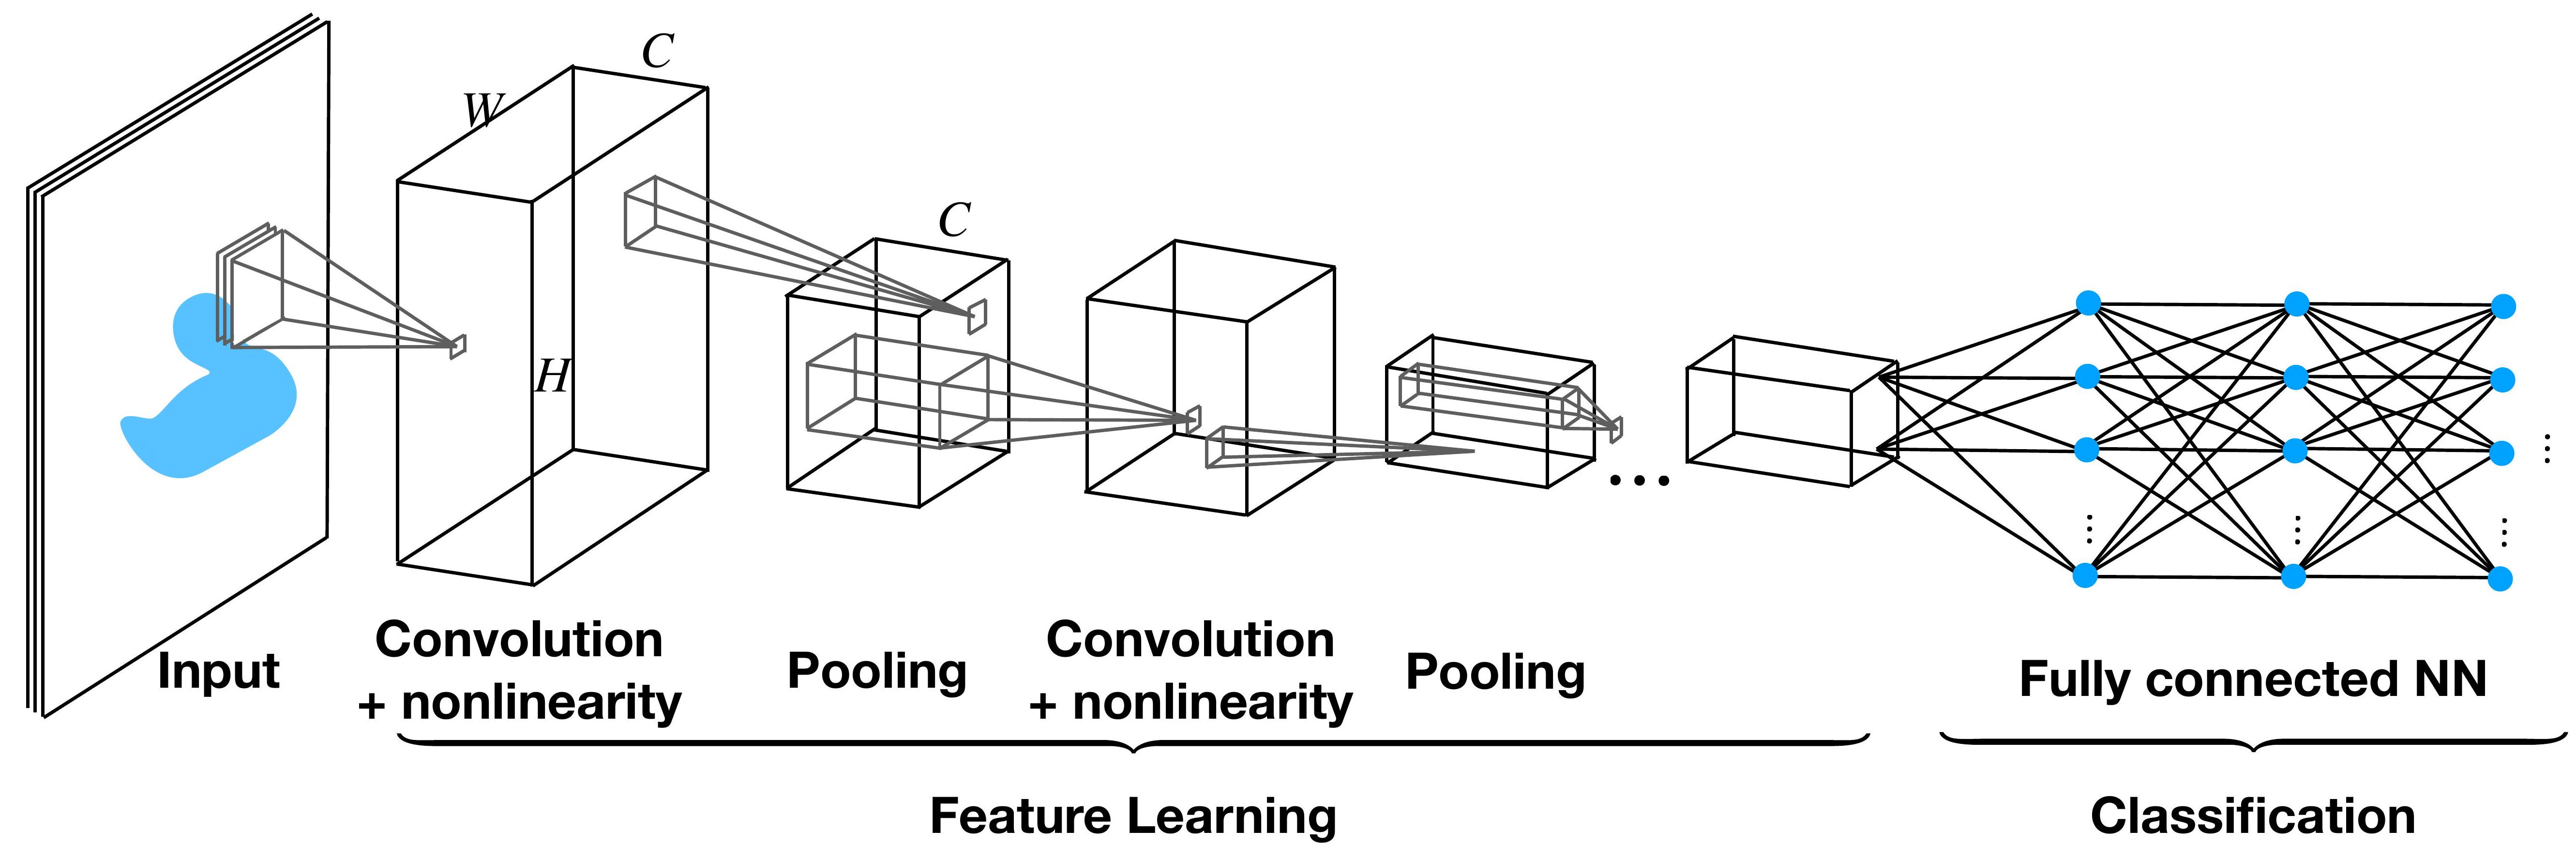
\includegraphics[max width=\textwidth]{2024_01_08_959e2db67a31f073f6d2g-03}
\end{center}

\begin{itemize}
  \item Convolutional networks consist of sparsely connected convolutional layers in place of fully-connected linear layers
  \item Pooling layers perform spatial downsampling (typically typically reducing the dimensions from $H \times W$ to $H / 2 \times W / 2$
  \item A fully-connected network at the end performs classification based on the extracted features
\end{itemize}

\section*{Fully connected NNs have many parameters and do not capture spatial dependencies }
\begin{itemize}
  \item Fully connected NNs have $O\left(K^{2} L\right)$ parameters: training requires a lot of data
\end{itemize}

\begin{center}
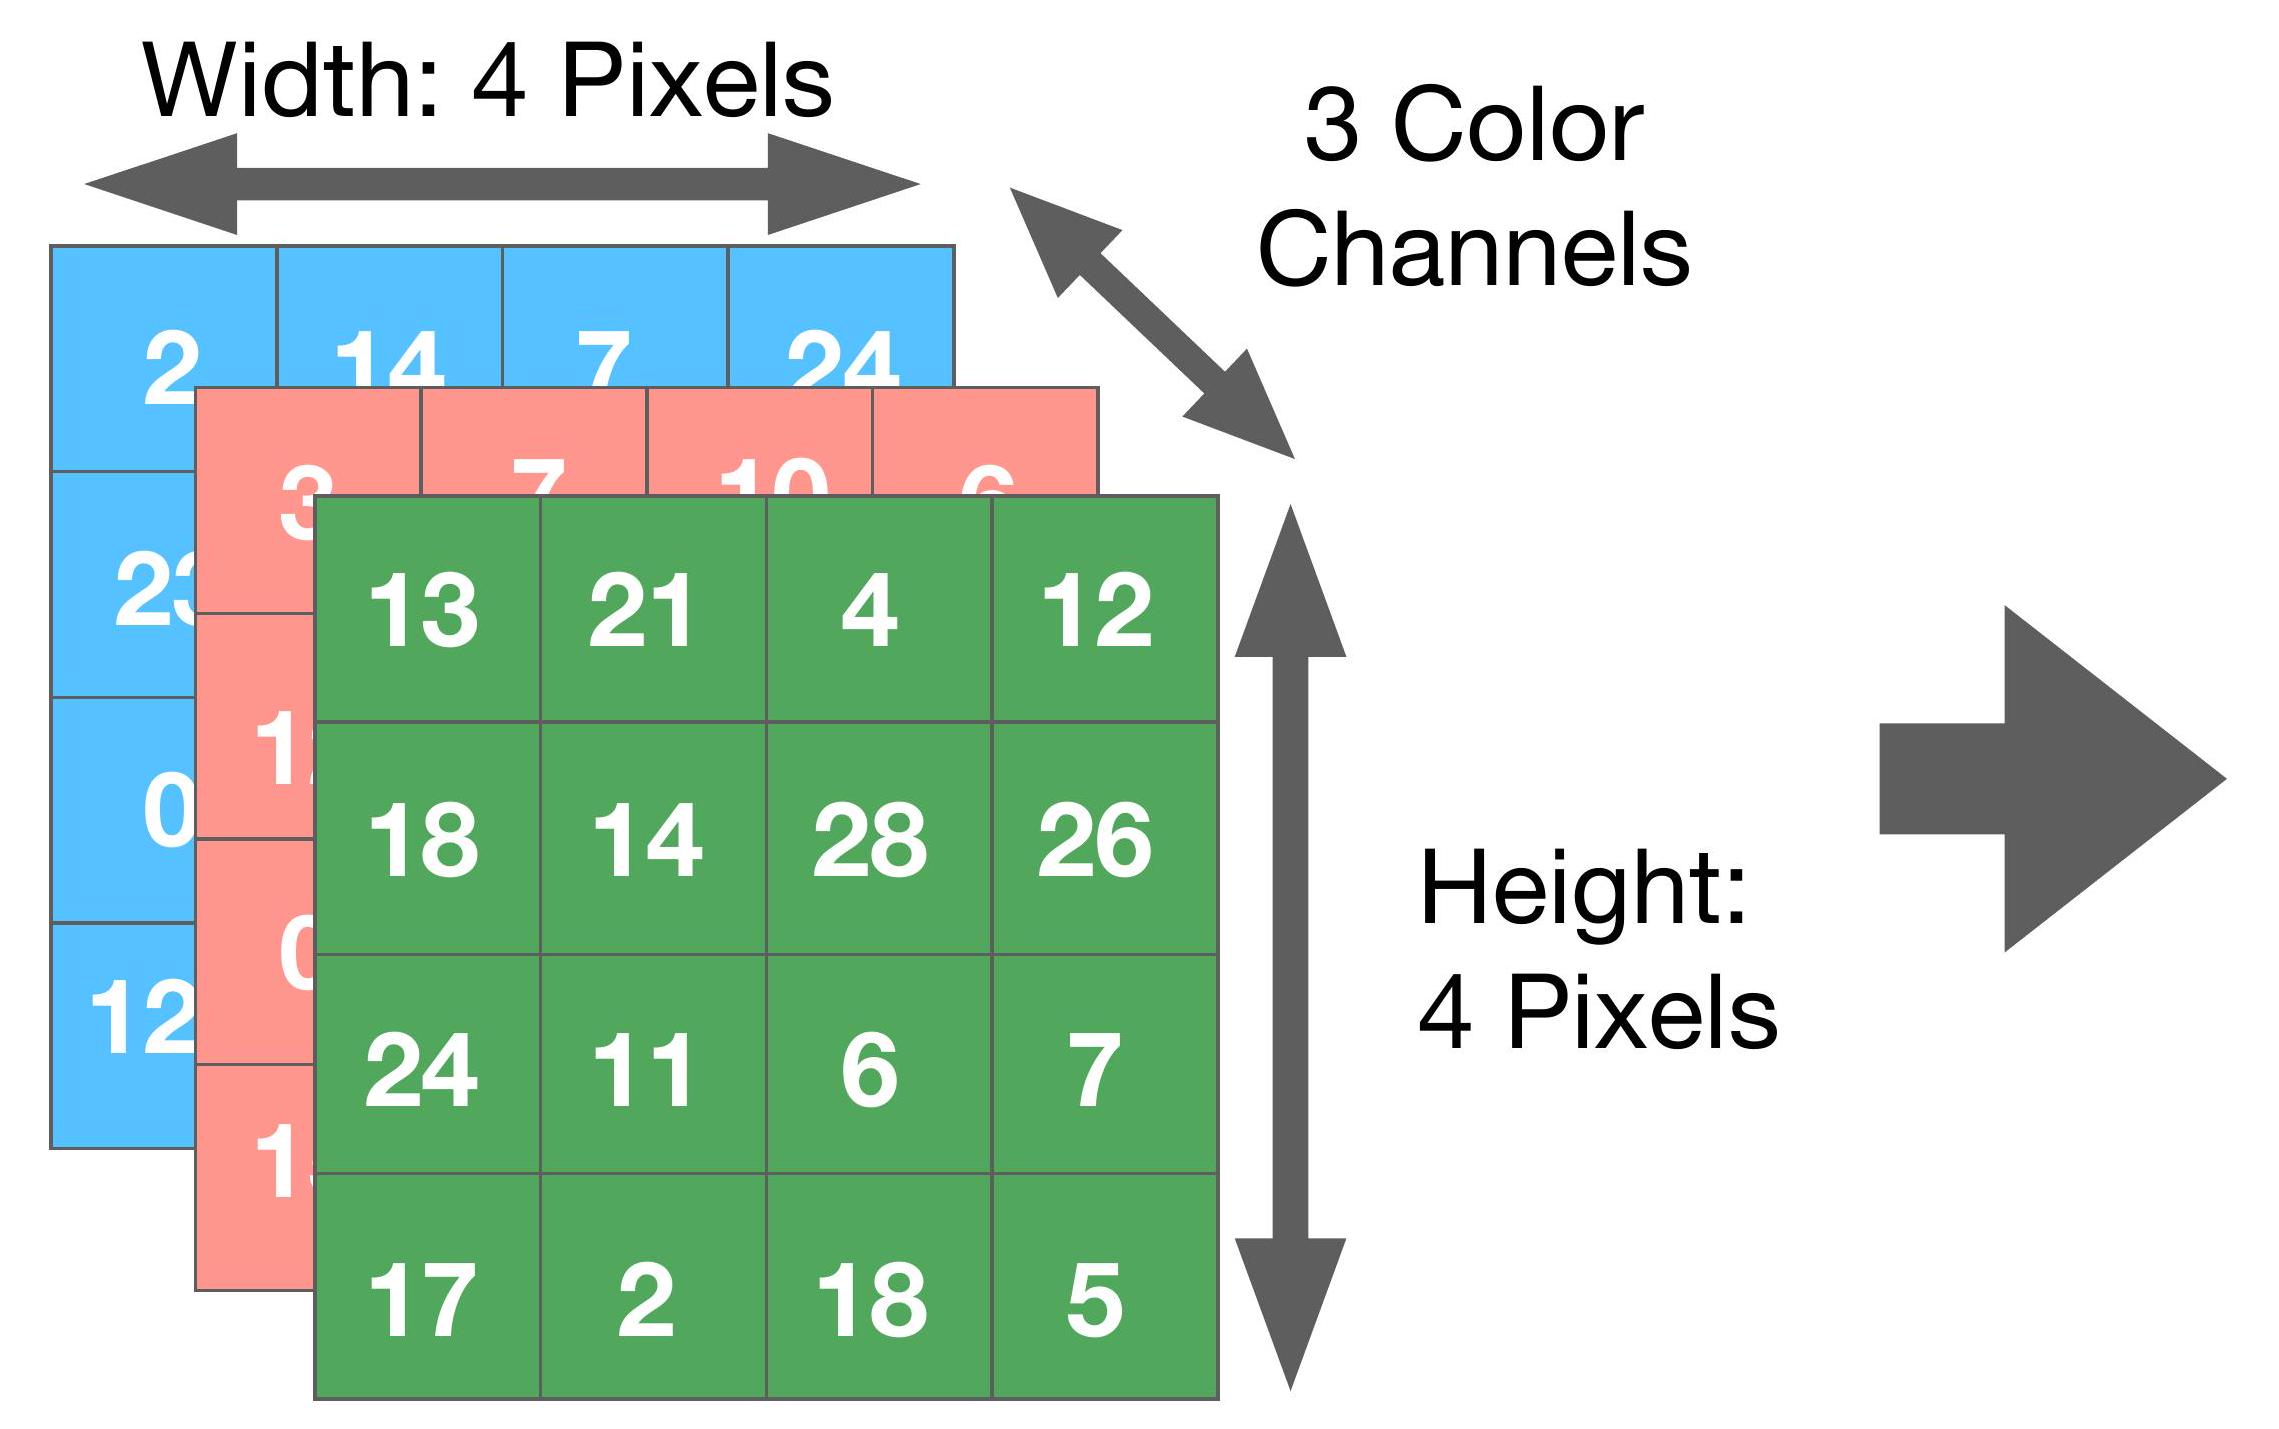
\includegraphics[max width=\textwidth]{2024_01_08_959e2db67a31f073f6d2g-04(1)}
\end{center}



\begin{itemize}
  \item Fully connected neural networks interpret an image as a flattened vector, disregarding the original spatial dependencies
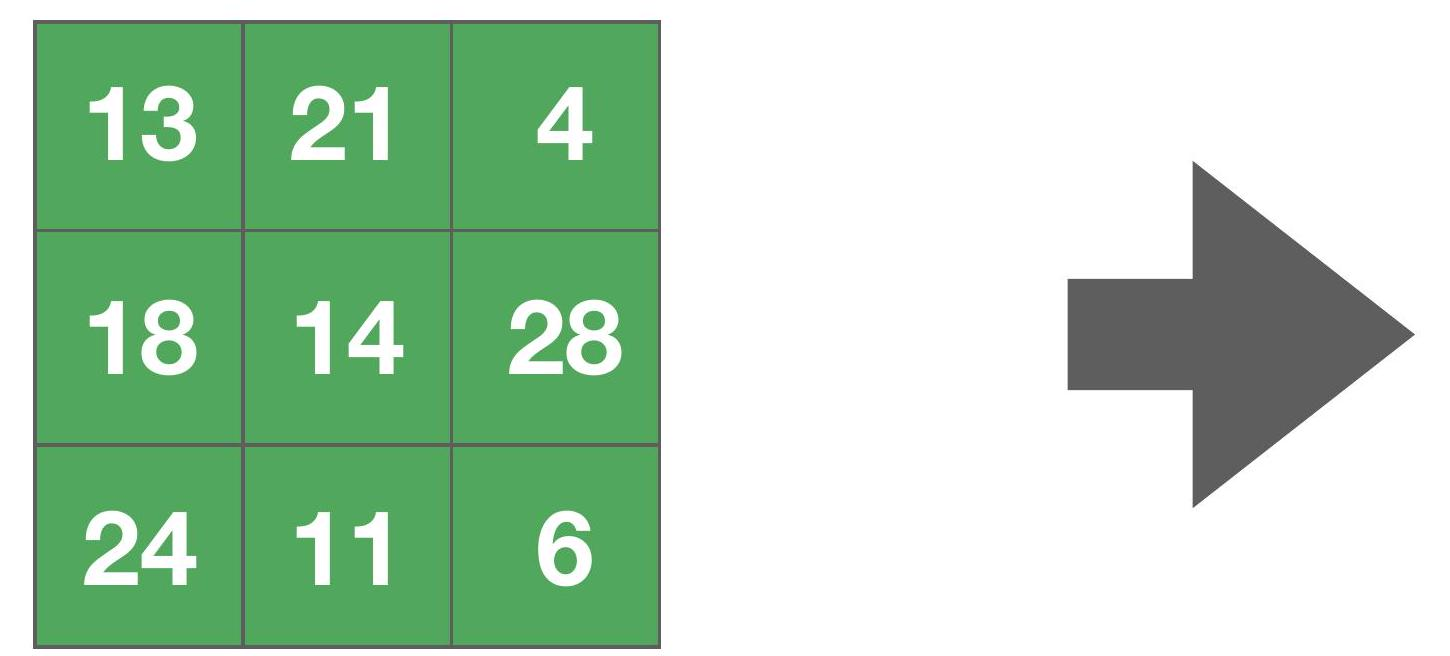
\includegraphics[max width=\textwidth, center]{2024_01_08_959e2db67a31f073f6d2g-04}
\end{itemize}

$$
\begin{array}{l|l|l|l|l|l|l|l|l}
13 & 21 & 4 & 18 & 14 & 28 & 24 & 11 & 6
\end{array}
$$

\section*{Convolution}
$$
x_{n, m}^{(1)}=\sum_{k, l} f_{k, l} \cdot x_{n-k, m-l}^{(0)}
$$

\begin{itemize}
  \item We consider local filters: $f_{k, l} \neq 0$ for small values of $|k|$ and $|l|$
\end{itemize}

$\Rightarrow x_{n, m}^{(1)}$ only depends on the value of $x^{(0)}$ close to $(n, m)$

$\Rightarrow f$ represents the learnable weights

\begin{itemize}
  \item We use the same filter at every position - weight sharing

  \item Translation equivariance - a shifted input results in a shifted output

\end{itemize}

\begin{center}
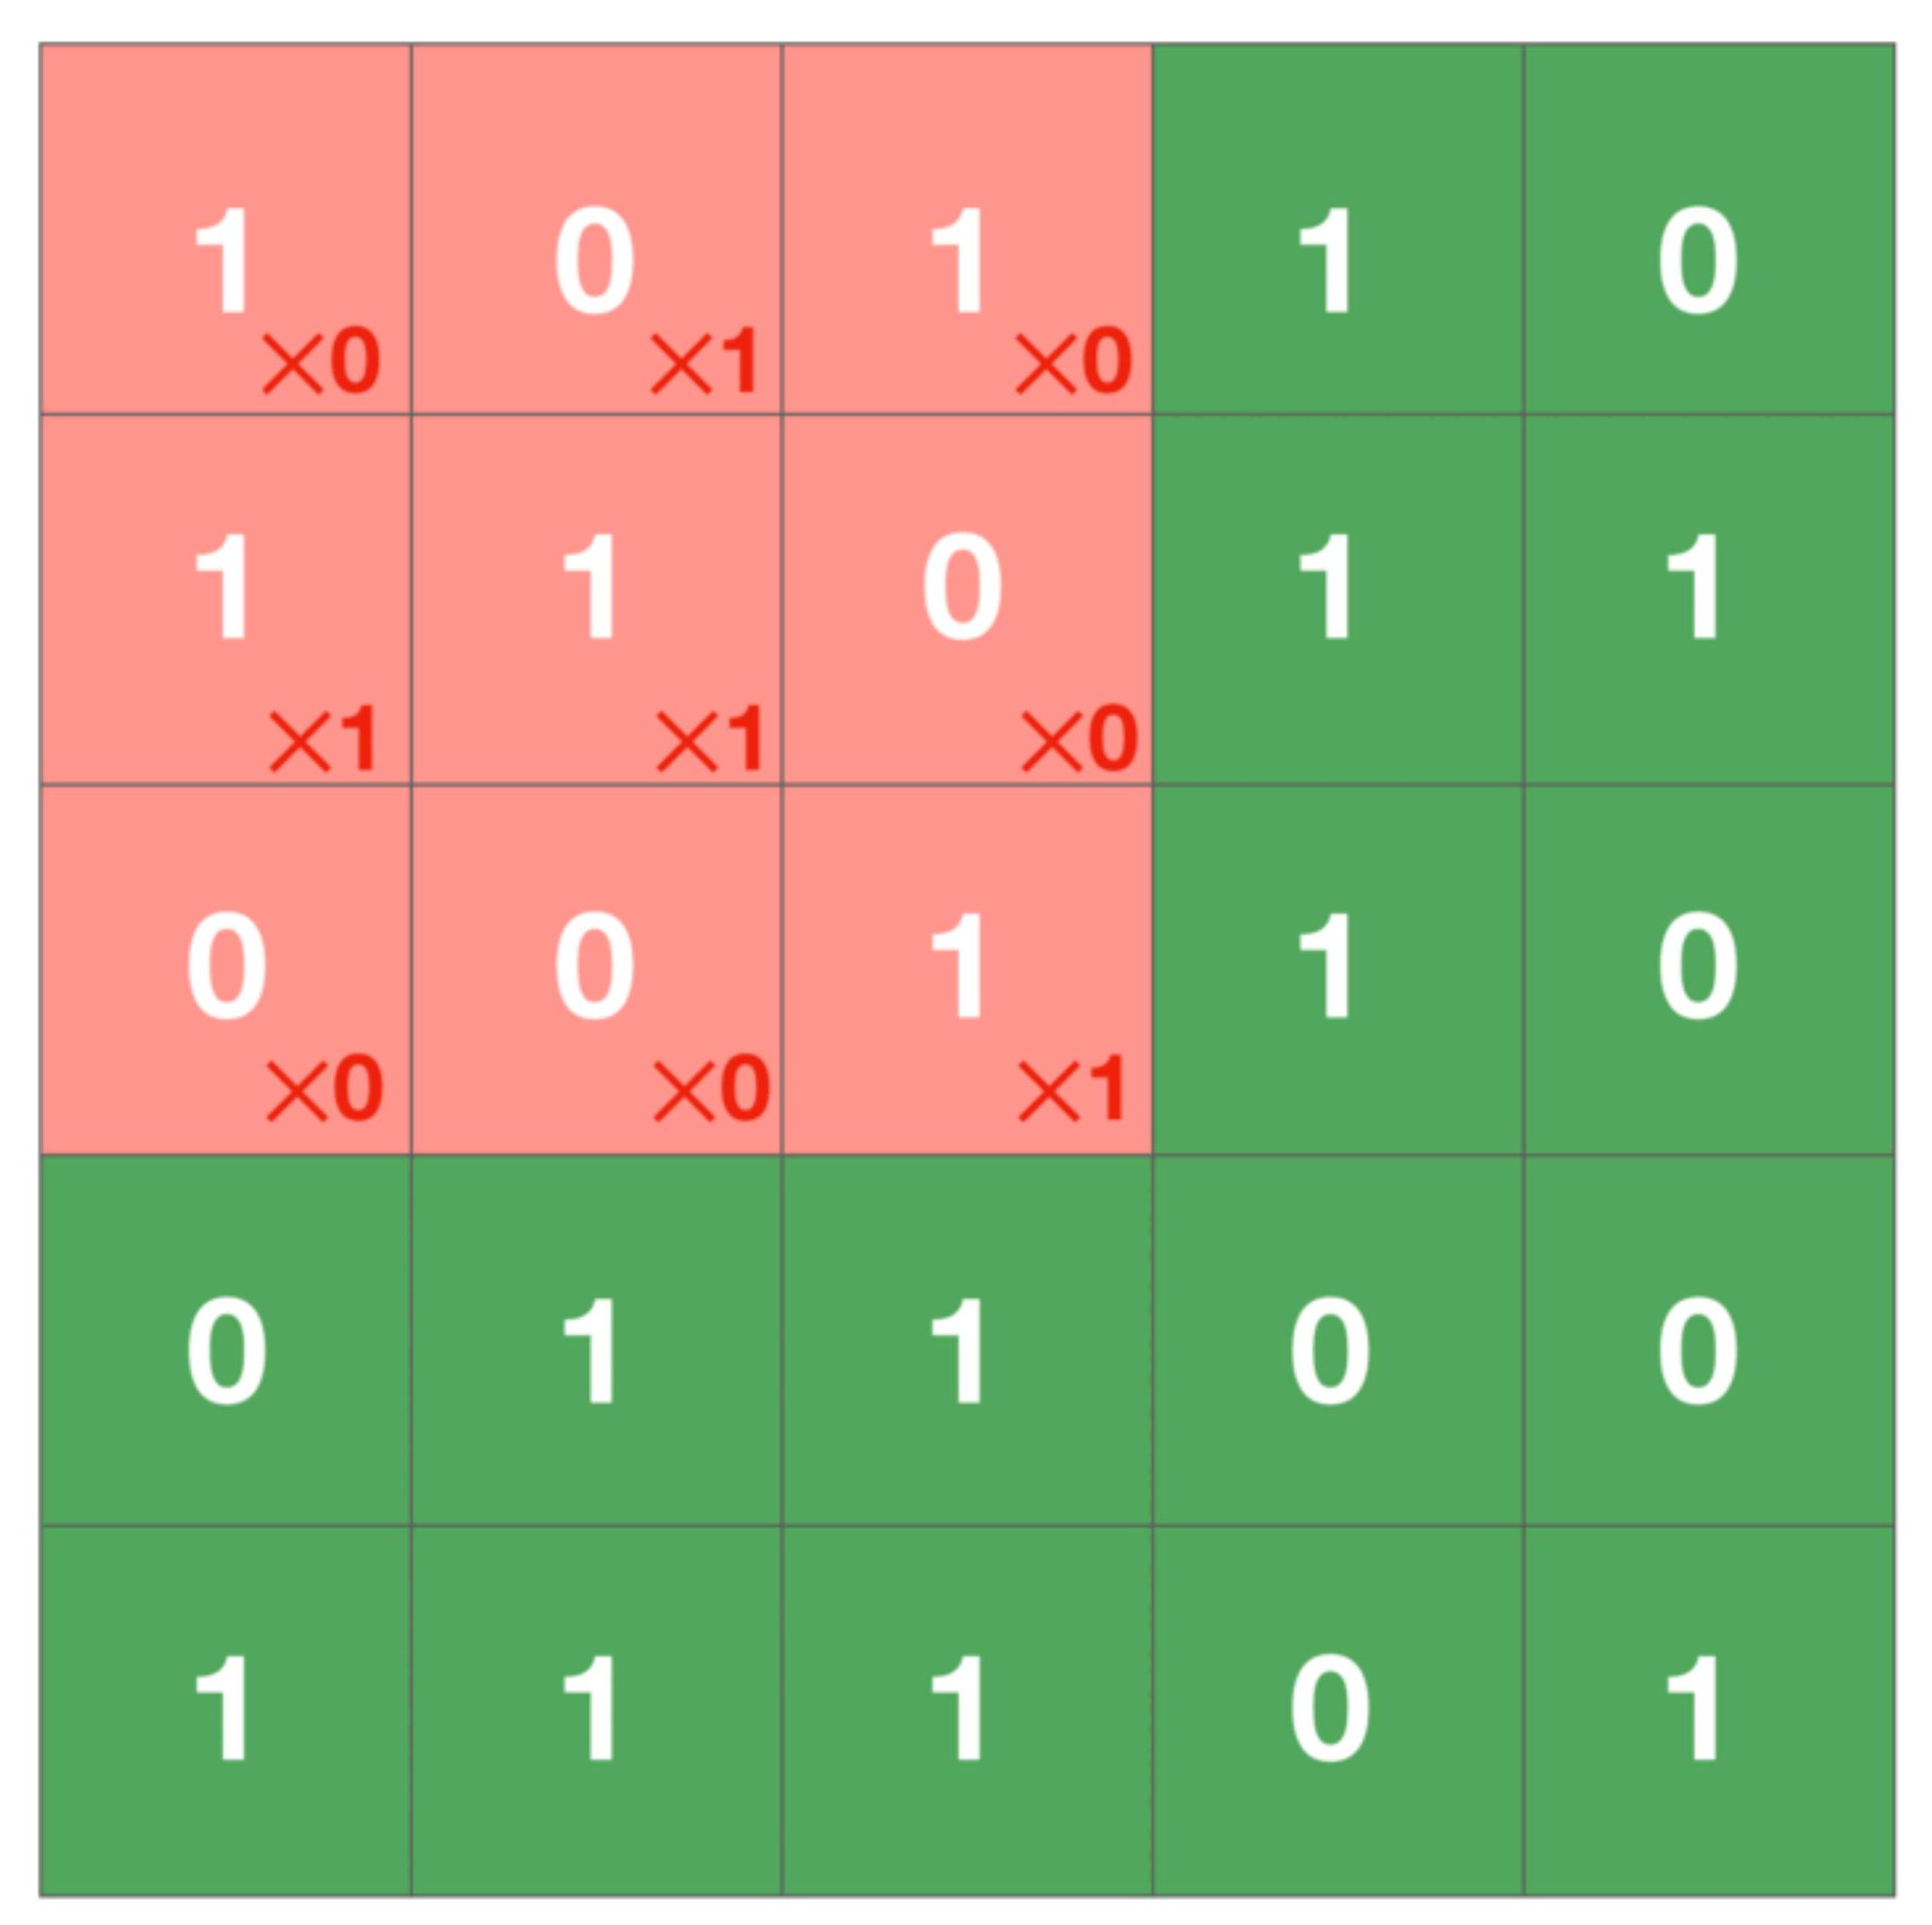
\includegraphics[max width=\textwidth]{2024_01_08_959e2db67a31f073f6d2g-05}
\end{center}

Image

$\Rightarrow$ Convolution requires fewer parameters which are universal across different locations

\section*{Handling of borders}
Zero padding:
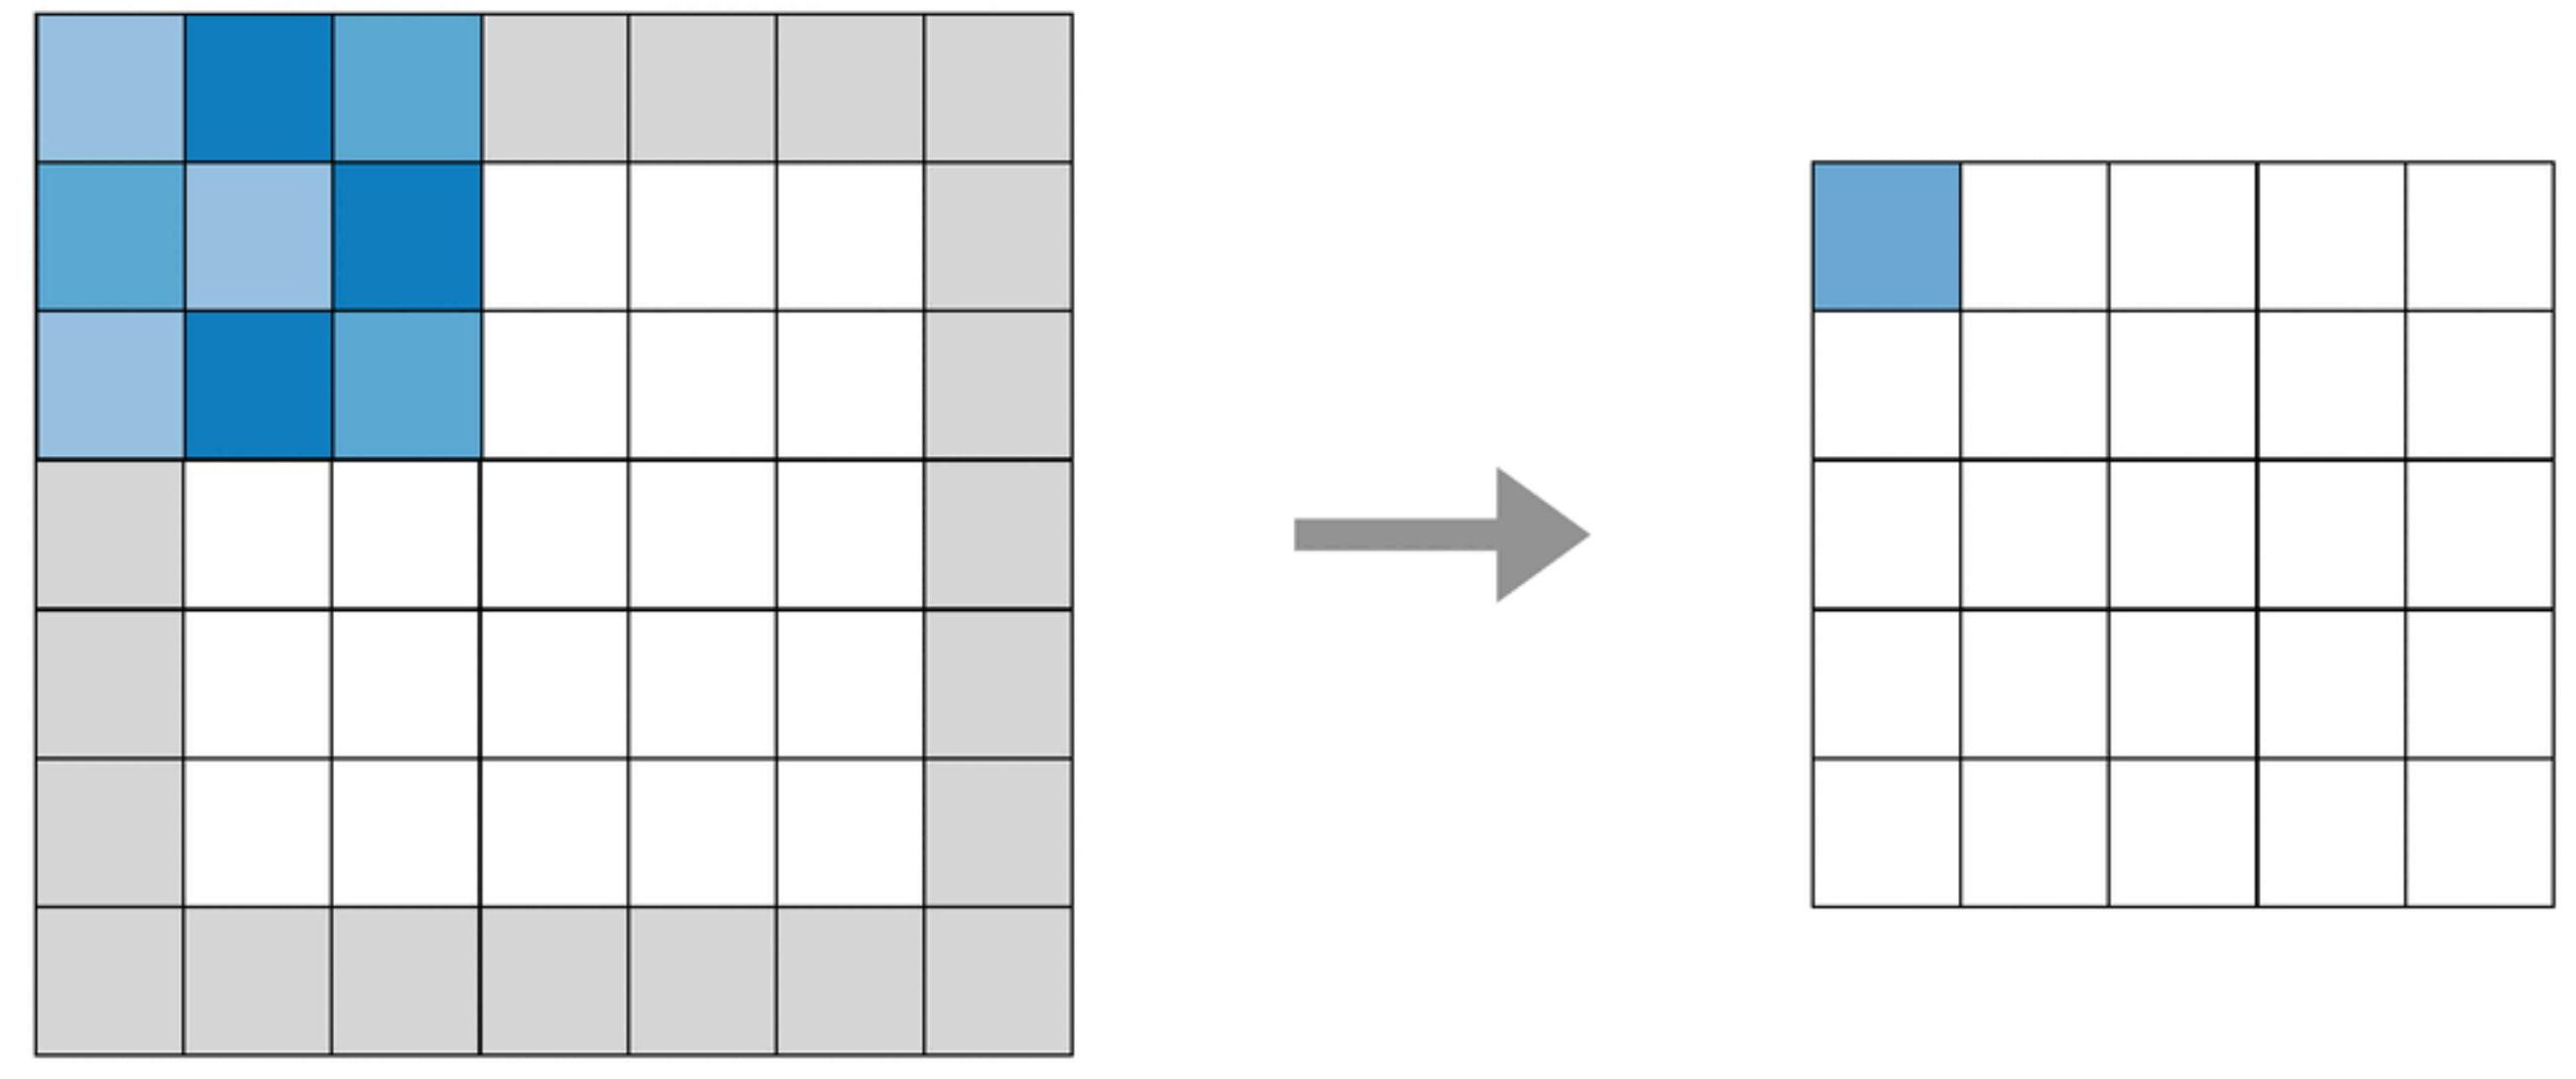
\includegraphics[max width=\textwidth, center]{2024_01_08_959e2db67a31f073f6d2g-06(1)}

Add zeros to each side of the input's boundaries

$\Rightarrow$ The convolved feature has the same dimension as the input
Valid padding:

\begin{center}
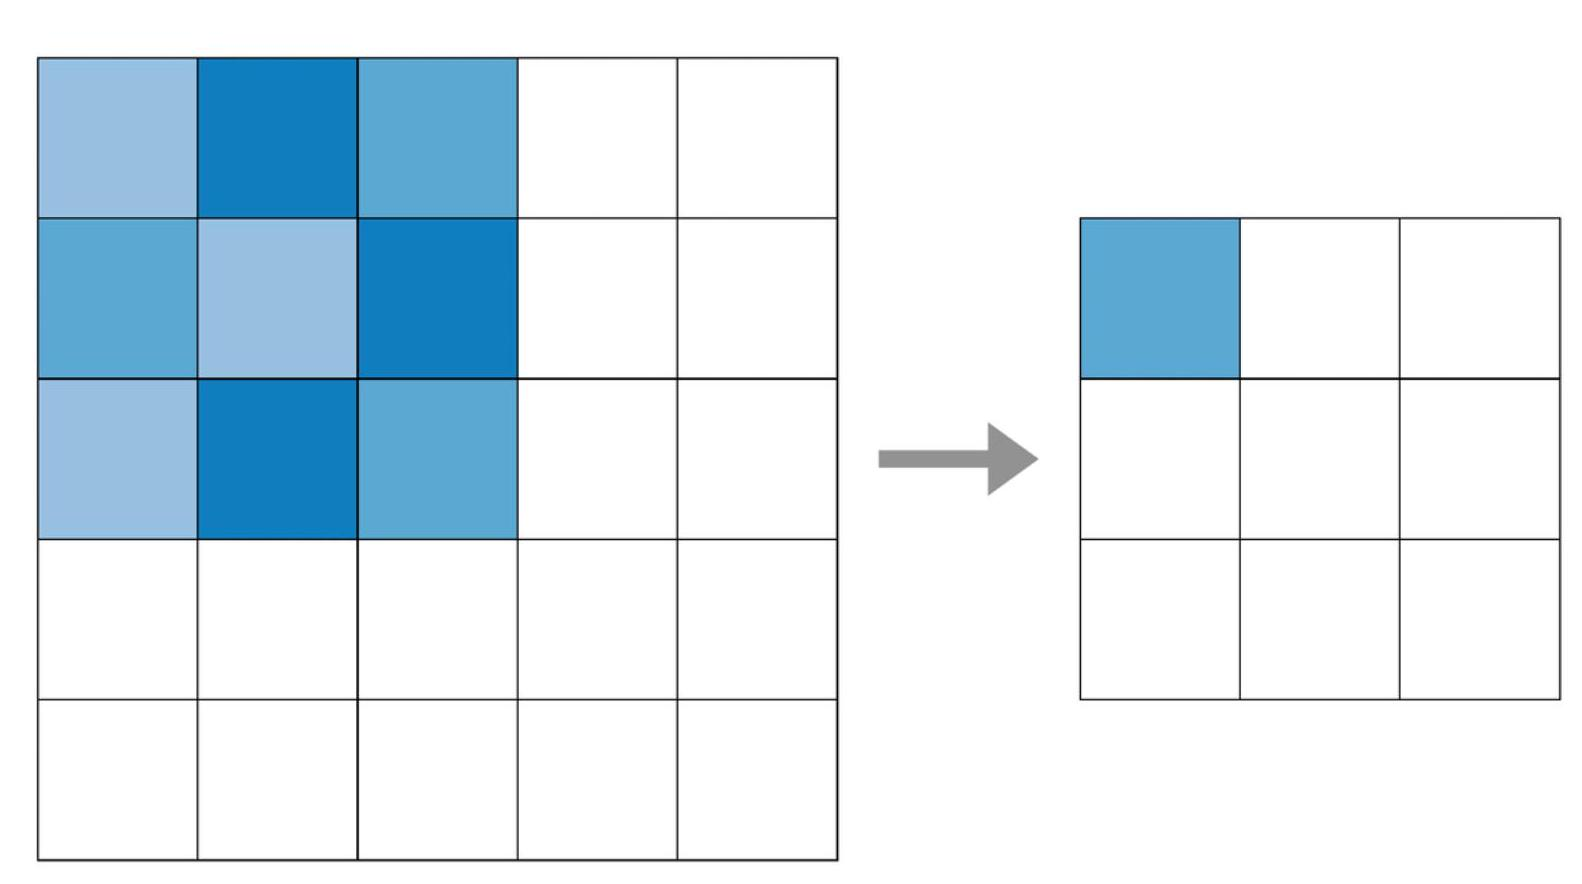
\includegraphics[max width=\textwidth]{2024_01_08_959e2db67a31f073f6d2g-06}
\end{center}

Perform the convolution only where the entire filter fits inside the original data

$\Rightarrow$ The convolved feature has smaller dimensions than the input

\section*{Filter for Multi-Channel Convolution}
\begin{center}
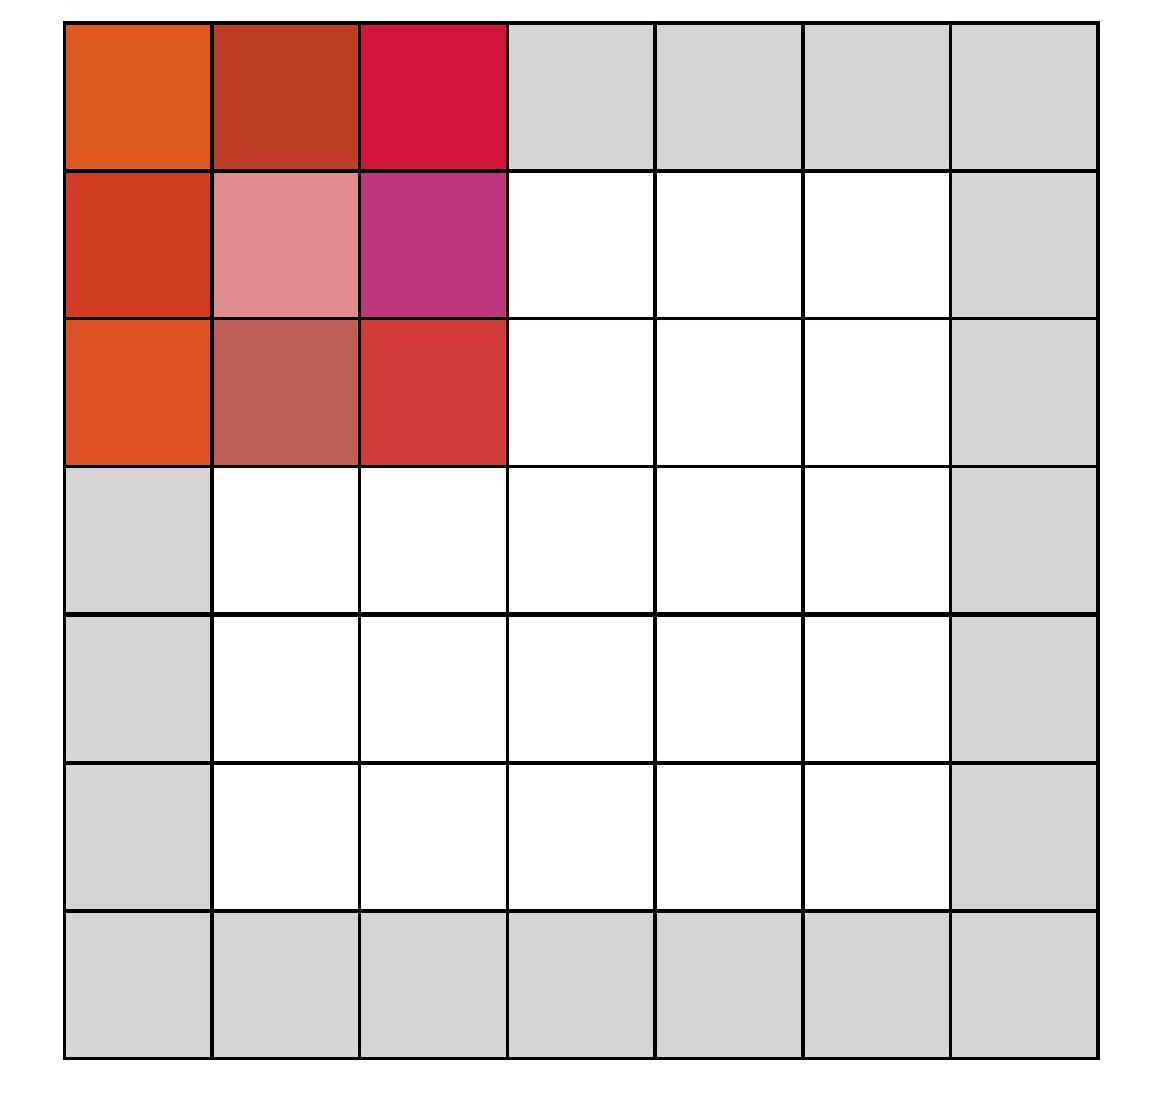
\includegraphics[max width=\textwidth]{2024_01_08_959e2db67a31f073f6d2g-07(1)}
\end{center}

Input Channel \#1

\begin{center}
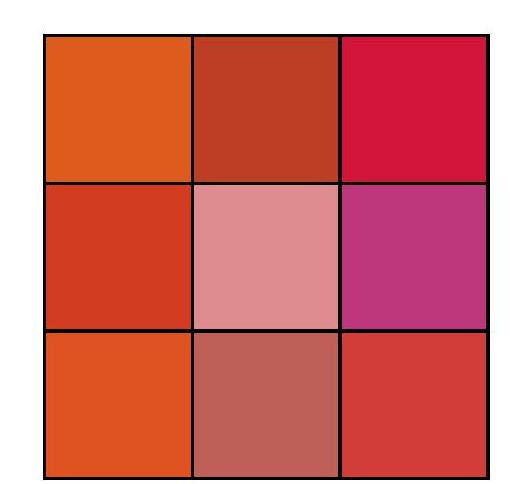
\includegraphics[max width=\textwidth]{2024_01_08_959e2db67a31f073f6d2g-07(5)}
\end{center}

Filter Channel \#1

\begin{center}
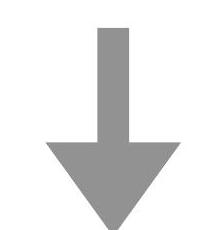
\includegraphics[max width=\textwidth]{2024_01_08_959e2db67a31f073f6d2g-07(3)}
\end{center}

120

\begin{center}
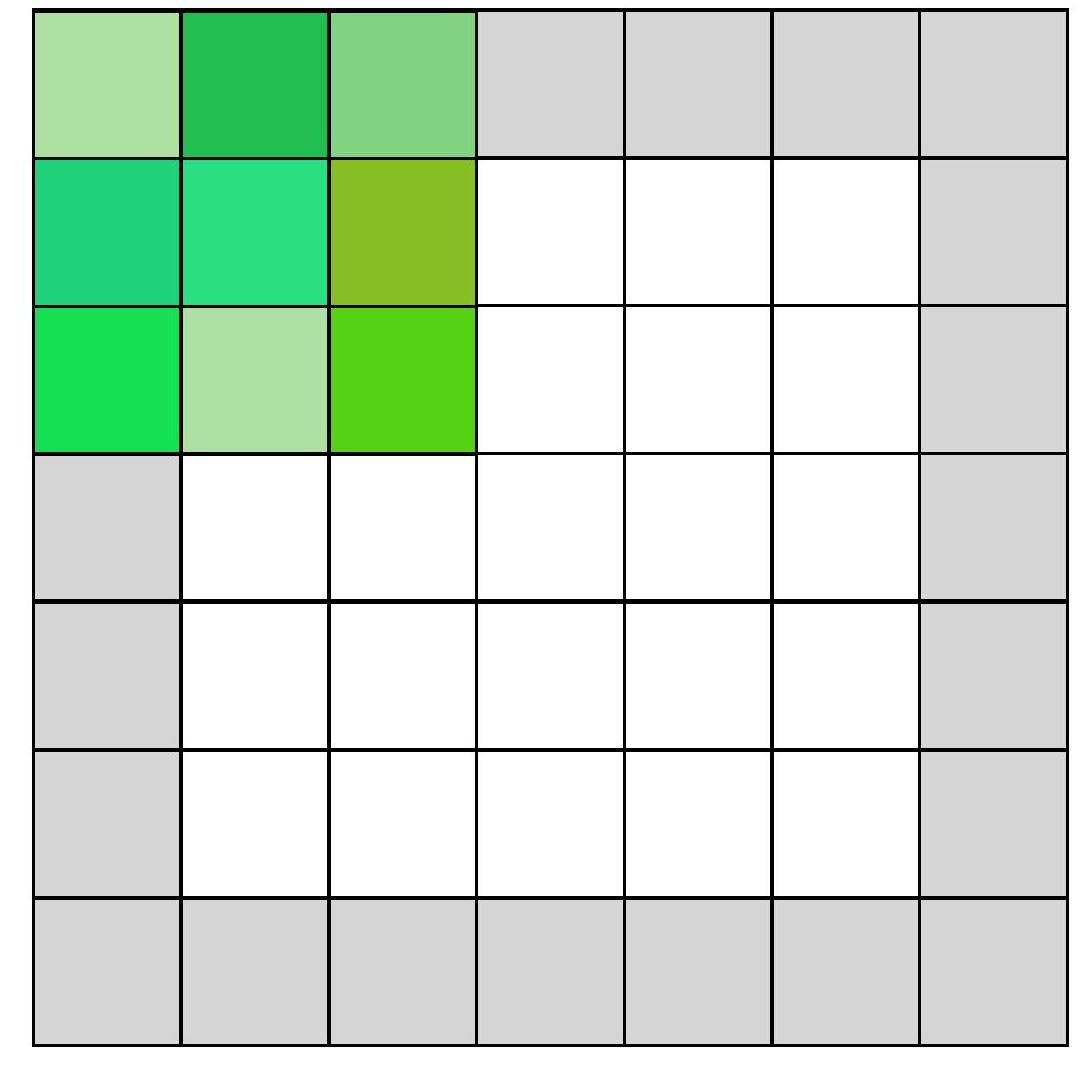
\includegraphics[max width=\textwidth]{2024_01_08_959e2db67a31f073f6d2g-07(7)}
\end{center}

Input Channel \#2

\begin{center}
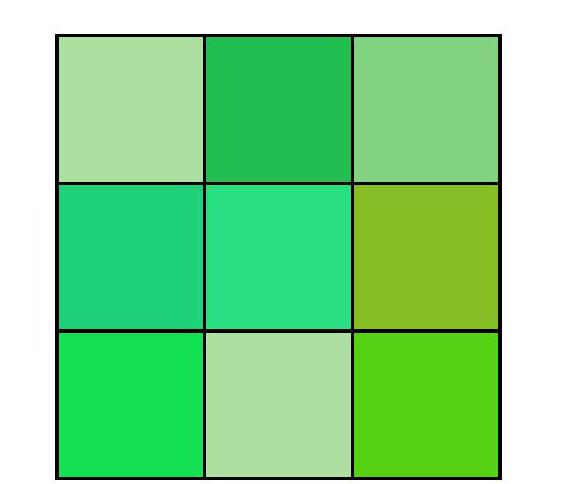
\includegraphics[max width=\textwidth]{2024_01_08_959e2db67a31f073f6d2g-07(8)}
\end{center}

Filter Channel \#2

\begin{center}
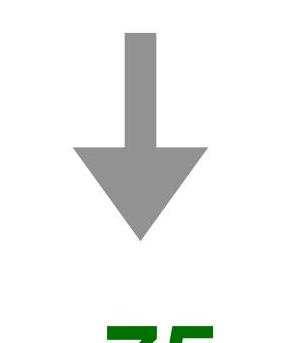
\includegraphics[max width=\textwidth]{2024_01_08_959e2db67a31f073f6d2g-07(4)}
\end{center}

\begin{center}
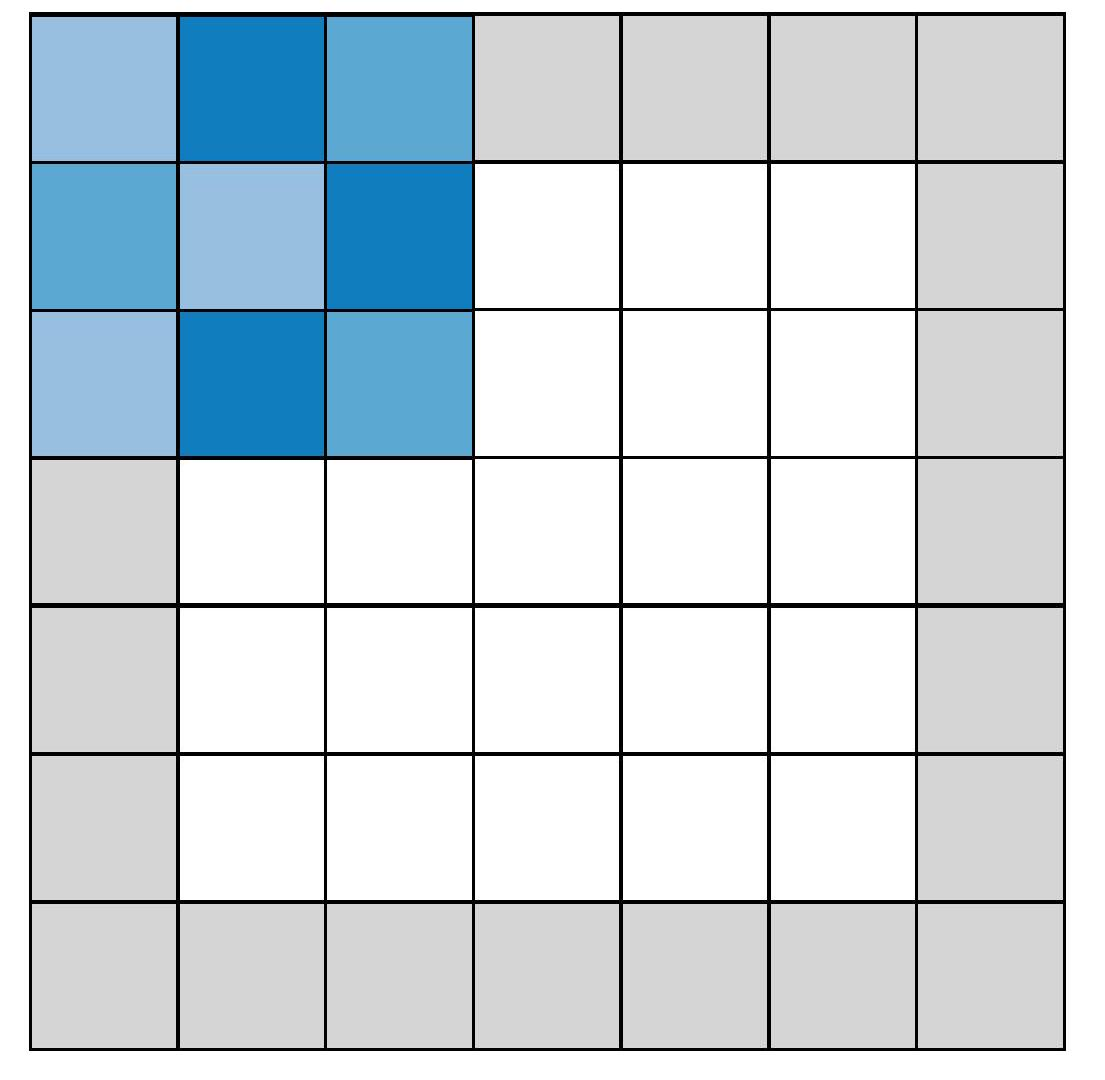
\includegraphics[max width=\textwidth]{2024_01_08_959e2db67a31f073f6d2g-07(6)}
\end{center}

Input Channel \#3

\begin{center}
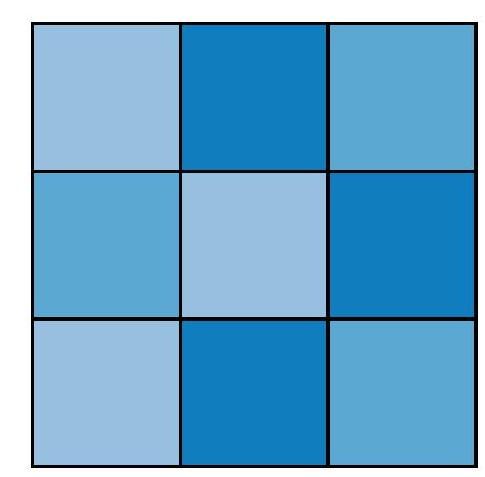
\includegraphics[max width=\textwidth]{2024_01_08_959e2db67a31f073f6d2g-07}
\end{center}

Filter Channel \#3

\begin{center}

\includegraphics[max width=\textwidth]{2024_01_08_959e2db67a31f073f6d2g-07(2)}
\end{center}

205

\begin{center}
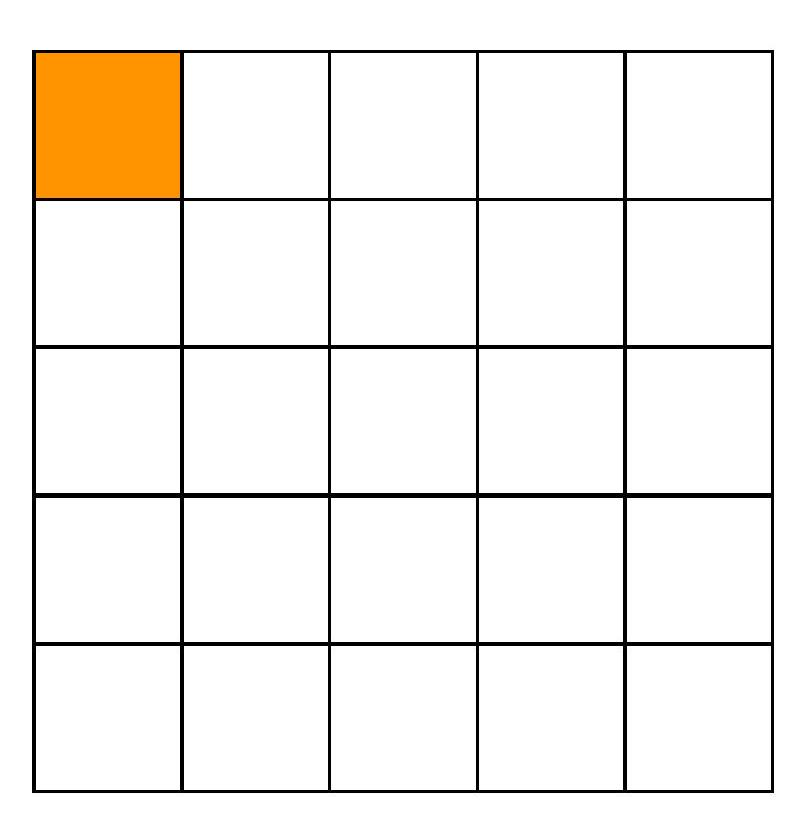
\includegraphics[max width=\textwidth]{2024_01_08_959e2db67a31f073f6d2g-07(9)}
\end{center}

One Channel Output

260

\begin{itemize}
  \item For multi-channel inputs, the filter has the same number of channels as the input
  \item The filter channels and the bias are the learnable parameters of the filter
\end{itemize}

\section*{Multi-Channel Output from Multiple Filters}
It is common to use multiple filters. Each filter processes the input to produce a separate channel

\begin{center}
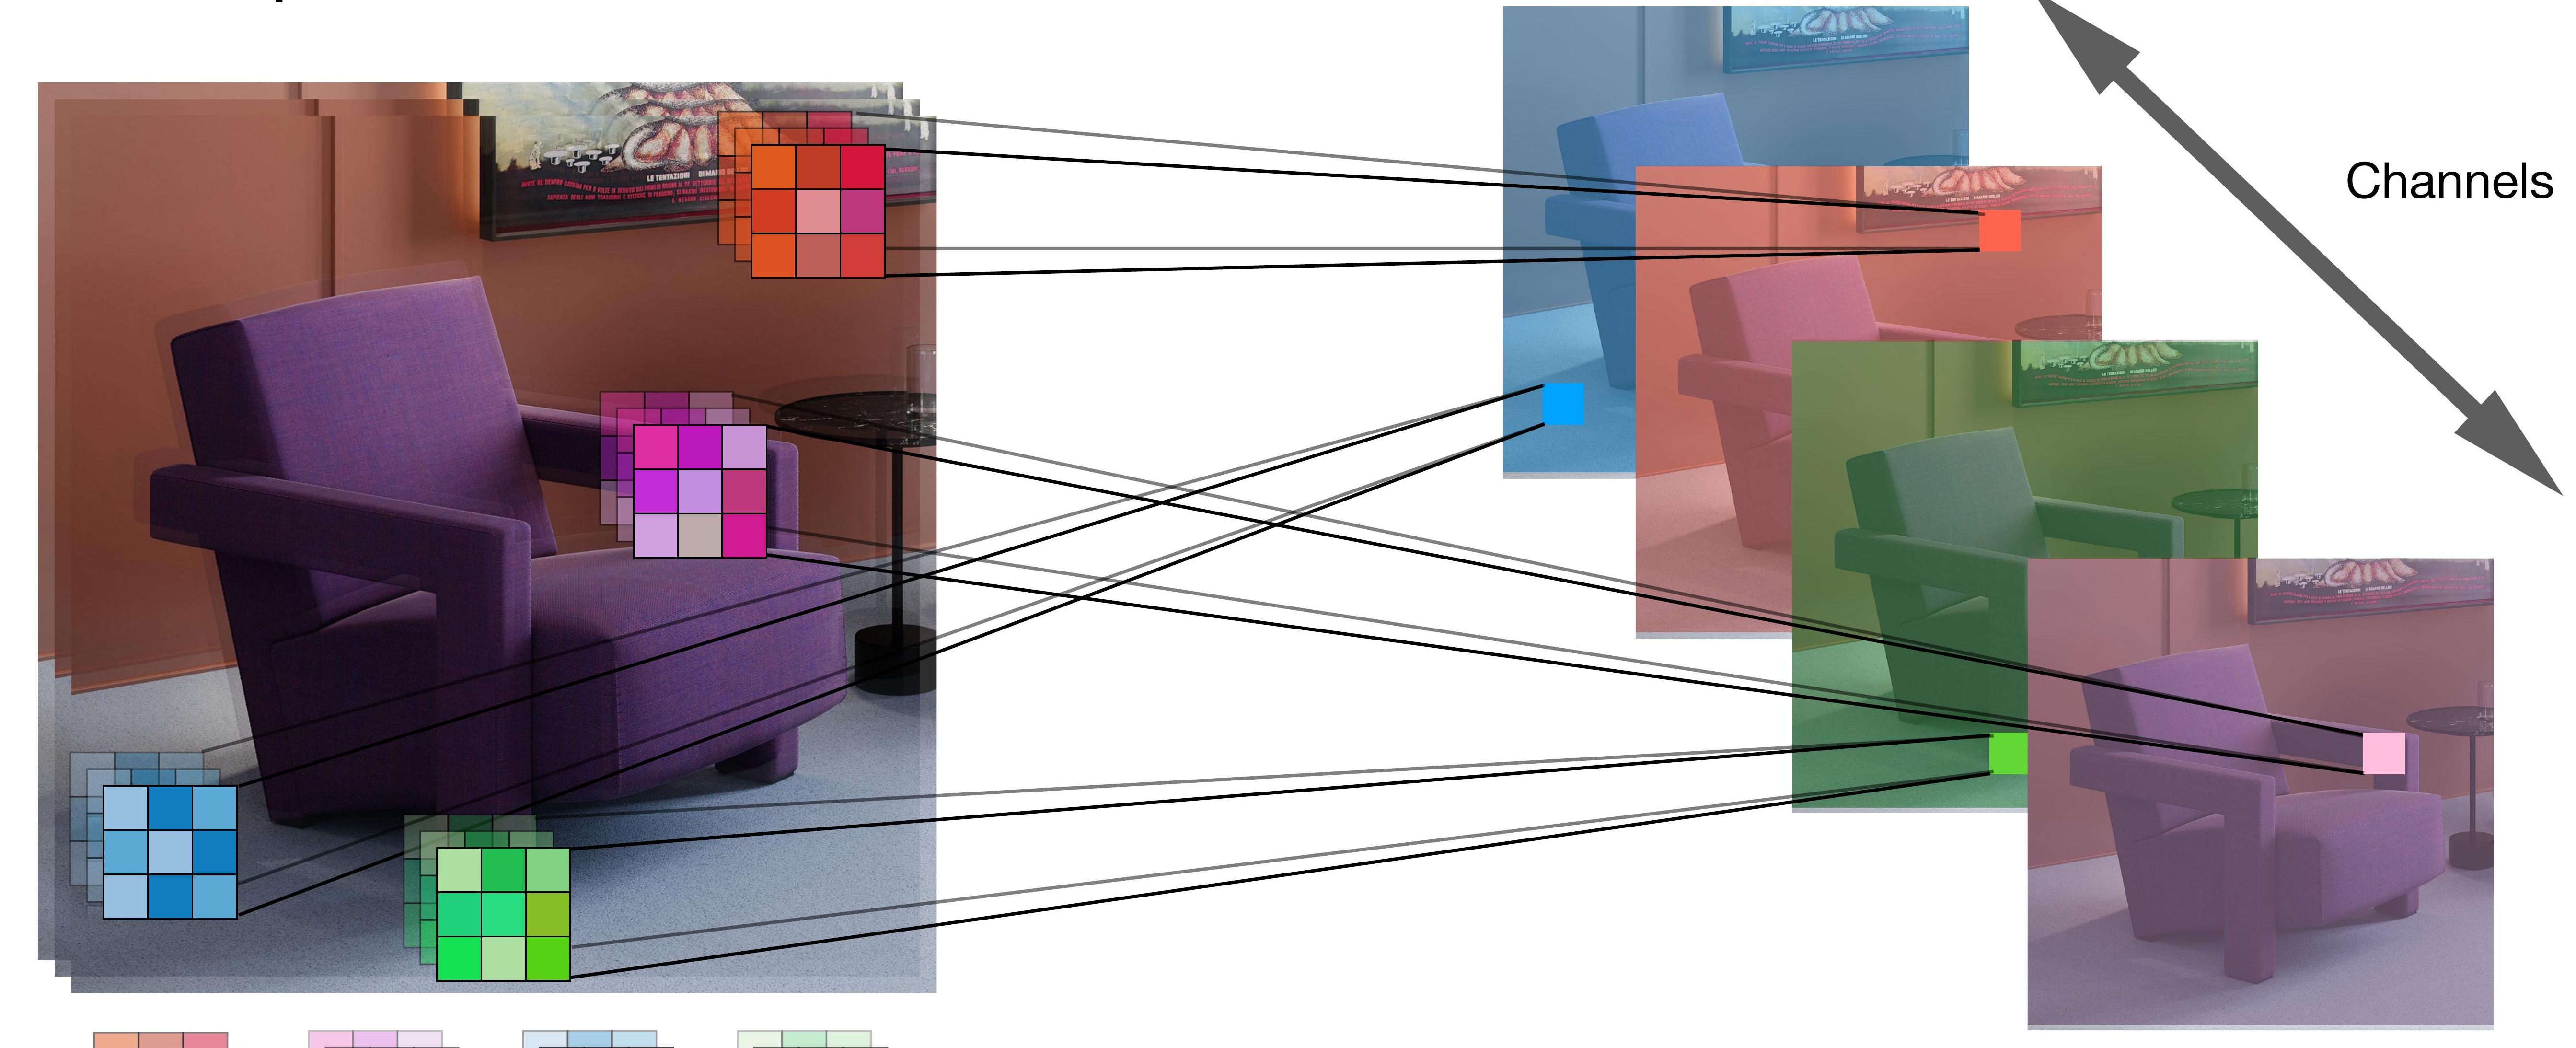
\includegraphics[max width=\textwidth]{2024_01_08_959e2db67a31f073f6d2g-08(1)}
\end{center}

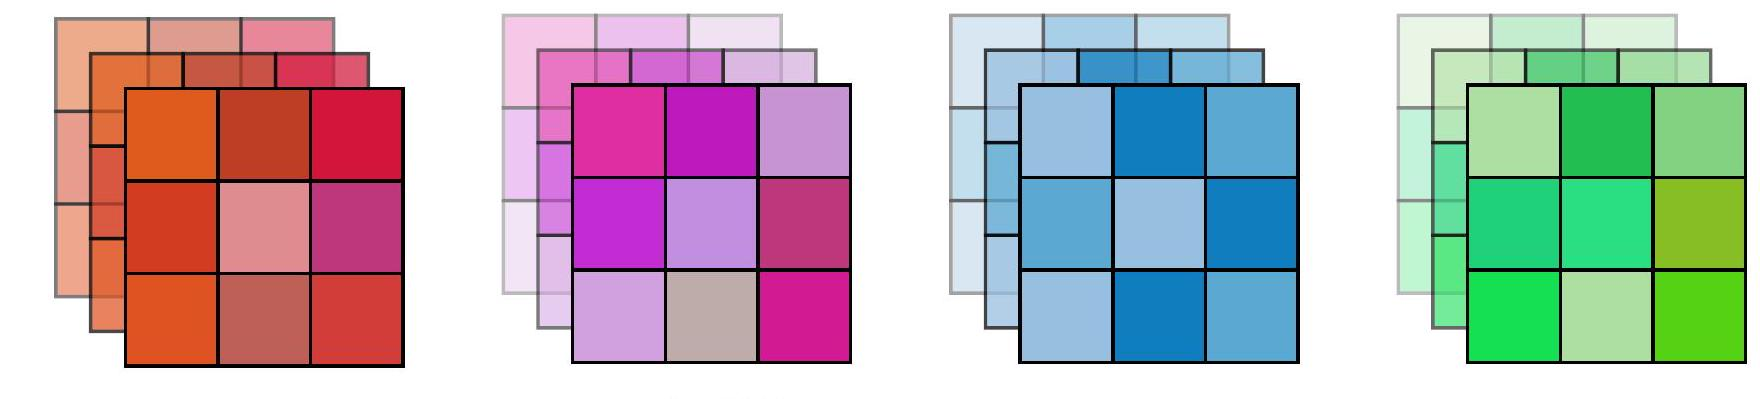
\includegraphics[max width=\textwidth, center]{2024_01_08_959e2db67a31f073f6d2g-08}
Filters
Applying different filters to an input generates multiple output channels.

\section*{Convolutional Layer}
\begin{center}
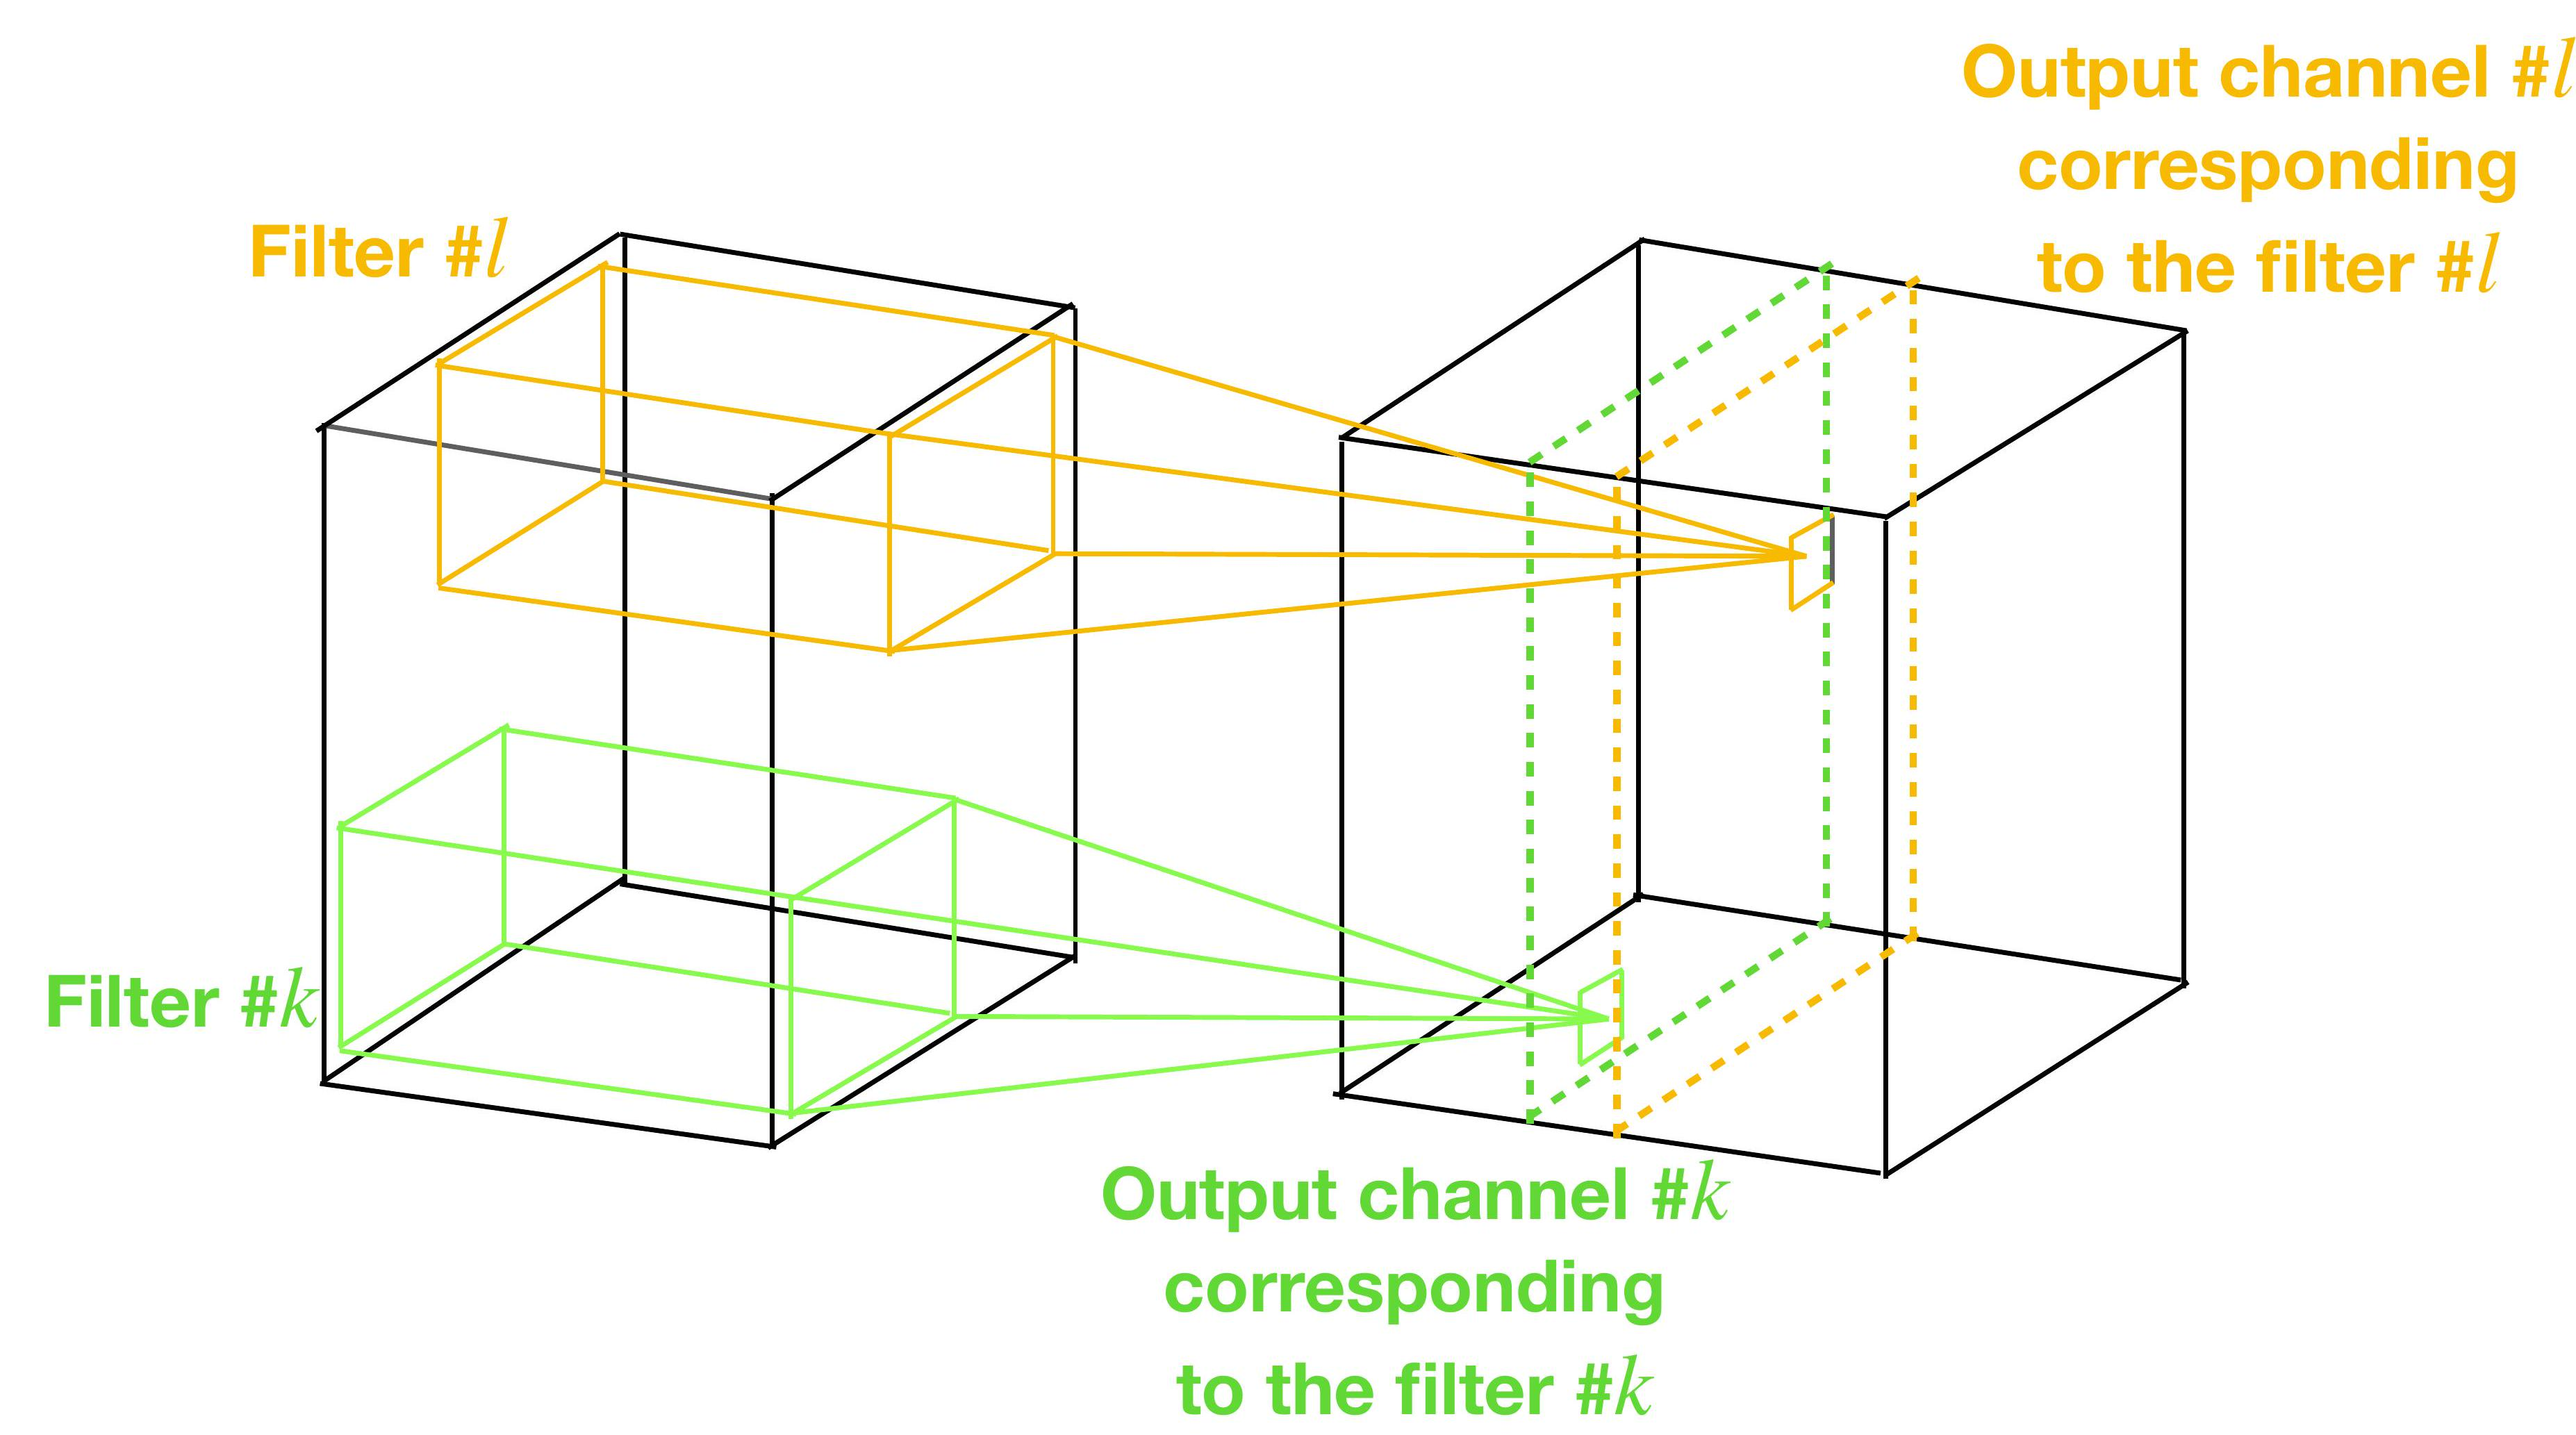
\includegraphics[max width=\textwidth]{2024_01_08_959e2db67a31f073f6d2g-09}
\end{center}

\begin{itemize}
  \item A convolutional layer is composed of multiple filters

  \item Each output channel corresponds to its own independent filter

  \item Hyper-parameters of the convolutional layer: size, padding, stride

\end{itemize}

\section*{Pooling: often applied after the convolutional layer}
Max pooling: returns the maximum value of the portion of the convolved feature that is covered by the kernel
Average pooling: returns the average value of the portion of the convolved feature that is covered by the kernel

\begin{center}
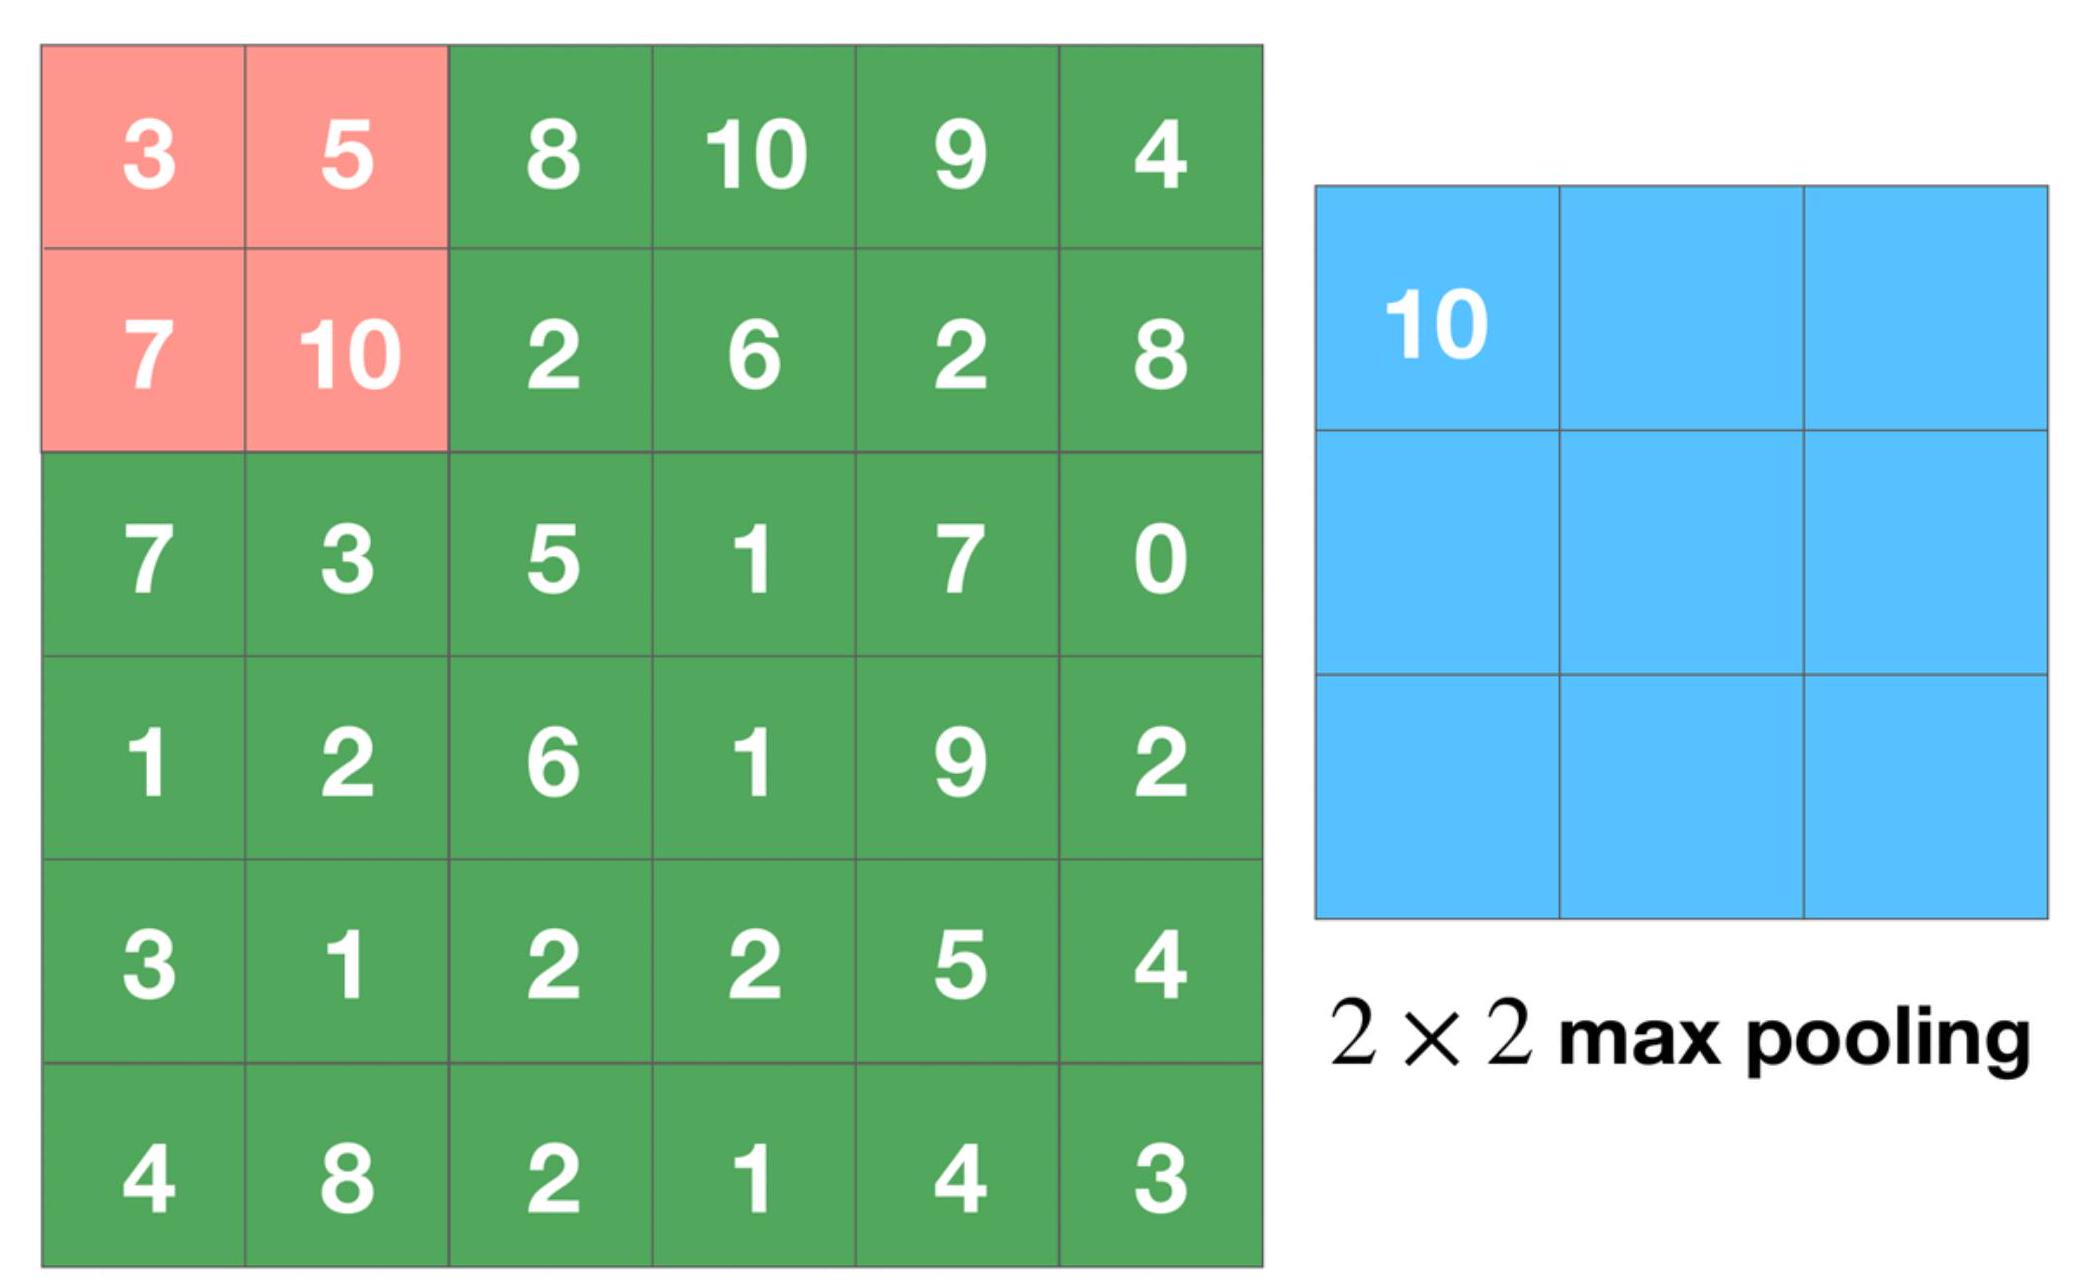
\includegraphics[max width=\textwidth]{2024_01_08_959e2db67a31f073f6d2g-10(1)}
\end{center}

Convolved feature

\begin{center}
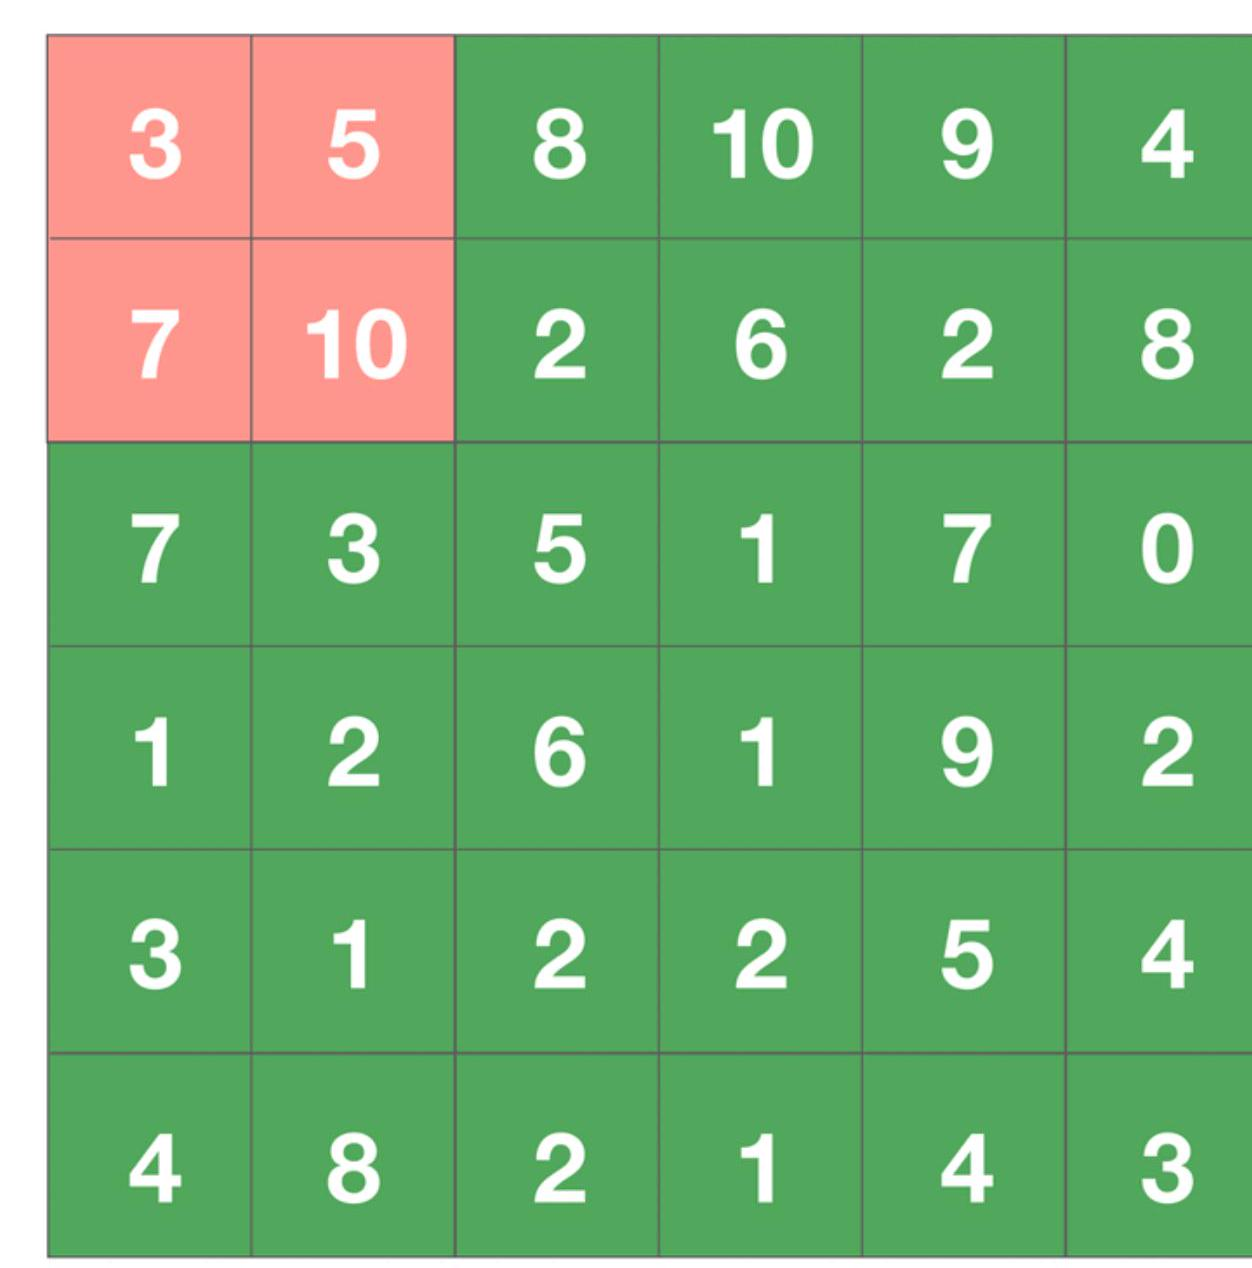
\includegraphics[max width=\textwidth]{2024_01_08_959e2db67a31f073f6d2g-10}
\end{center}

6.25

$2 \times 2$ average pooling

Convolved feature

Pooling is a downsampling operation that reduces the spatial dimensions of the convolved feature

Remark: Pooling layers do not have learnable parameters Hyperparameters are the size, type, and stride of the pooling operation

\section*{Non-linearity and convolutional NNs}
\begin{center}
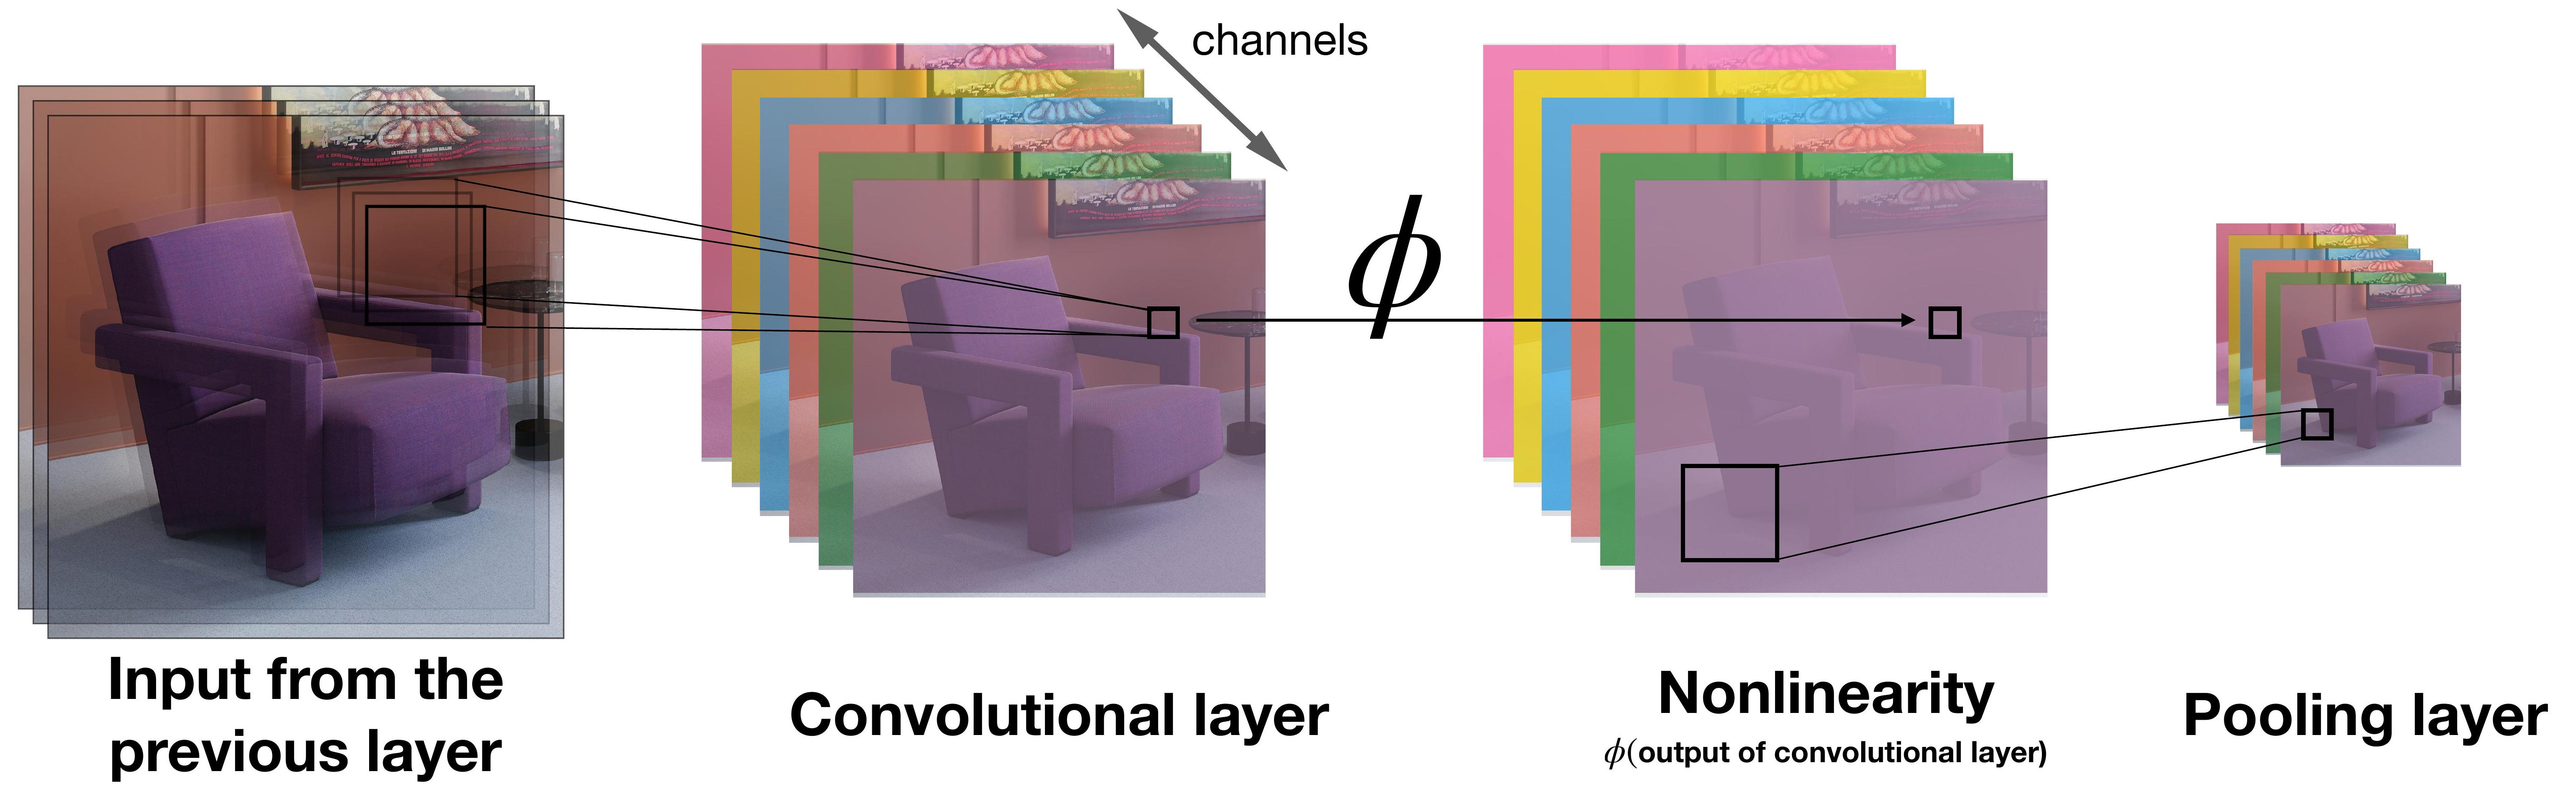
\includegraphics[max width=\textwidth]{2024_01_08_959e2db67a31f073f6d2g-11}
\end{center}

Important: A non-linearity such as ReLU is included after each convolutional layer to make the model non-linear

\section*{Convolutional NNs: General Structure}
\begin{center}
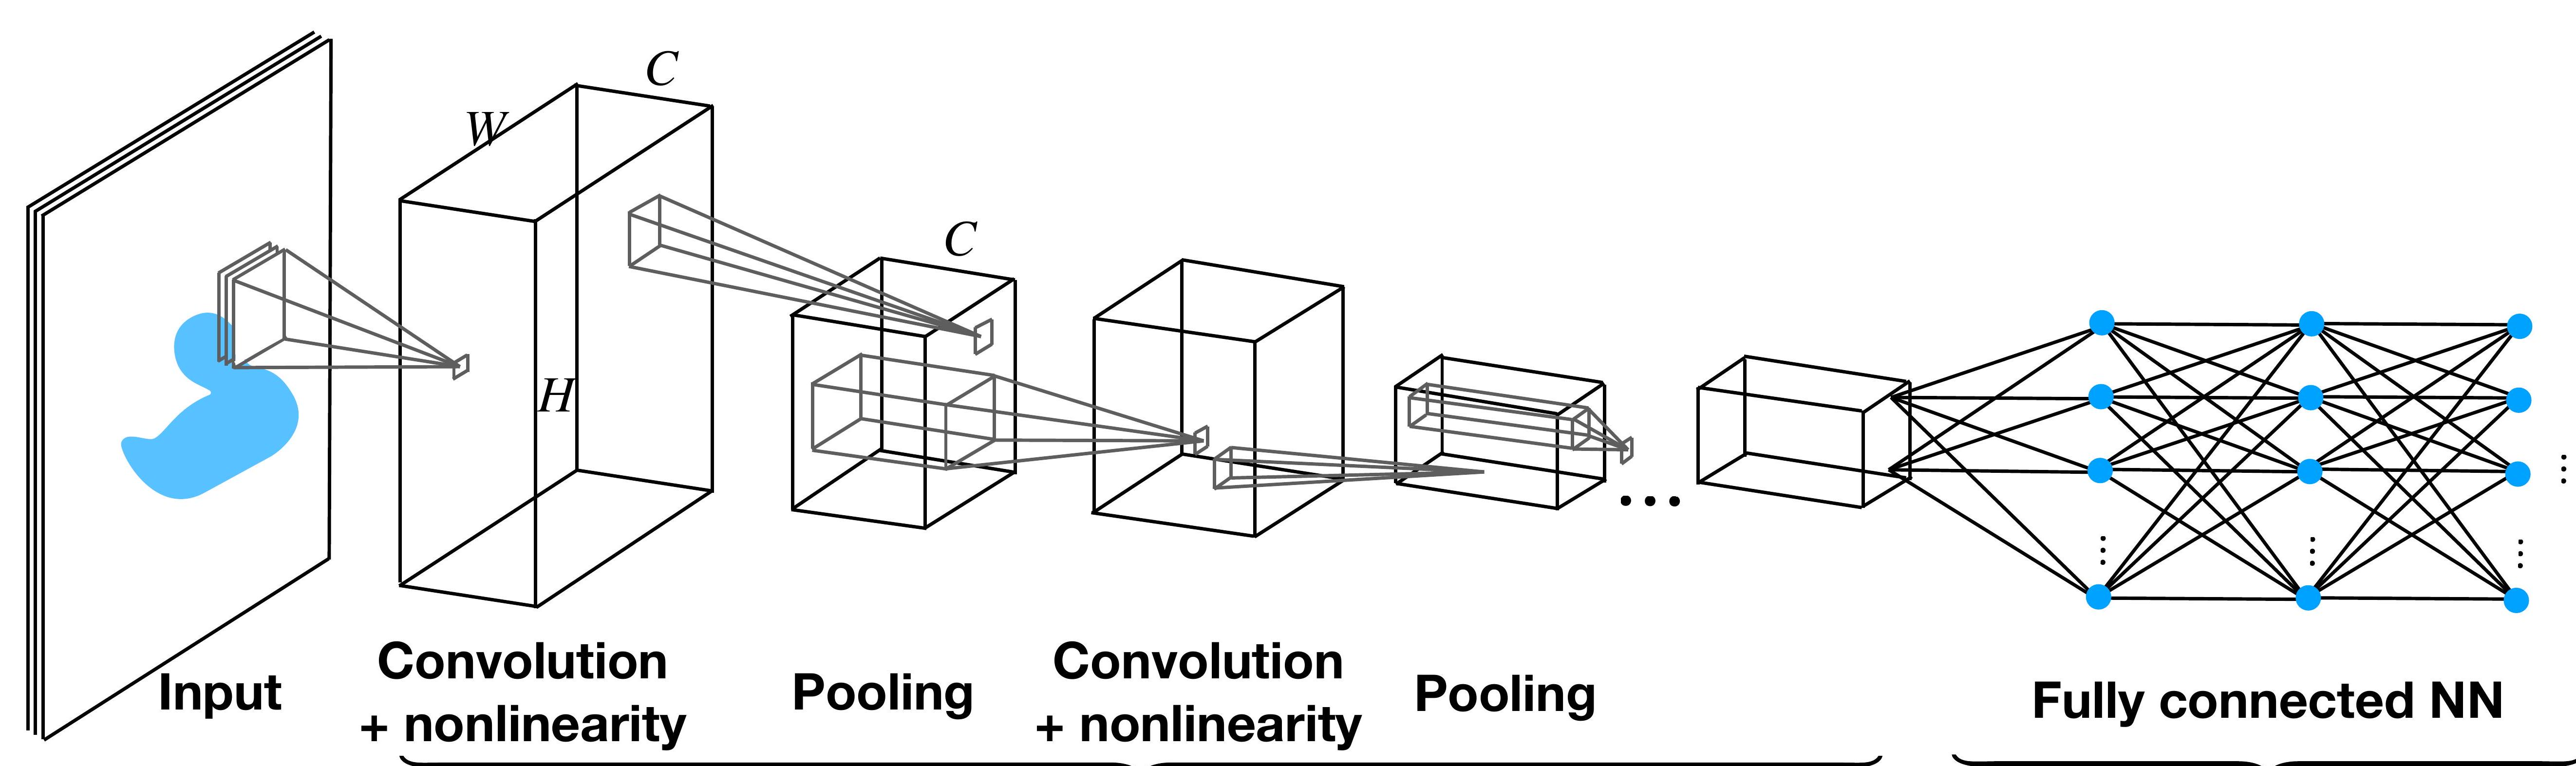
\includegraphics[max width=\textwidth]{2024_01_08_959e2db67a31f073f6d2g-12}
\end{center}

Feature Learning

Classification

Receptive field (area of input that affects a given neuron) increases with depth:

\begin{itemize}
  \item First layers extract low-level features, e.g., edges, colors
  \item Subsequent layers extract high-level features, e.g., objects
\end{itemize}

$\Rightarrow$ ConvNet reduces the images to a form easier to process without losing essential features

\section*{Backpropagation with weight sharing}
Weight sharing is used in CNN: many edges use the same weights

\section*{Training:}
\begin{enumerate}
  \item Run backpropagation as if the weights were not shared (treat each weight as an independent variable)

  \item Once the gradient is computed, sum the gradients of all edges that share the same weight

\end{enumerate}

Why: let $f(x, y, z): \mathbb{R}^{3} \rightarrow \mathbb{R}$ and $g(x, y)=f(x, y, x)$

$$
\left(\frac{\partial g}{\partial x}(x, y), \frac{\partial g}{\partial y}(x, y)\right) \underset{\prod_{\text {Chain rule }}}{=}\left(\frac{\partial f}{\partial x}(x, y, x)+\frac{\partial f}{\partial z}(x, y, x), \frac{\partial f}{\partial y}(x, y, x)\right)
$$

\section*{What do ConvNets learn?}
\section*{Learned Convolutional Filters on MNIST}
Linear model

parameter vector $w$

\begin{center}
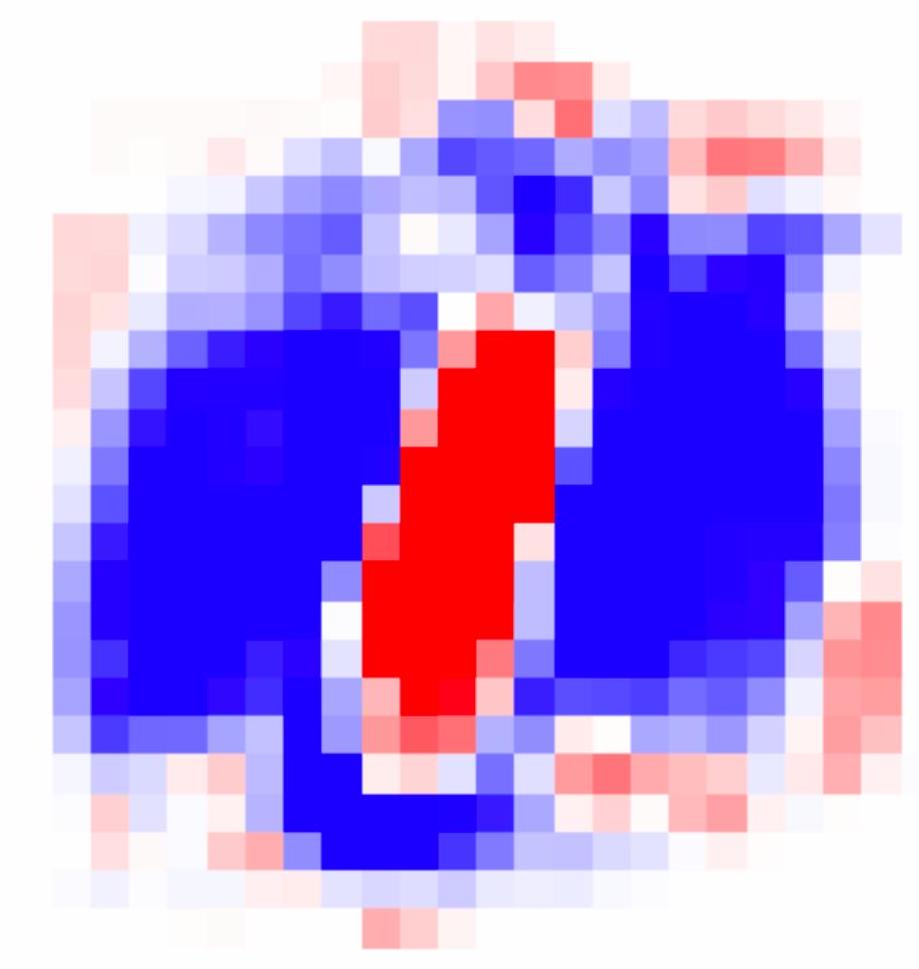
\includegraphics[max width=\textwidth]{2024_01_08_959e2db67a31f073f6d2g-15(4)}
\end{center}

Fully-connected network

\begin{center}
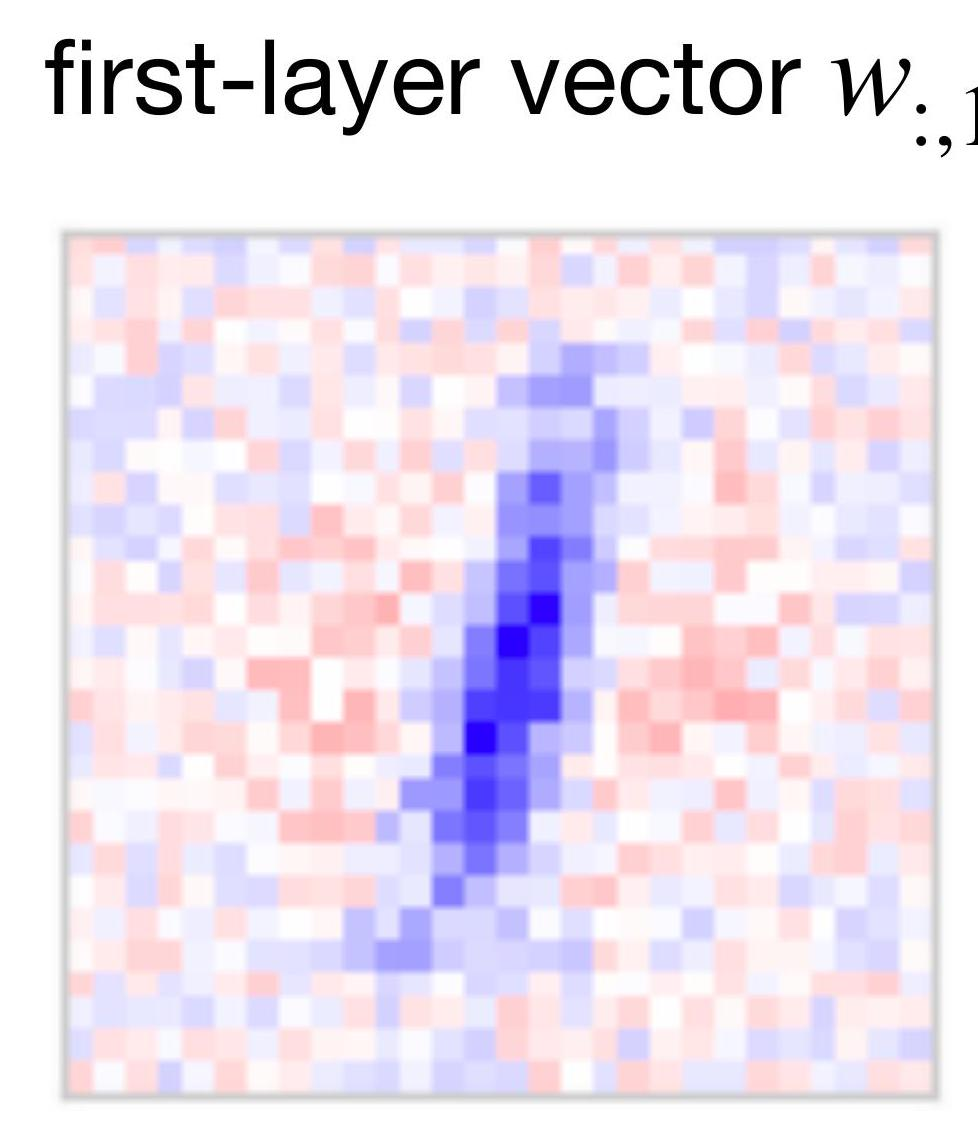
\includegraphics[max width=\textwidth]{2024_01_08_959e2db67a31f073f6d2g-15(5)}
\end{center}

first-layer vector $w_{:, 2}$

\begin{center}
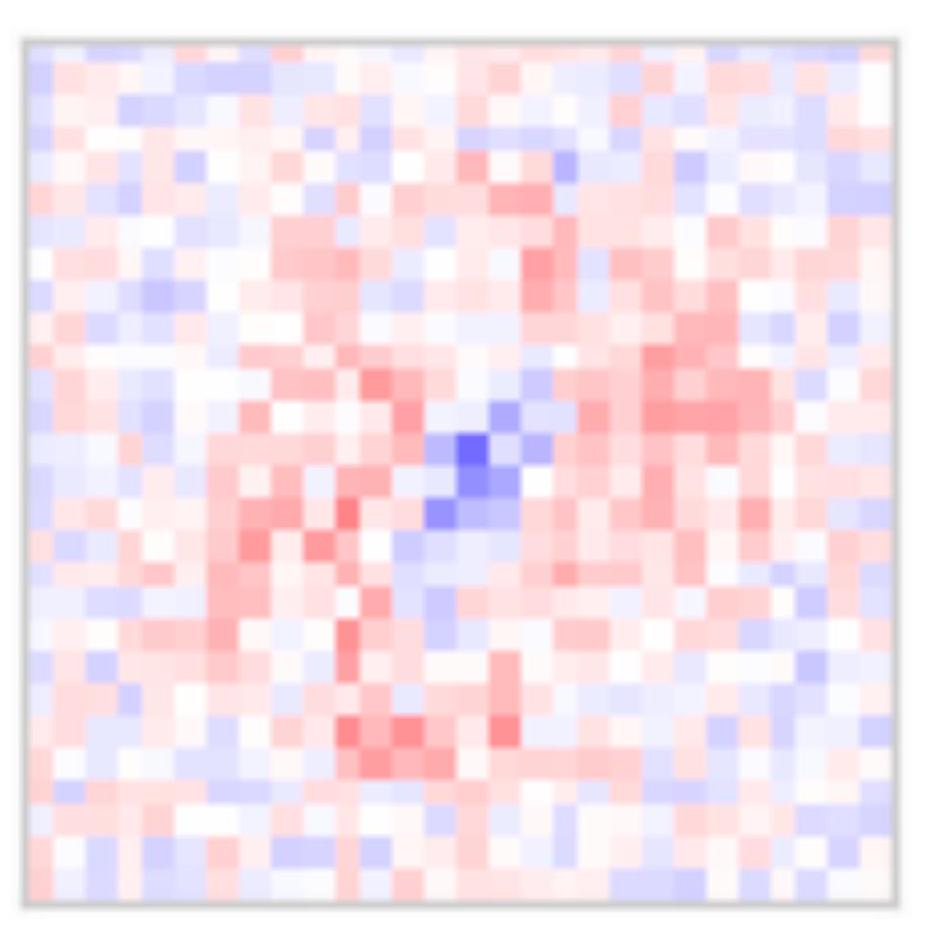
\includegraphics[max width=\textwidth]{2024_01_08_959e2db67a31f073f6d2g-15(2)}
\end{center}

first-layer vector $w_{:, 3}$

\begin{center}
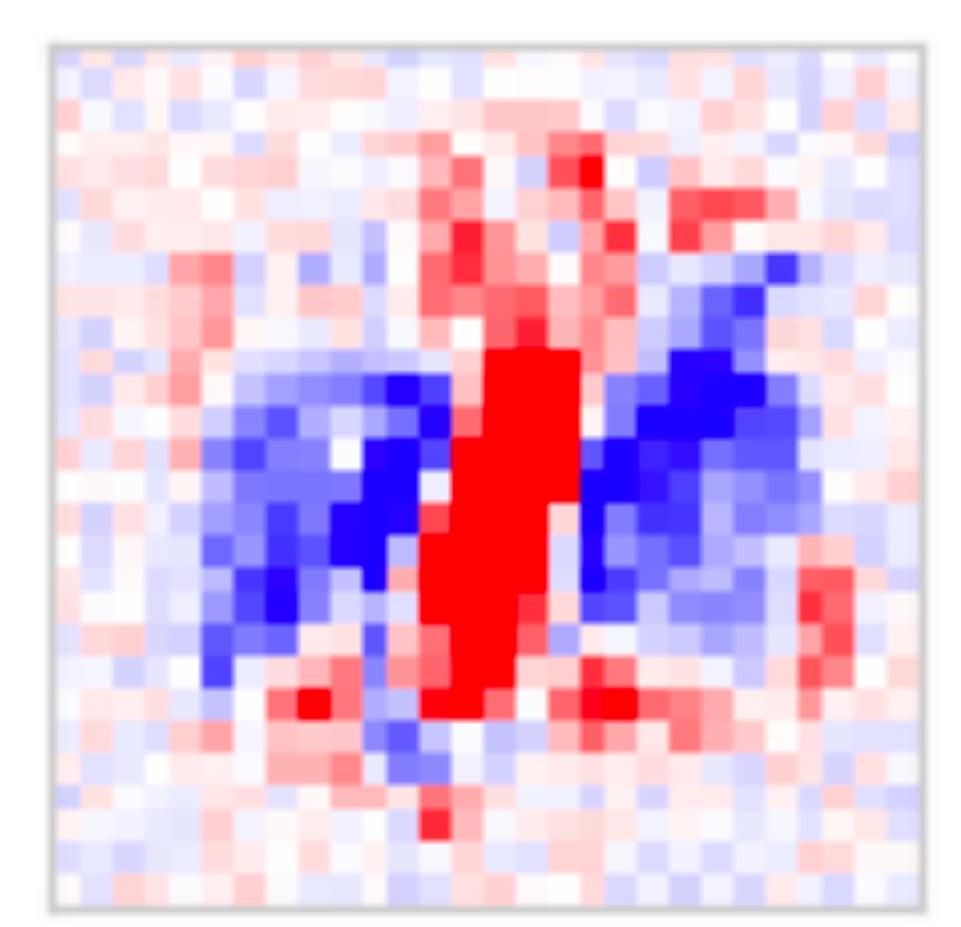
\includegraphics[max width=\textwidth]{2024_01_08_959e2db67a31f073f6d2g-15(1)}
\end{center}

first-layer vector $w_{:, 4}$

\begin{center}
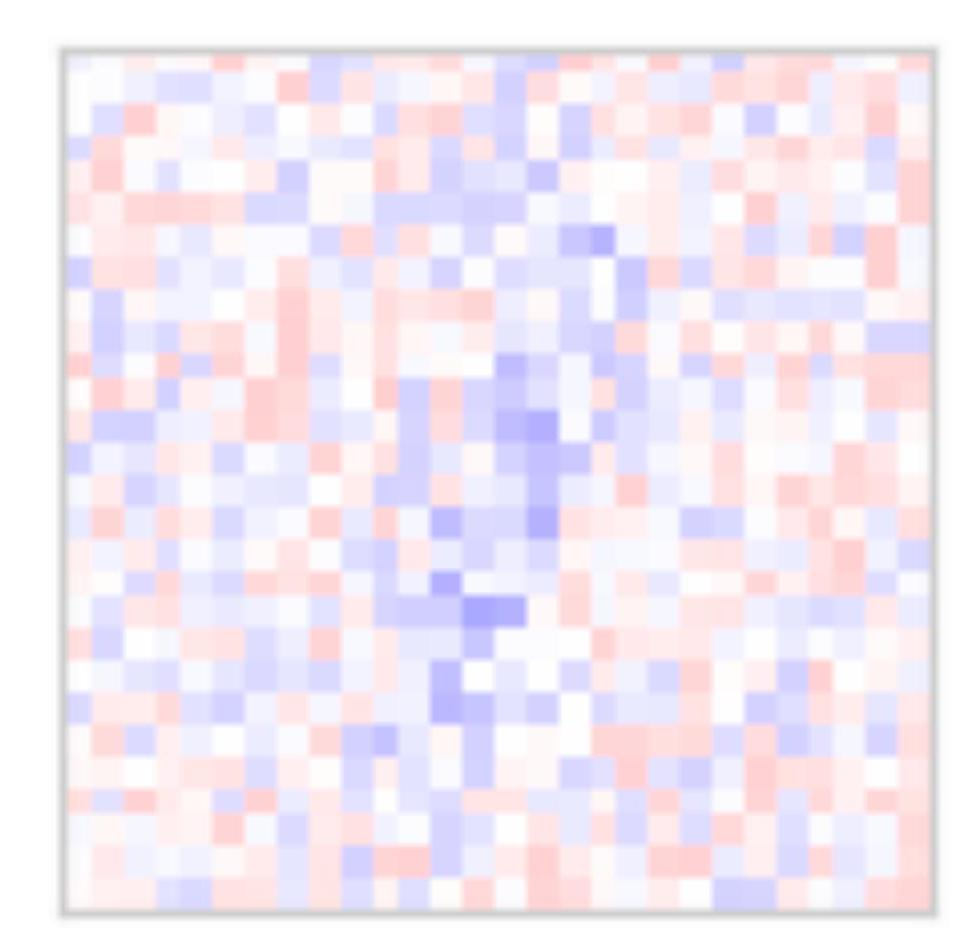
\includegraphics[max width=\textwidth]{2024_01_08_959e2db67a31f073f6d2g-15}
\end{center}

\section*{Convolutional networks}
\begin{center}
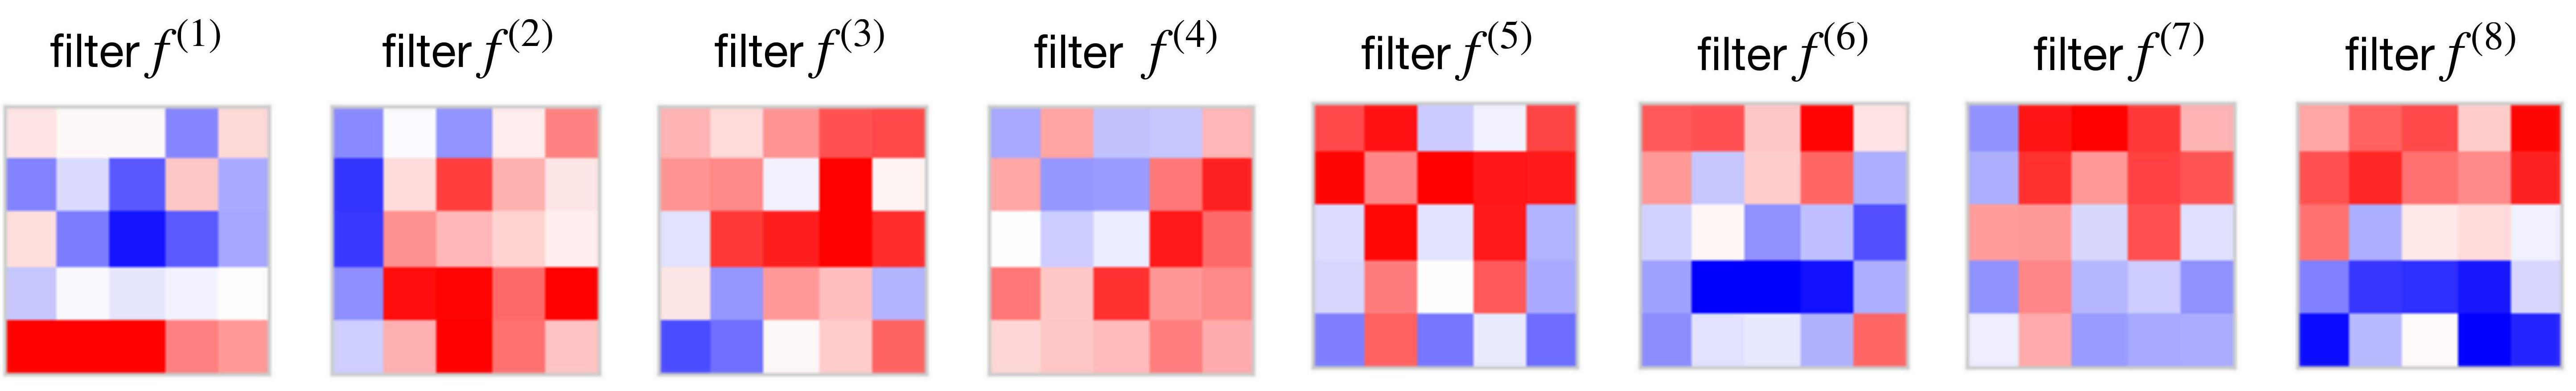
\includegraphics[max width=\textwidth]{2024_01_08_959e2db67a31f073f6d2g-15(3)}
\end{center}

\section*{Learned Convolutional Filters on ImageNet}
\begin{center}
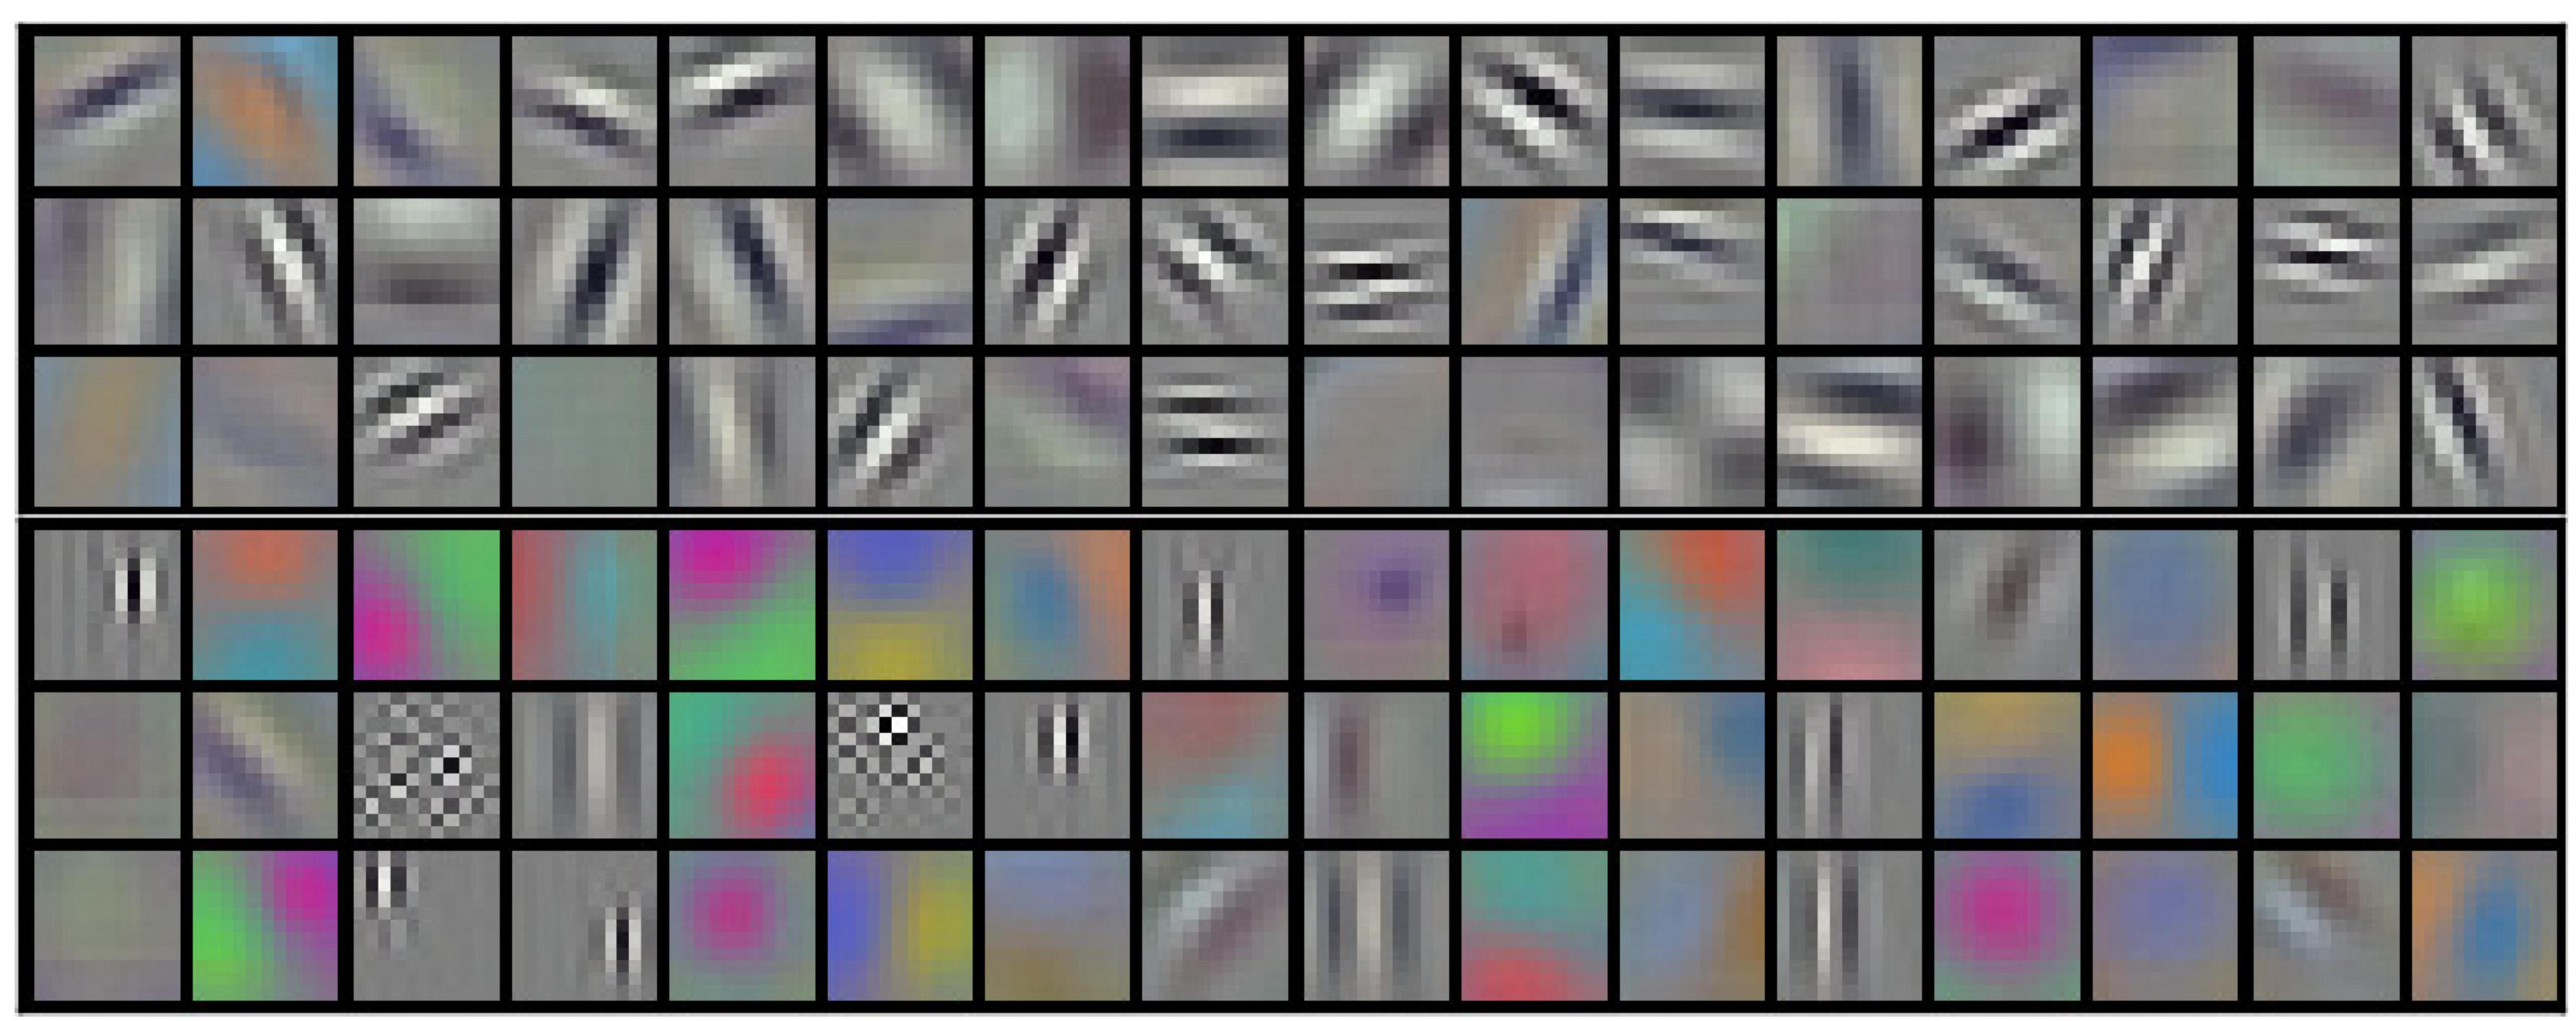
\includegraphics[max width=\textwidth]{2024_01_08_959e2db67a31f073f6d2g-16}
\end{center}

Source: ImageNet Classification with Deep Convolutional Neural Networks (NeurIPS 2012)

\begin{itemize}
  \item Filters of the first layer can be interpretable

  \item Edge and color detectors typically emerge when trained on large datasets

\end{itemize}

\section*{Individual Activations Can Be Interpretable}
\begin{center}
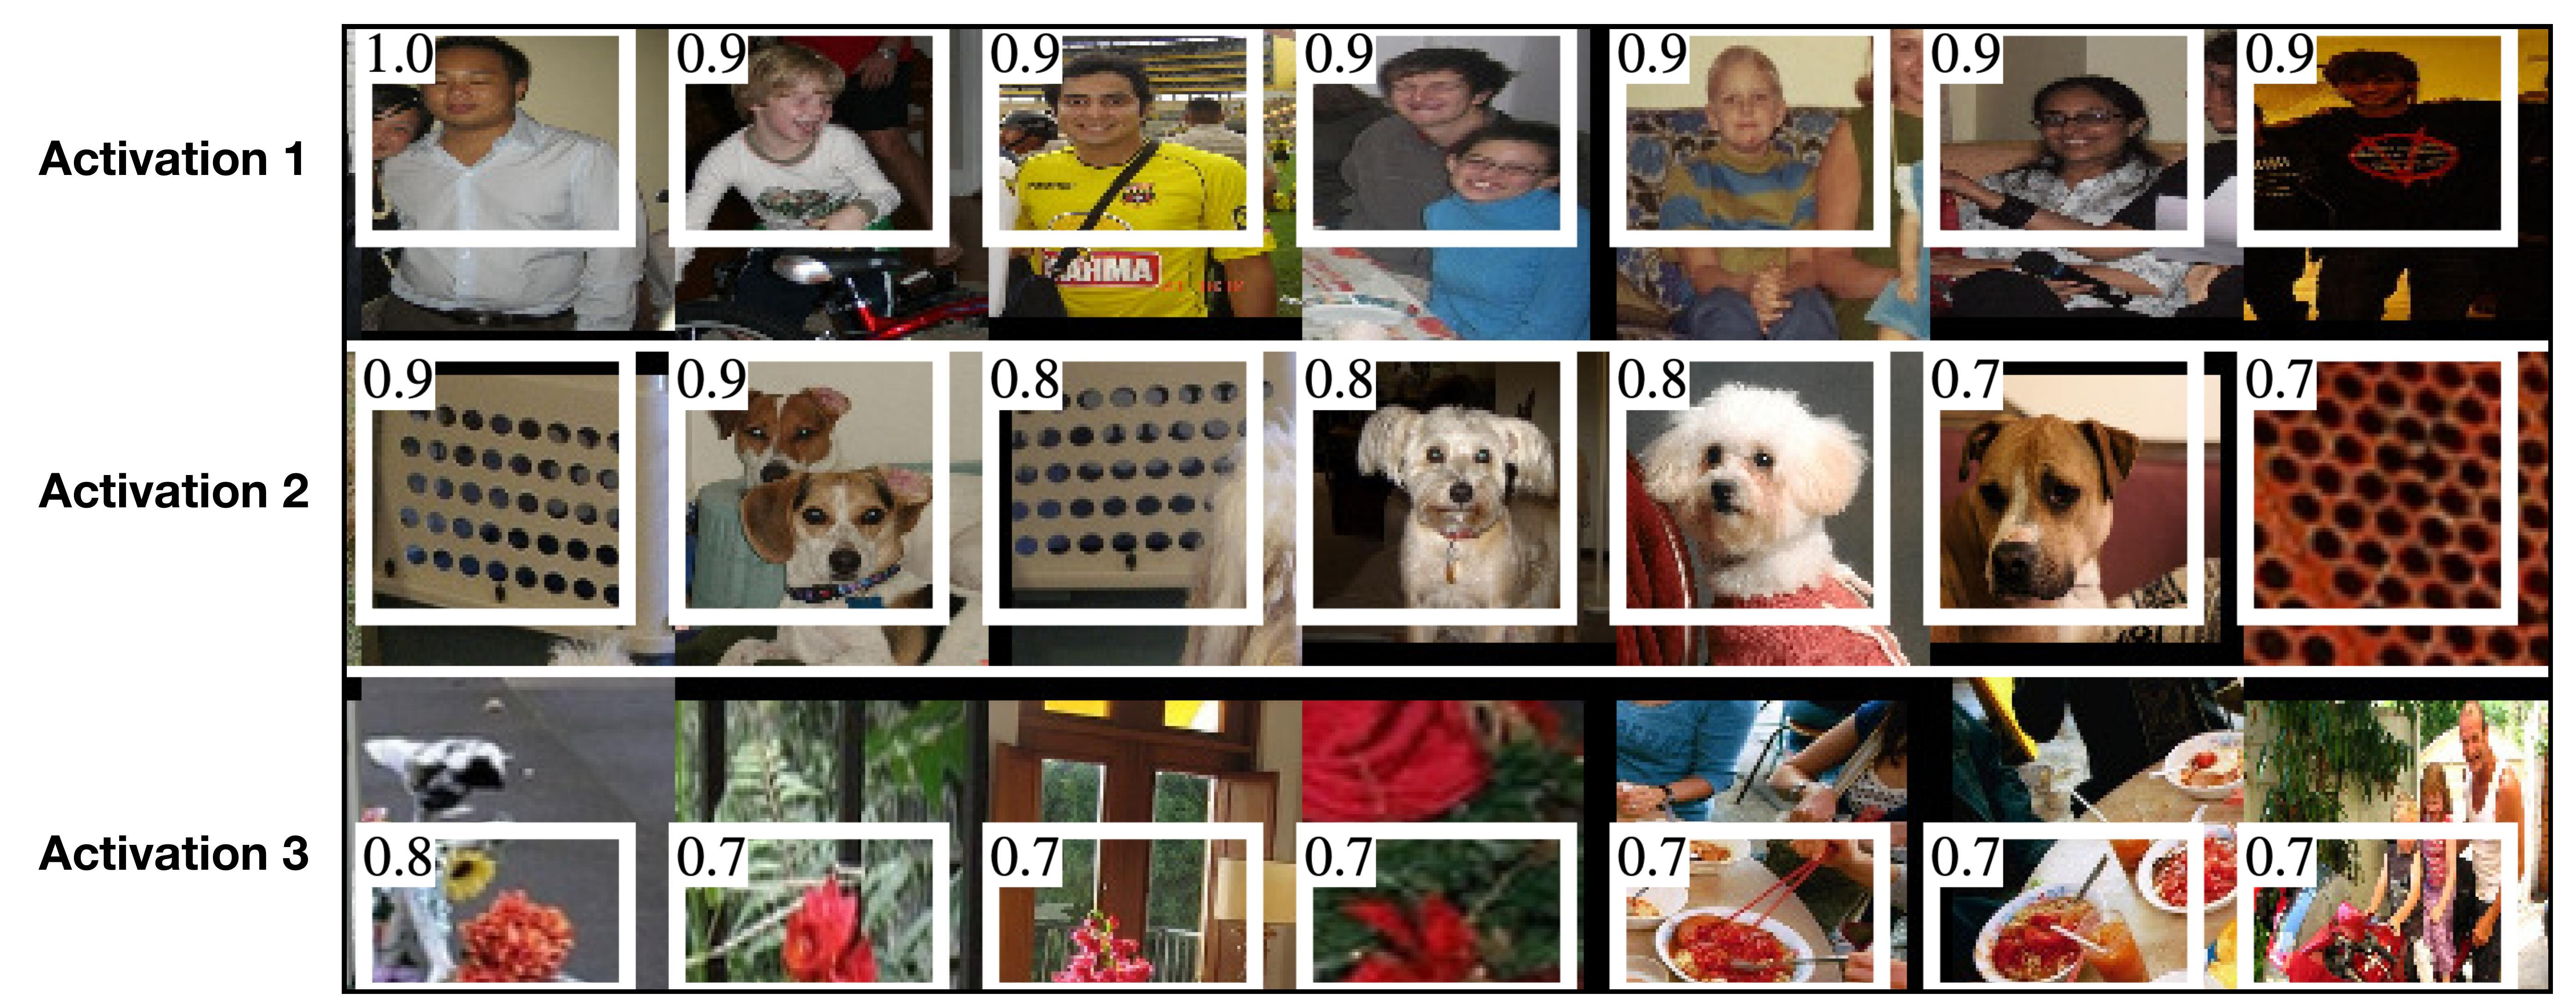
\includegraphics[max width=\textwidth]{2024_01_08_959e2db67a31f073f6d2g-17}
\end{center}

Source: Rich feature hierarchies for accurate object detection and semantic segmentation (CVPR 2014)

\begin{itemize}
  \item Receptive fields and activation values are drawn in white
  \item Each activation detects some pattern or object (not always interpretable)
  \item Activations in later layers detect more complex patterns
\end{itemize}

\section*{Residual Networks}
\section*{Skip Connections and Residuals}
\begin{itemize}
  \item Starting point: Adding more layers should lead to the same or lower training loss as they can learn the identity function

  \item ResNet paper indicates that this is not always the case

  \item Solution: add a skip connection around some layers $F(\mathbf{X})$

  \item Standard network: $\mathbf{Y}=F(\mathbf{X})$

  \item Residual network: $\mathbf{Y}=R(\mathbf{X})+\mathbf{X}$ where $R(\mathbf{X})$ is called a residual branch

\end{itemize}

\begin{center}
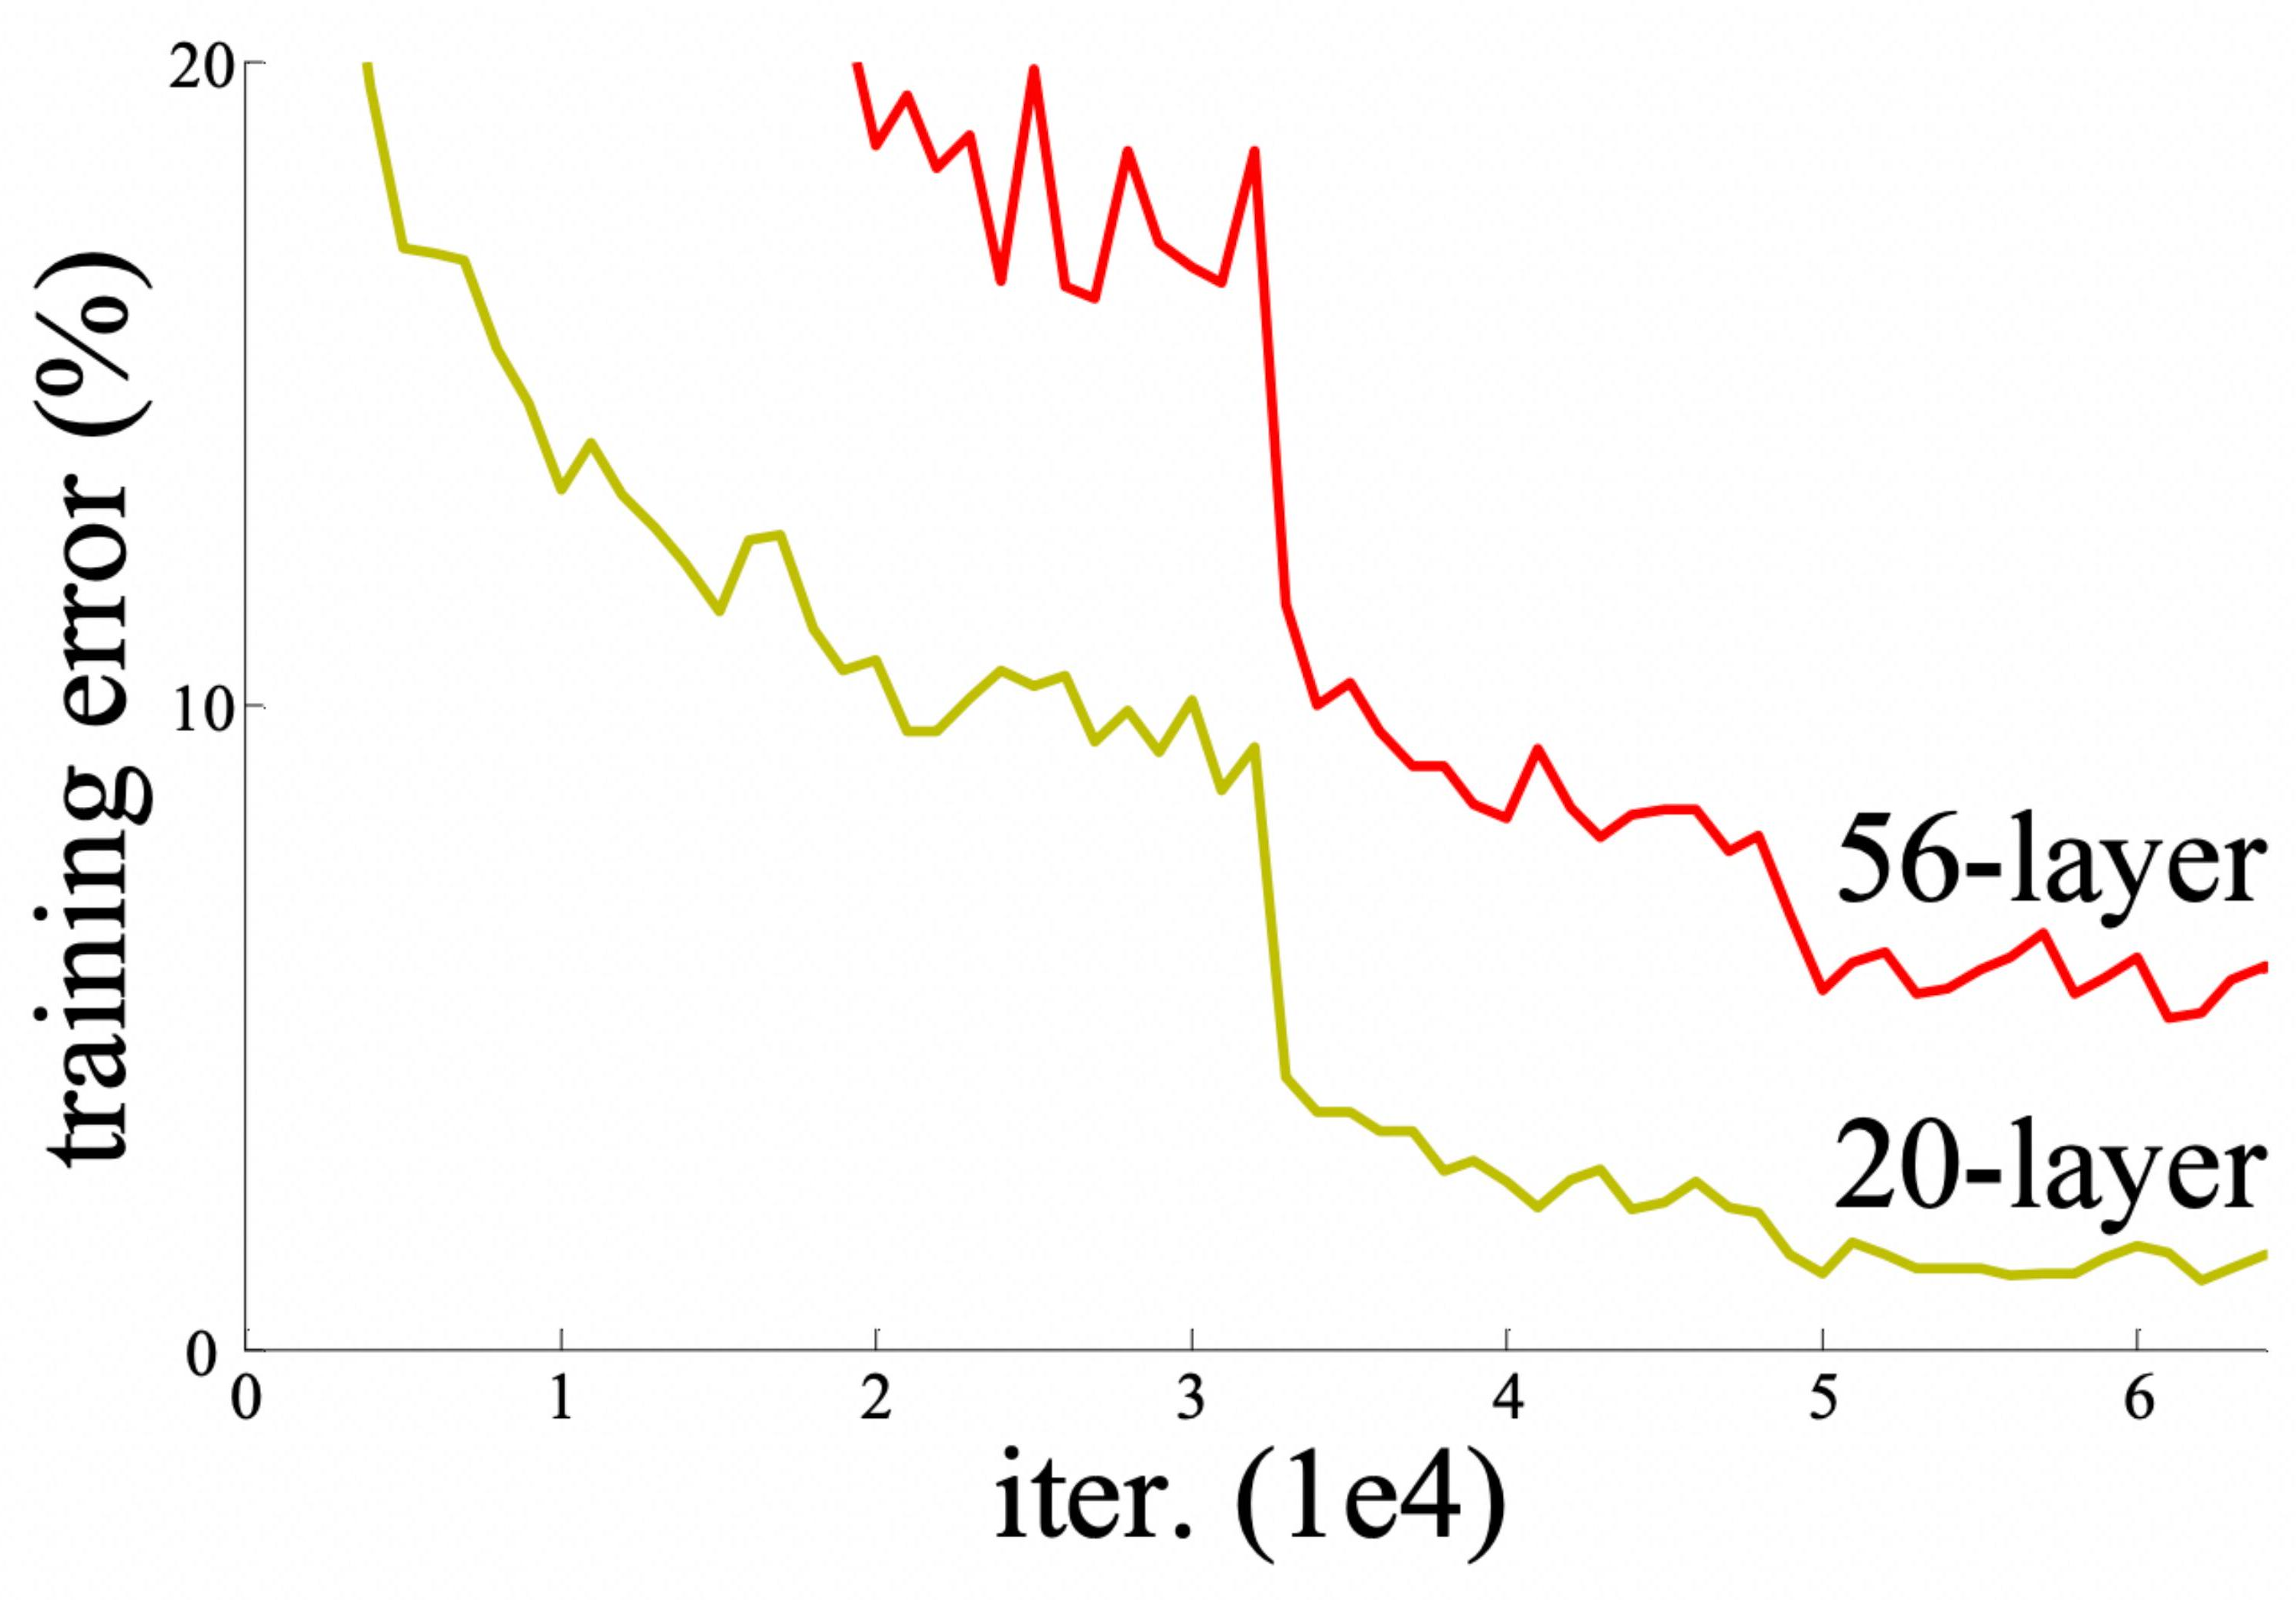
\includegraphics[max width=\textwidth]{2024_01_08_959e2db67a31f073f6d2g-19}
\end{center}

Observation from the ResNet paper: deeper CNNs are harder to train

\section*{Skip Connections and Residuals}
\begin{itemize}
  \item Example of $R(\mathbf{X})$ : see on the right

  \item Technical detail: If $\operatorname{size}(\mathbf{Y}) \neq \operatorname{size}(\mathbf{X})$, additional operations are needed on the skip connection to match the dimensions

  \item Skip connections address the observed convergence issue, making the training of very deep networks (with hundreds of layers) feasible

  \item Skip connections are used in almost all modern neural networks (including CNNs and transformers)

\end{itemize}

\begin{center}
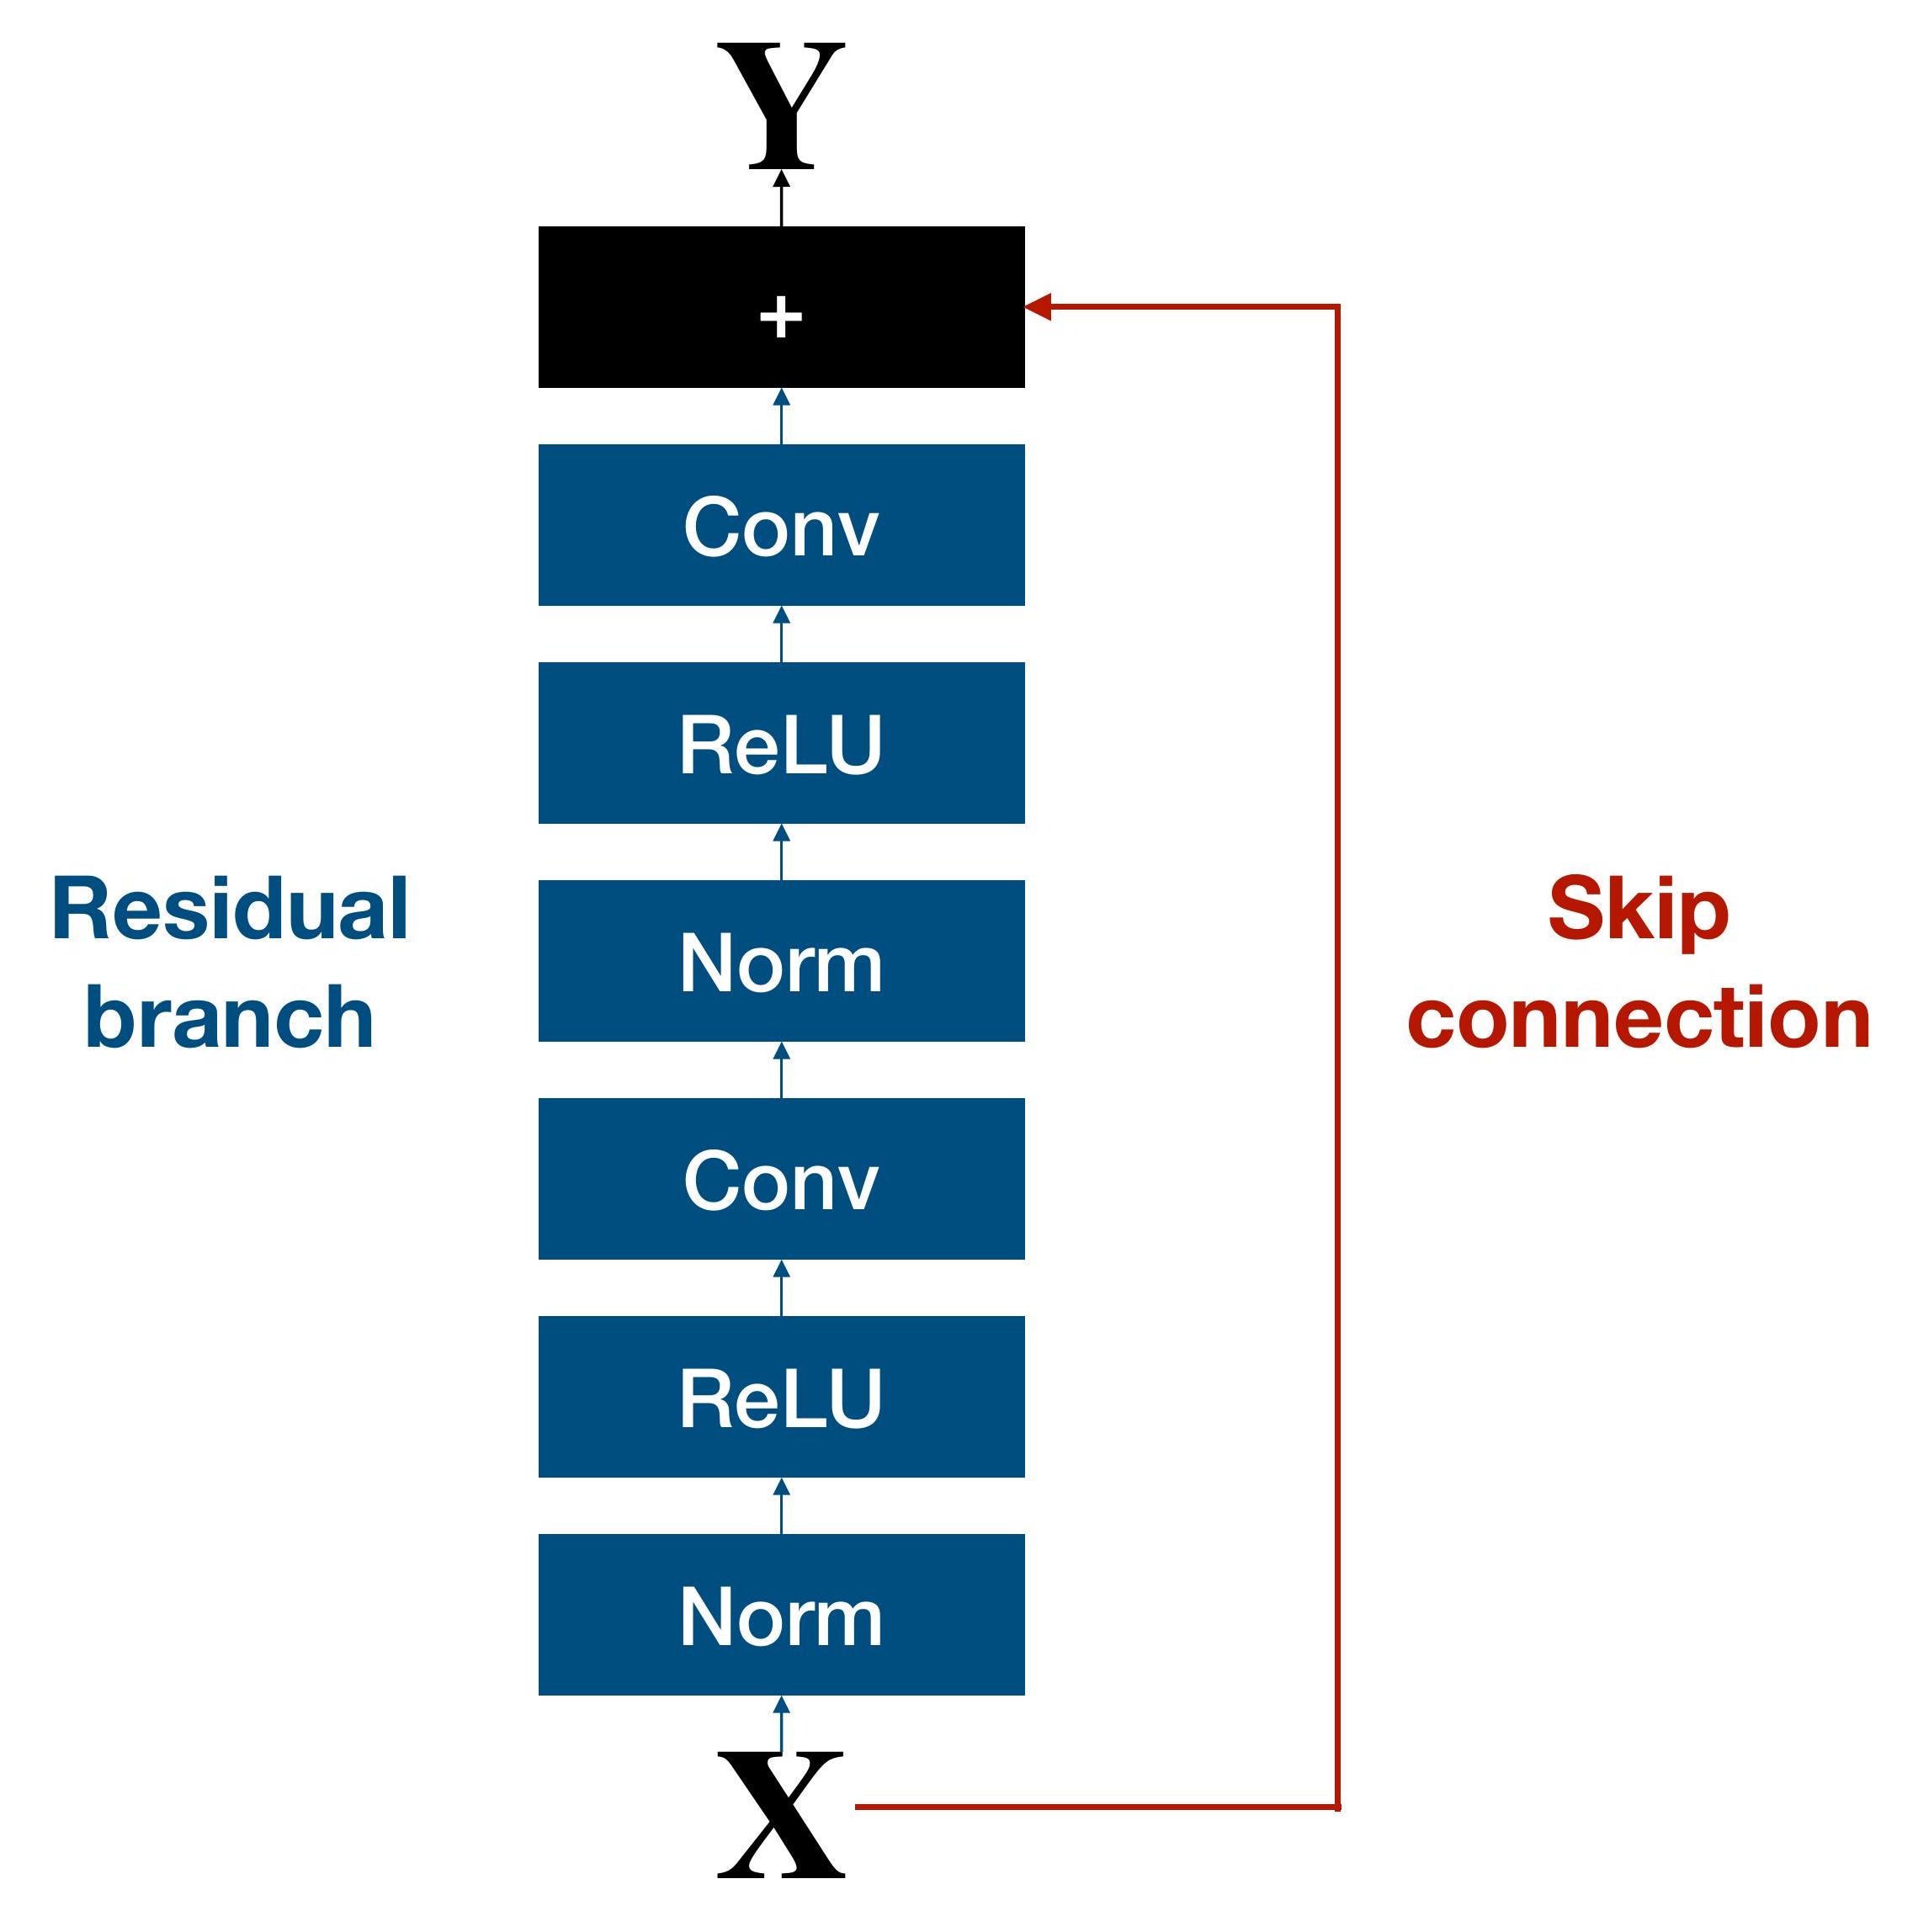
\includegraphics[max width=\textwidth]{2024_01_08_959e2db67a31f073f6d2g-20}
\end{center}

Example residual block

\section*{Popular architectures: VGG vs. ResNet}
\begin{center}
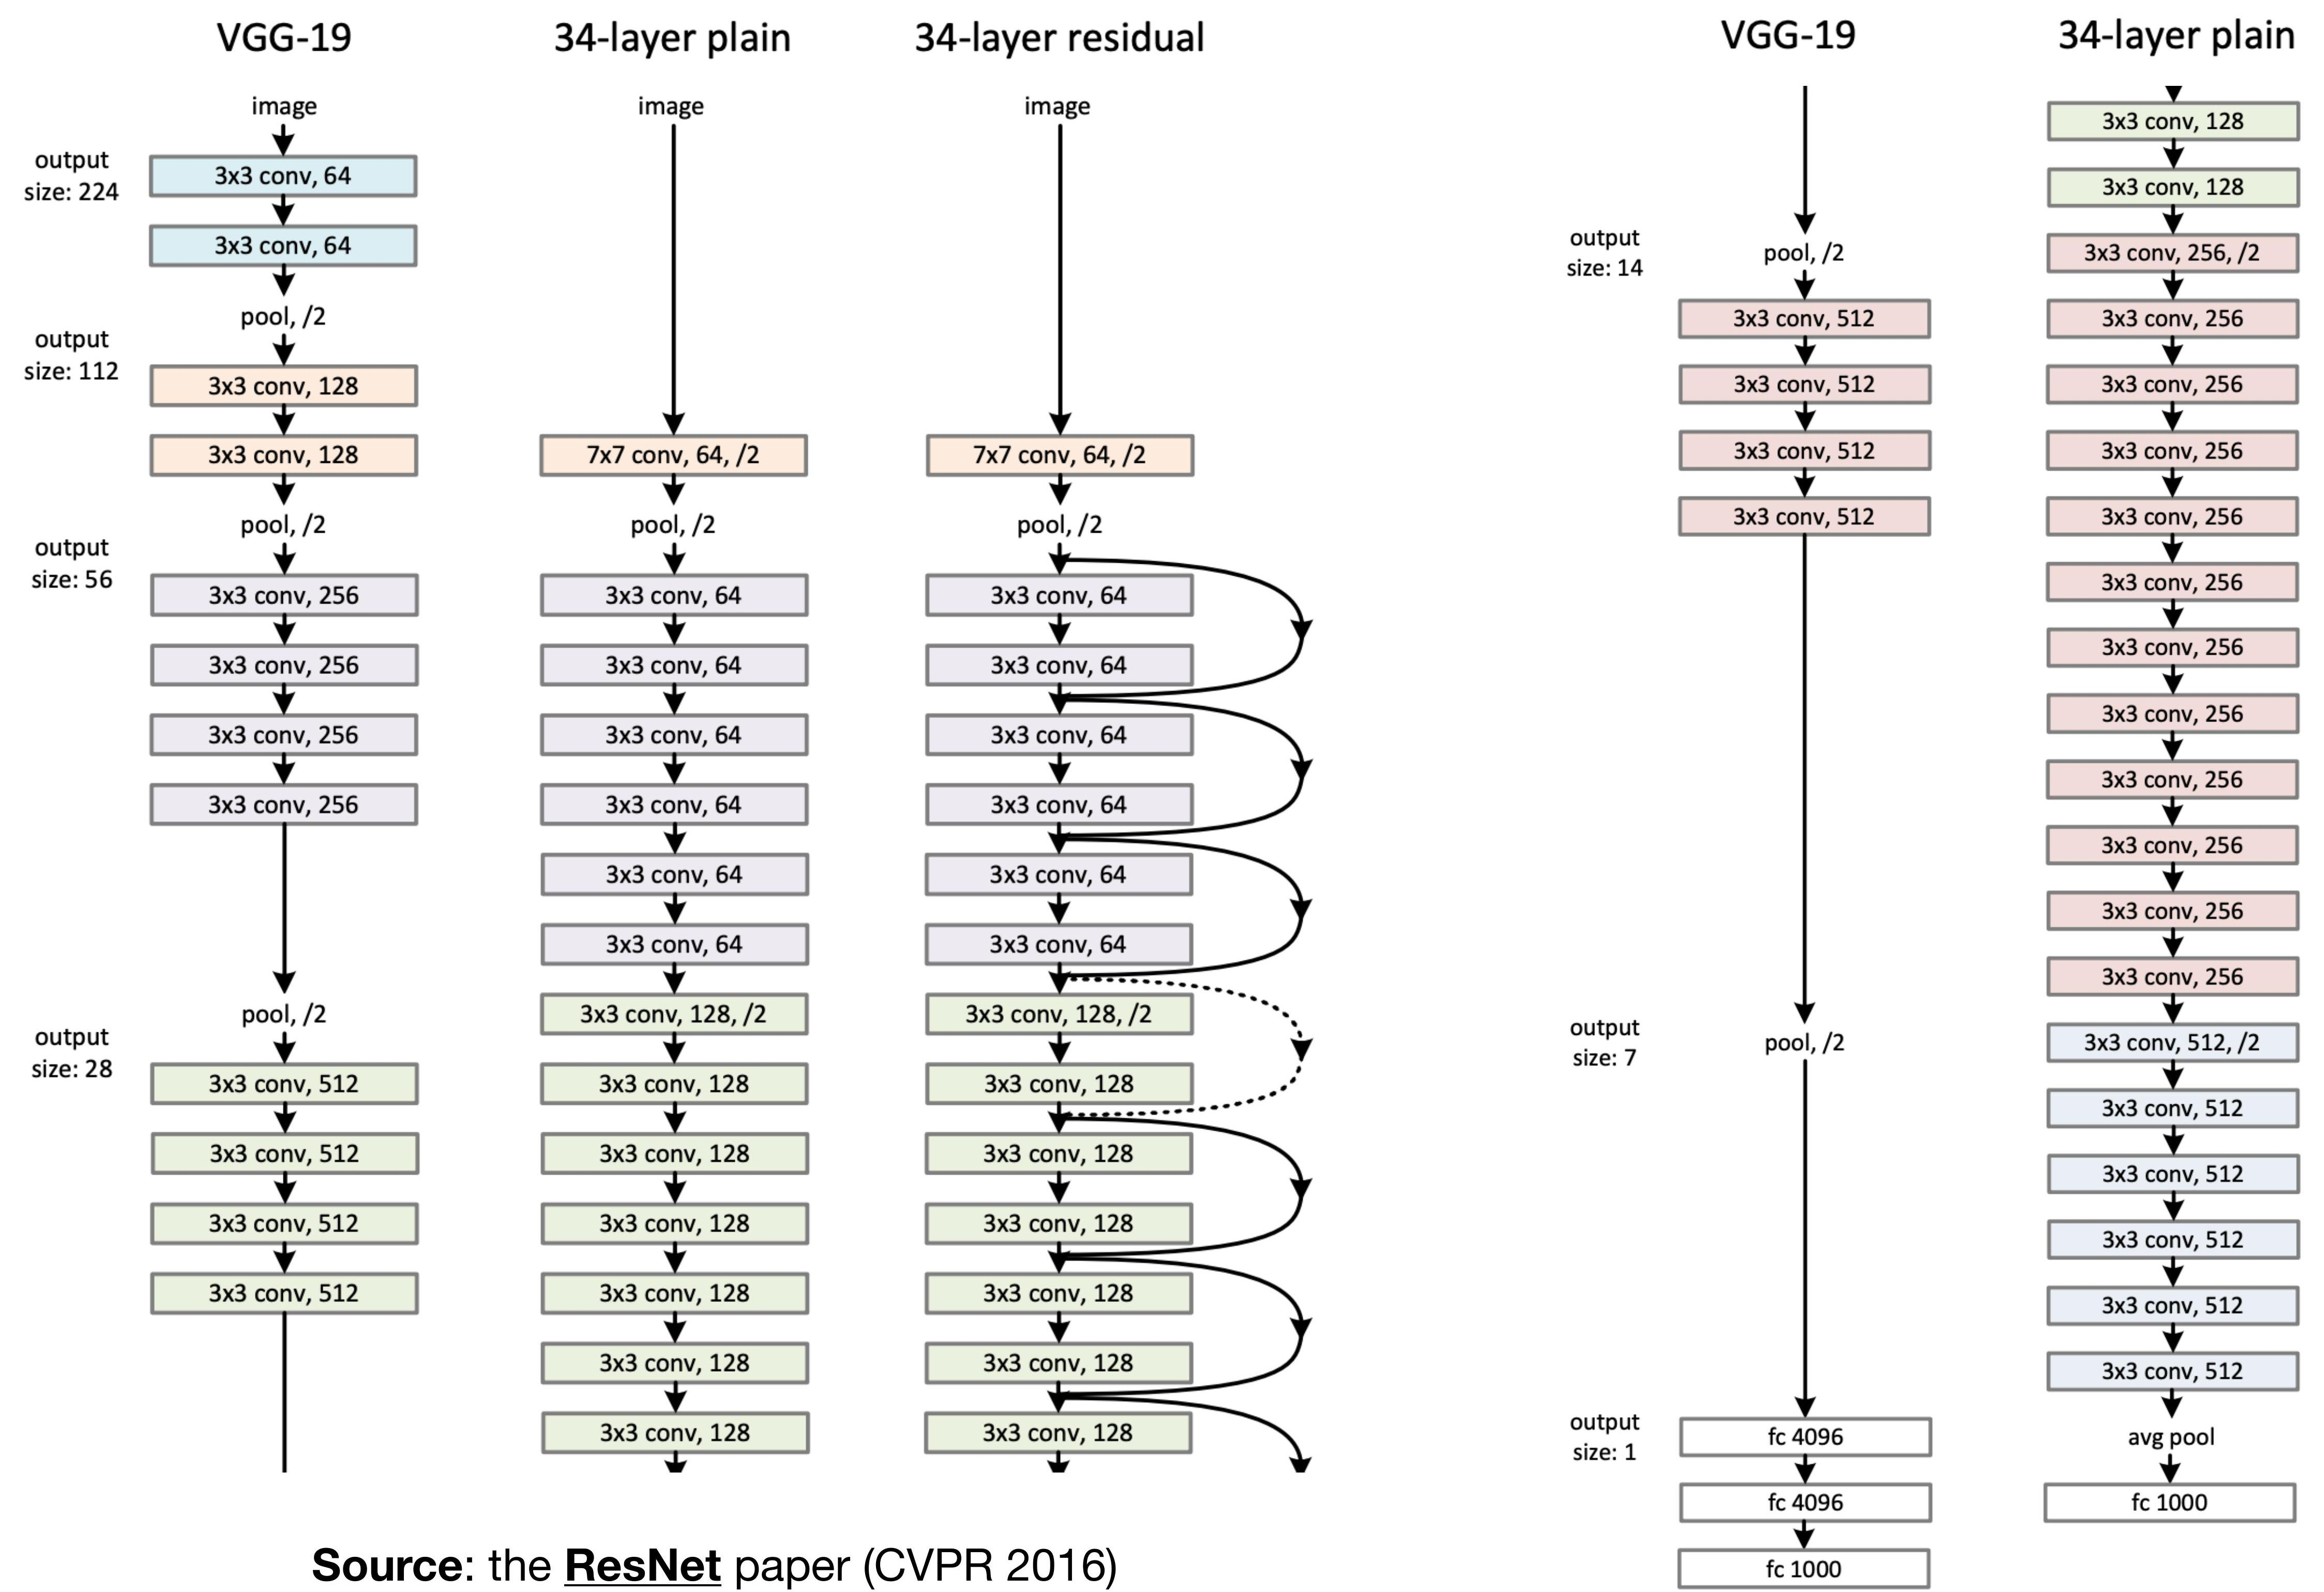
\includegraphics[max width=\textwidth]{2024_01_08_959e2db67a31f073f6d2g-21(1)}
\end{center}

34-layer residual

\begin{center}
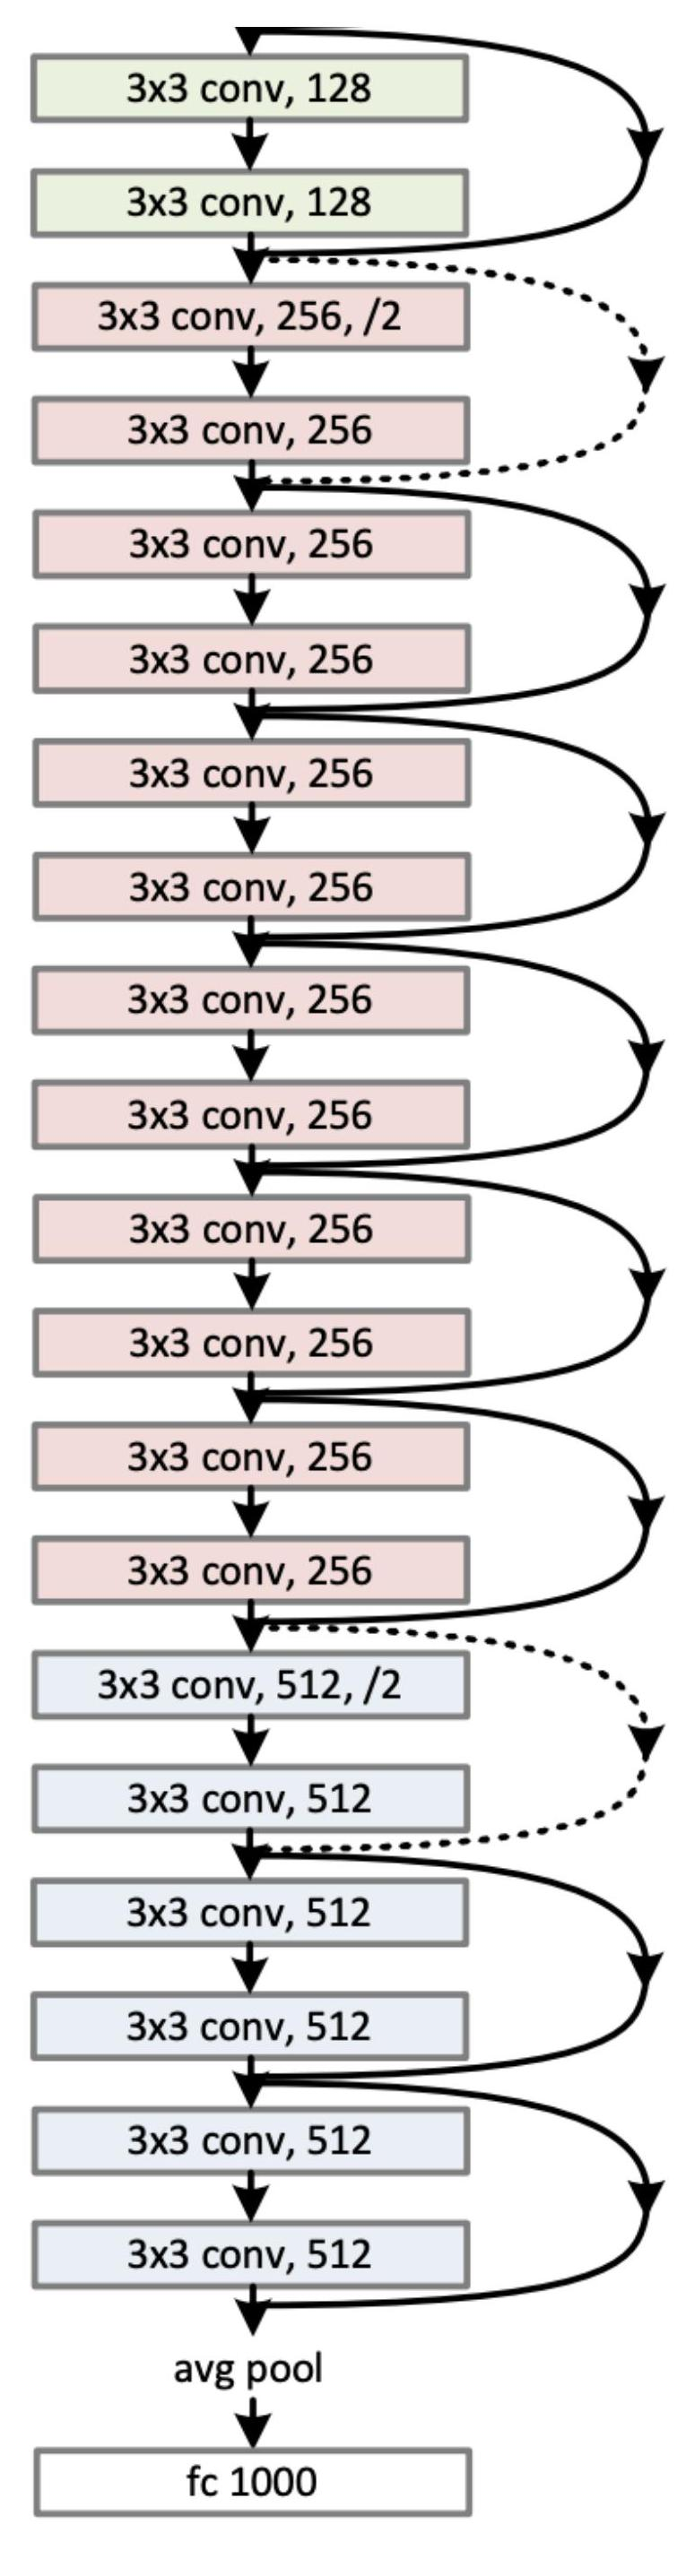
\includegraphics[max width=\textwidth]{2024_01_08_959e2db67a31f073f6d2g-21}
\end{center}

\section*{Data Augmentation}
\section*{Data augmentation: generate new data from the data}
\begin{center}
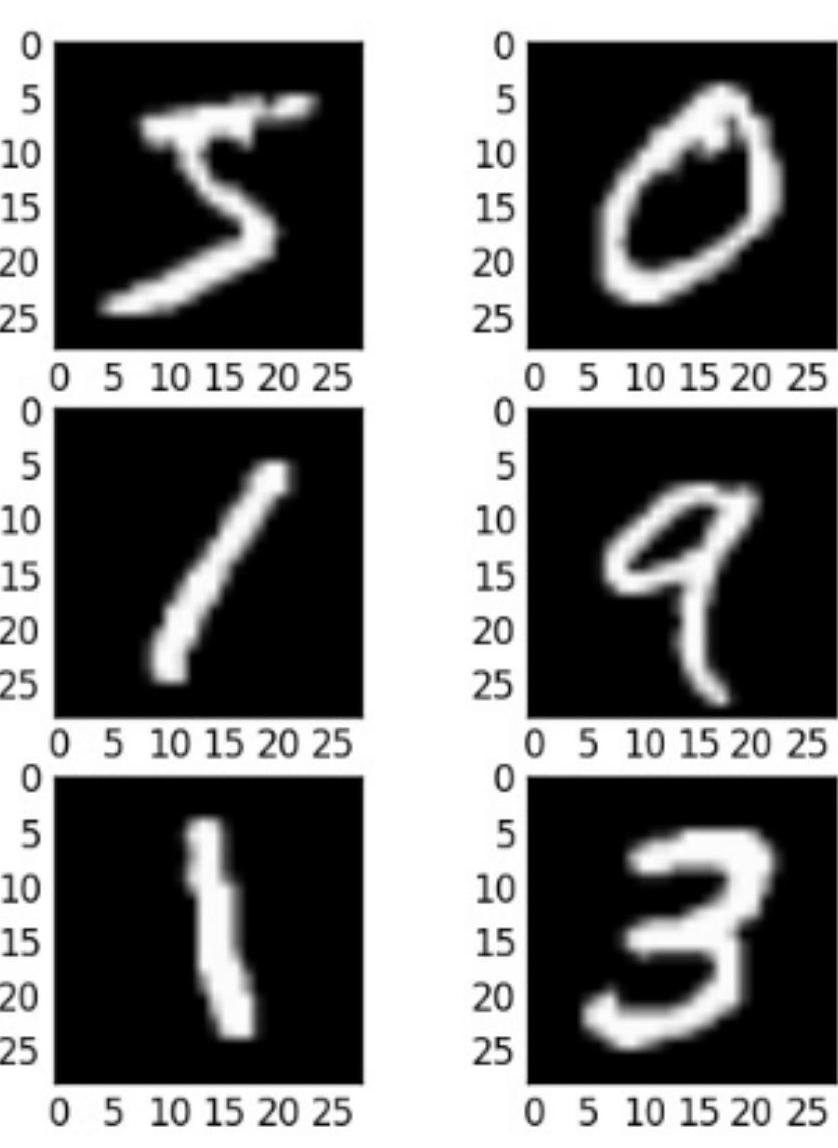
\includegraphics[max width=\textwidth]{2024_01_08_959e2db67a31f073f6d2g-23(2)}
\end{center}

MNIST

\begin{center}
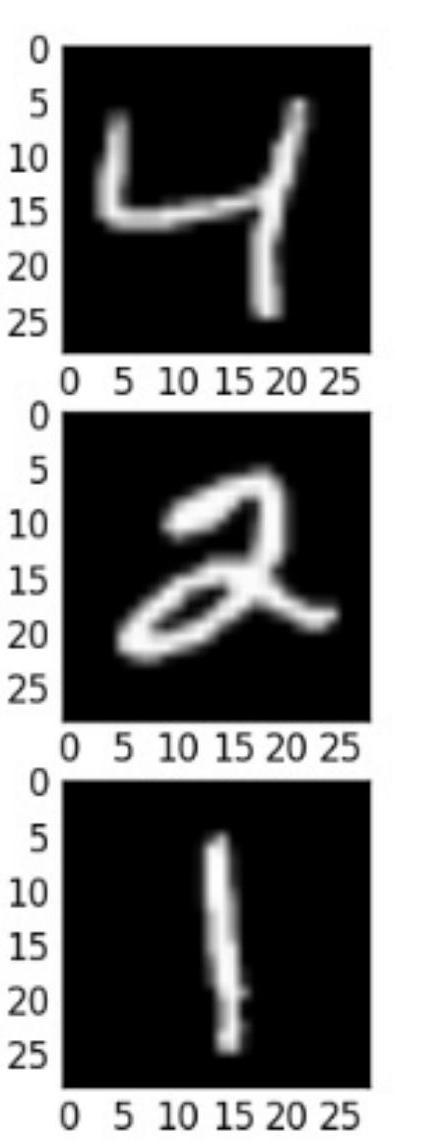
\includegraphics[max width=\textwidth]{2024_01_08_959e2db67a31f073f6d2g-23}
\end{center}

0510152025
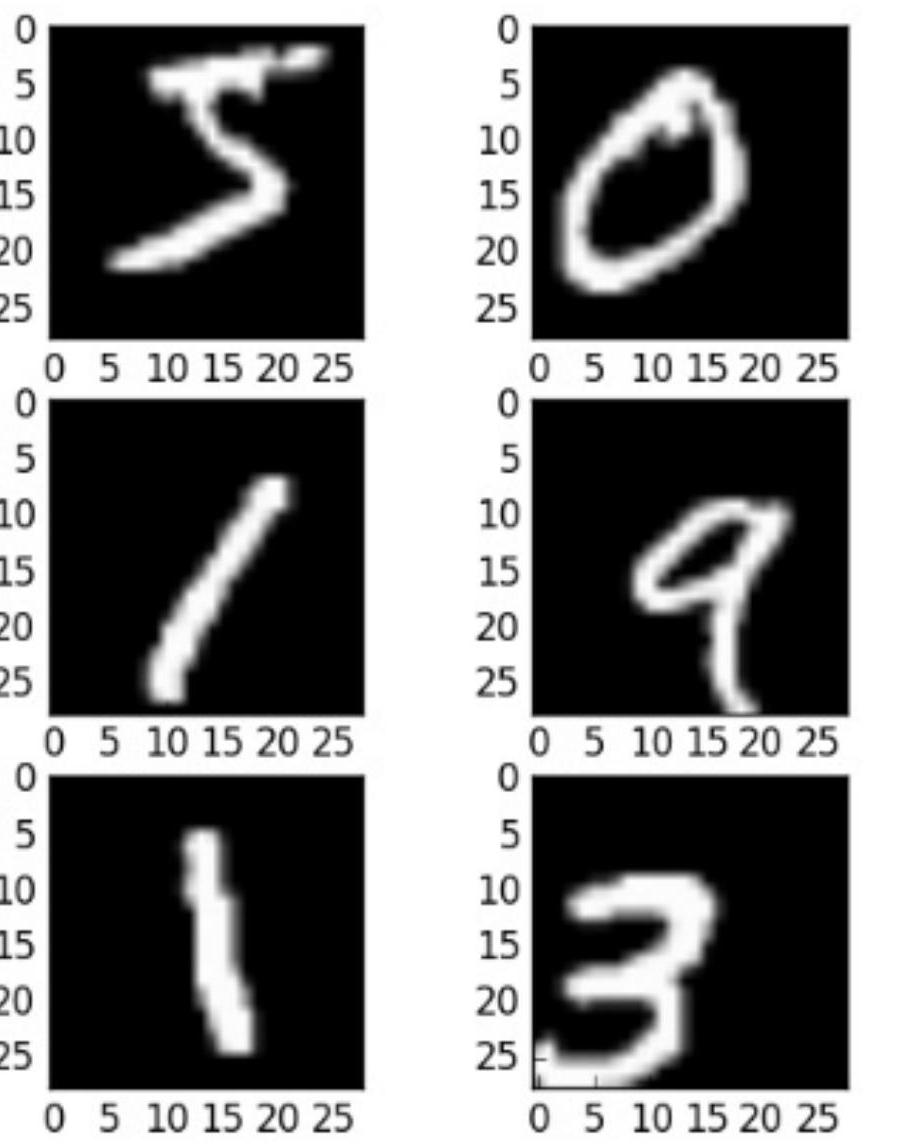
\includegraphics[max width=\textwidth, center]{2024_01_08_959e2db67a31f073f6d2g-23(1)}

Shifted MNIST
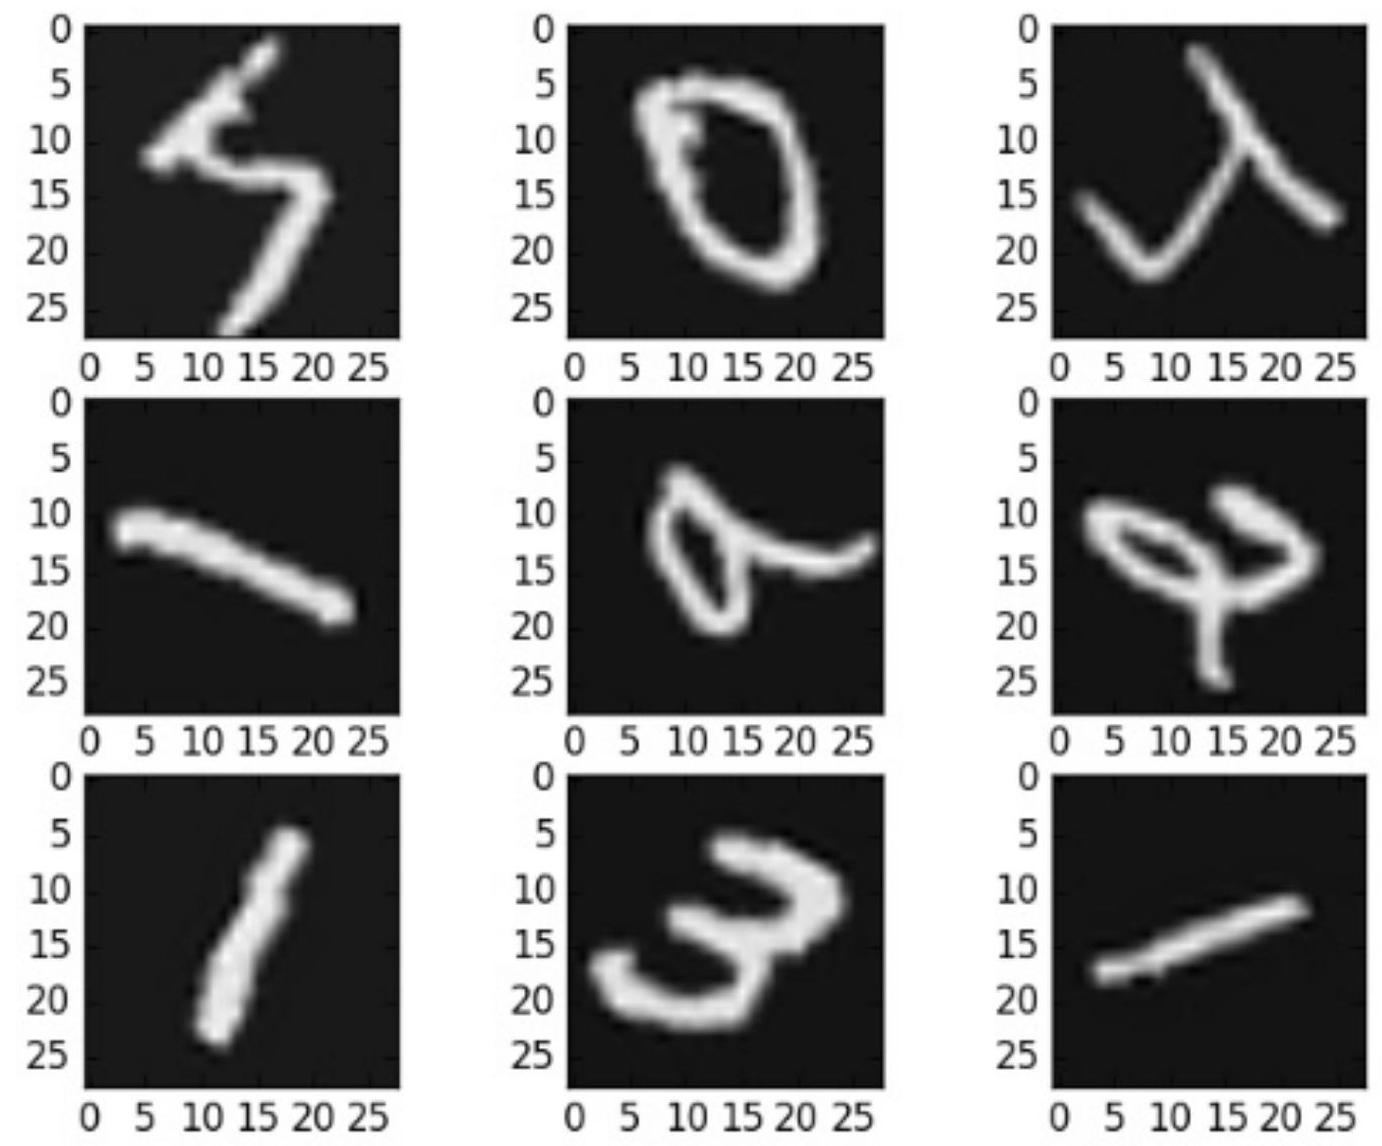
\includegraphics[max width=\textwidth, center]{2024_01_08_959e2db67a31f073f6d2g-23(3)}

Rotated MNIST
Note dangers of excessive augmentation! May eventually confuse 6 and 9

Transformation $\tau: \mathbb{R}^{d} \rightarrow \mathbb{R}^{d}$ which preserves the labels (i.e., $y_{x}=y_{\tau(x)}$ )

$$
S=S_{\text {train }} \cup\left\{\left(\tau\left(x_{i}\right), y_{i}\right)\right\}_{i=1}^{n}
$$

\begin{itemize}
  \item We train on more data

  \item Encourages models to be invariant to $\tau$

  \item It can be seen as regularization

  \item These transformations are task and dataset specific

\end{itemize}

\section*{Data augmentation: pictures can also be cropped, resized, or perturbed by a small amount of noise}
\begin{center}
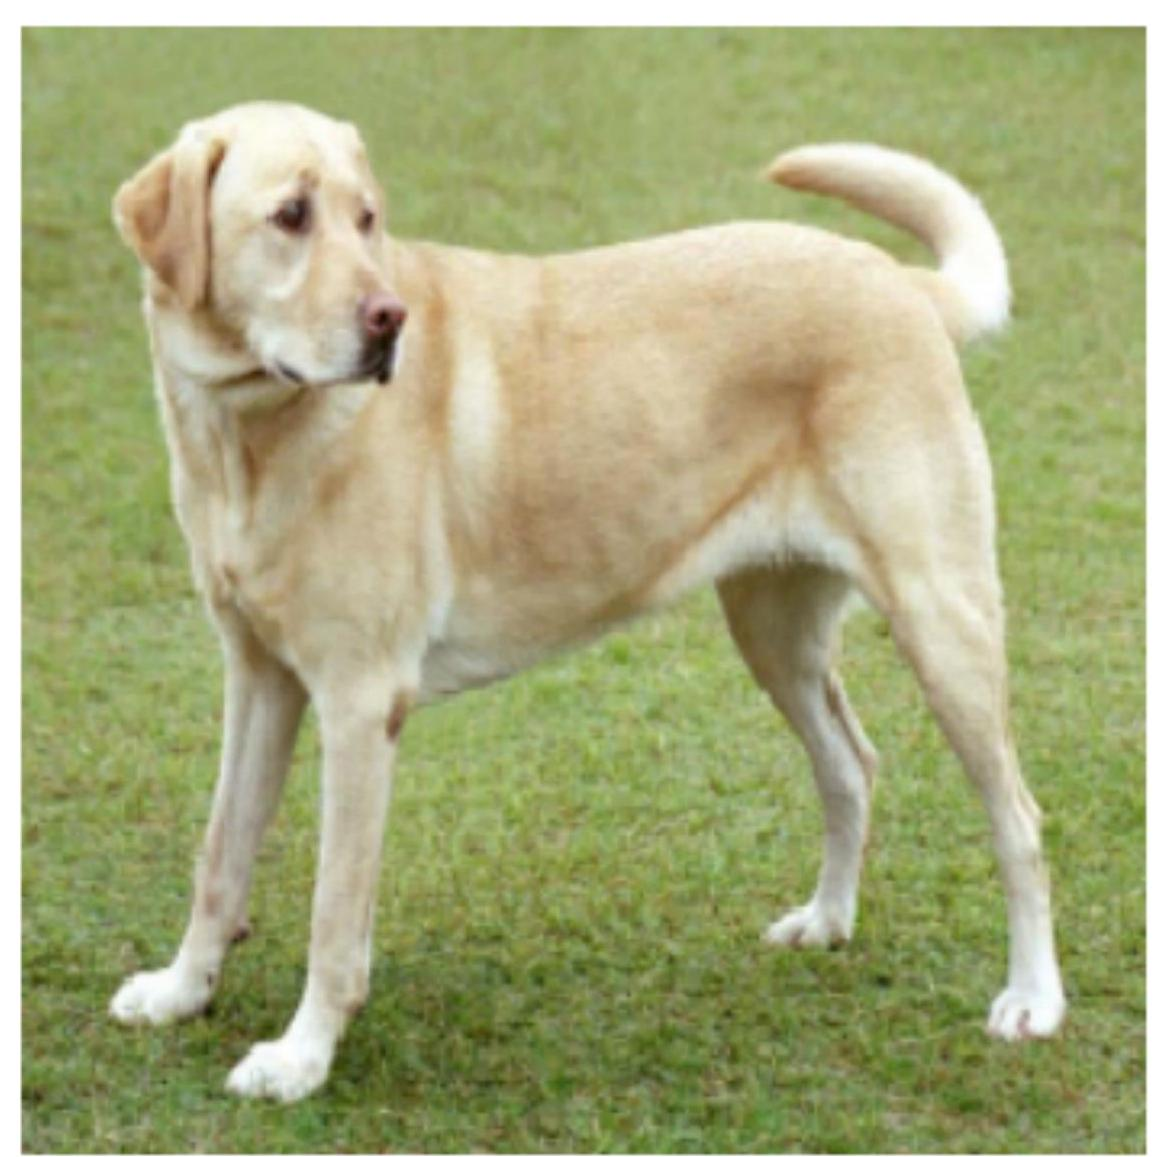
\includegraphics[max width=\textwidth]{2024_01_08_959e2db67a31f073f6d2g-24(3)}
\end{center}

(a) Original

\begin{center}
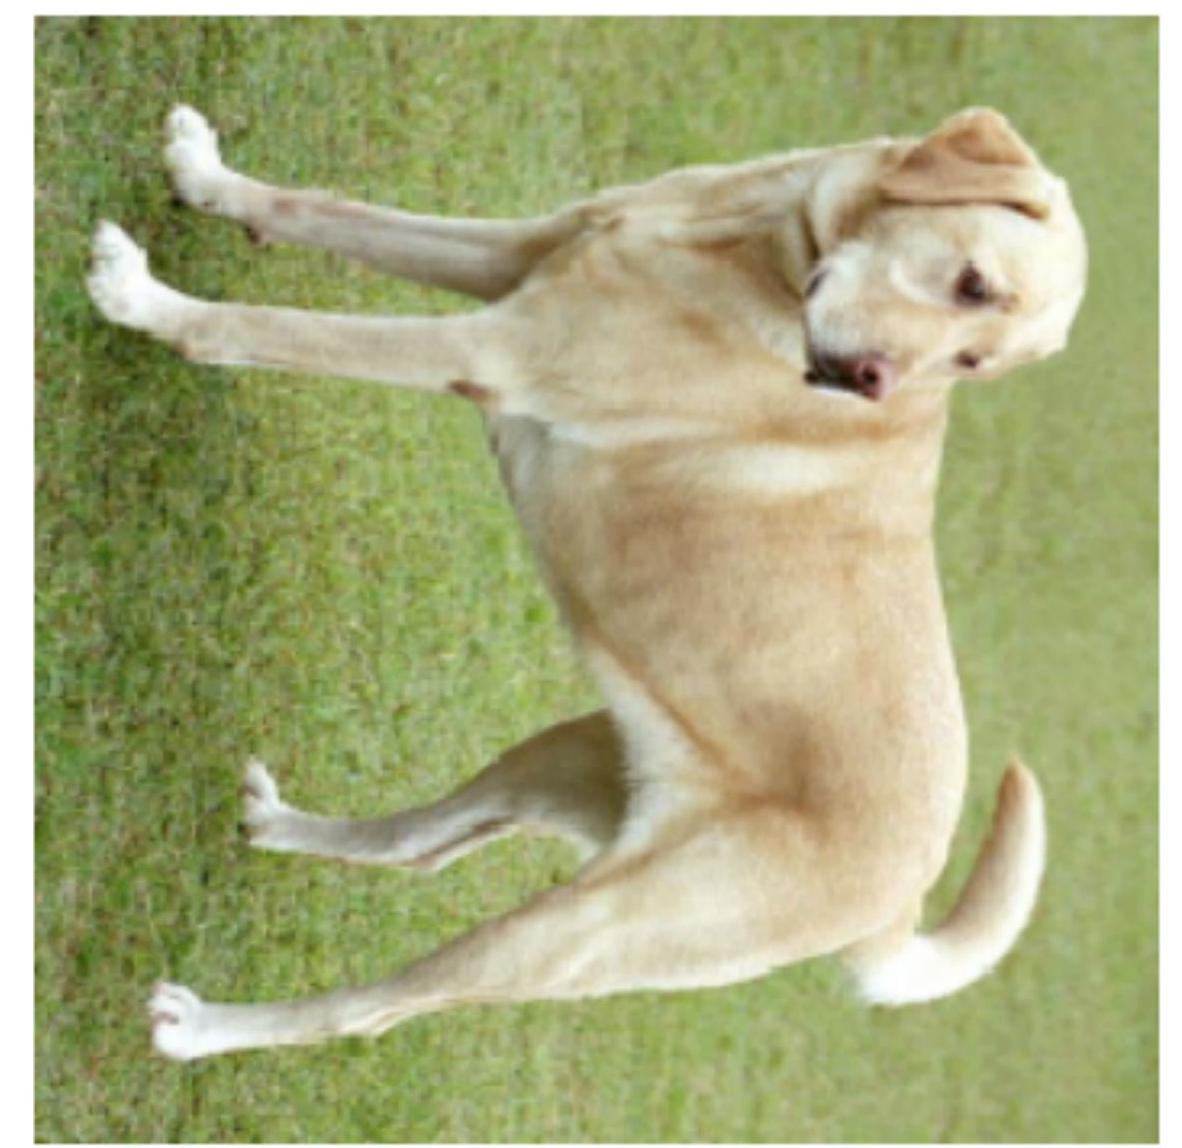
\includegraphics[max width=\textwidth]{2024_01_08_959e2db67a31f073f6d2g-24(1)}
\end{center}

(f) Rotate $\left\{90^{\circ}, 180^{\circ}, 270^{\circ}\right\}$

\begin{center}
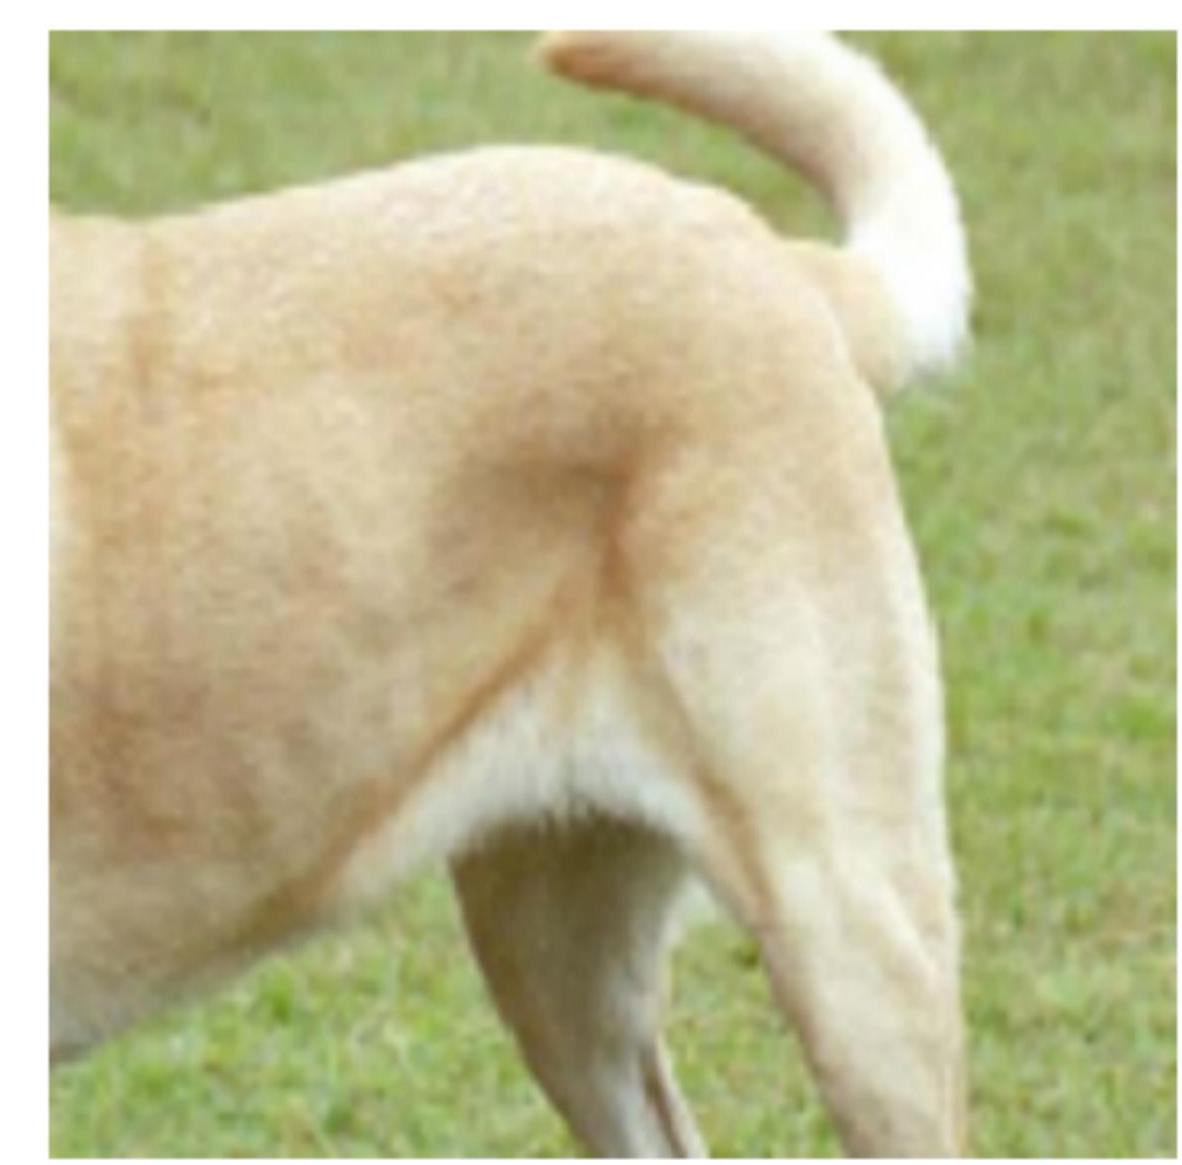
\includegraphics[max width=\textwidth]{2024_01_08_959e2db67a31f073f6d2g-24}
\end{center}

(b) Crop and resize

\begin{center}
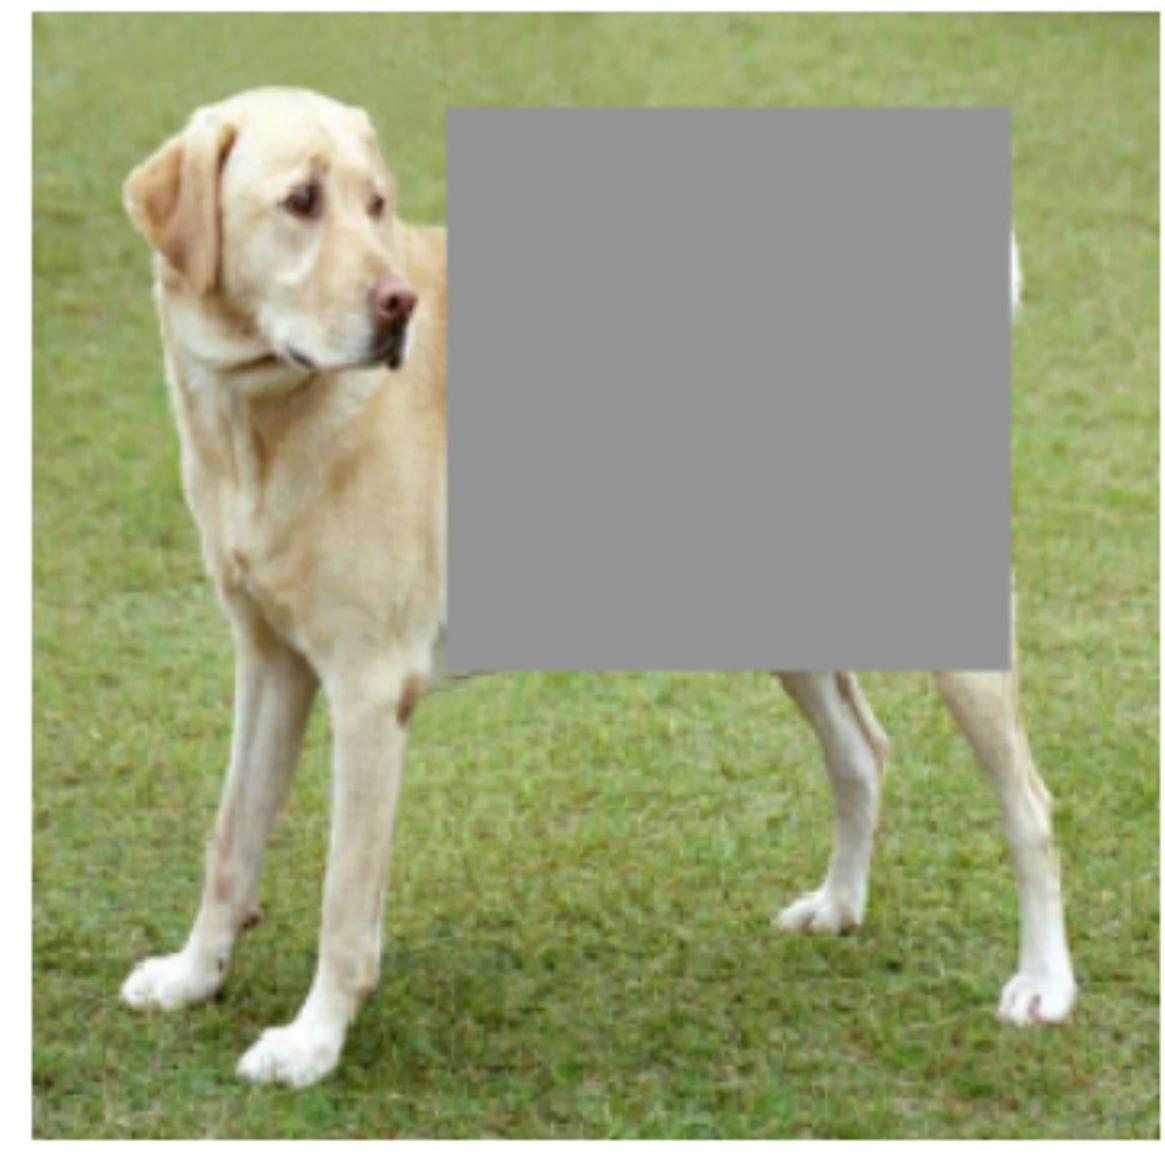
\includegraphics[max width=\textwidth]{2024_01_08_959e2db67a31f073f6d2g-24(4)}
\end{center}

(g) Cutout

\begin{center}
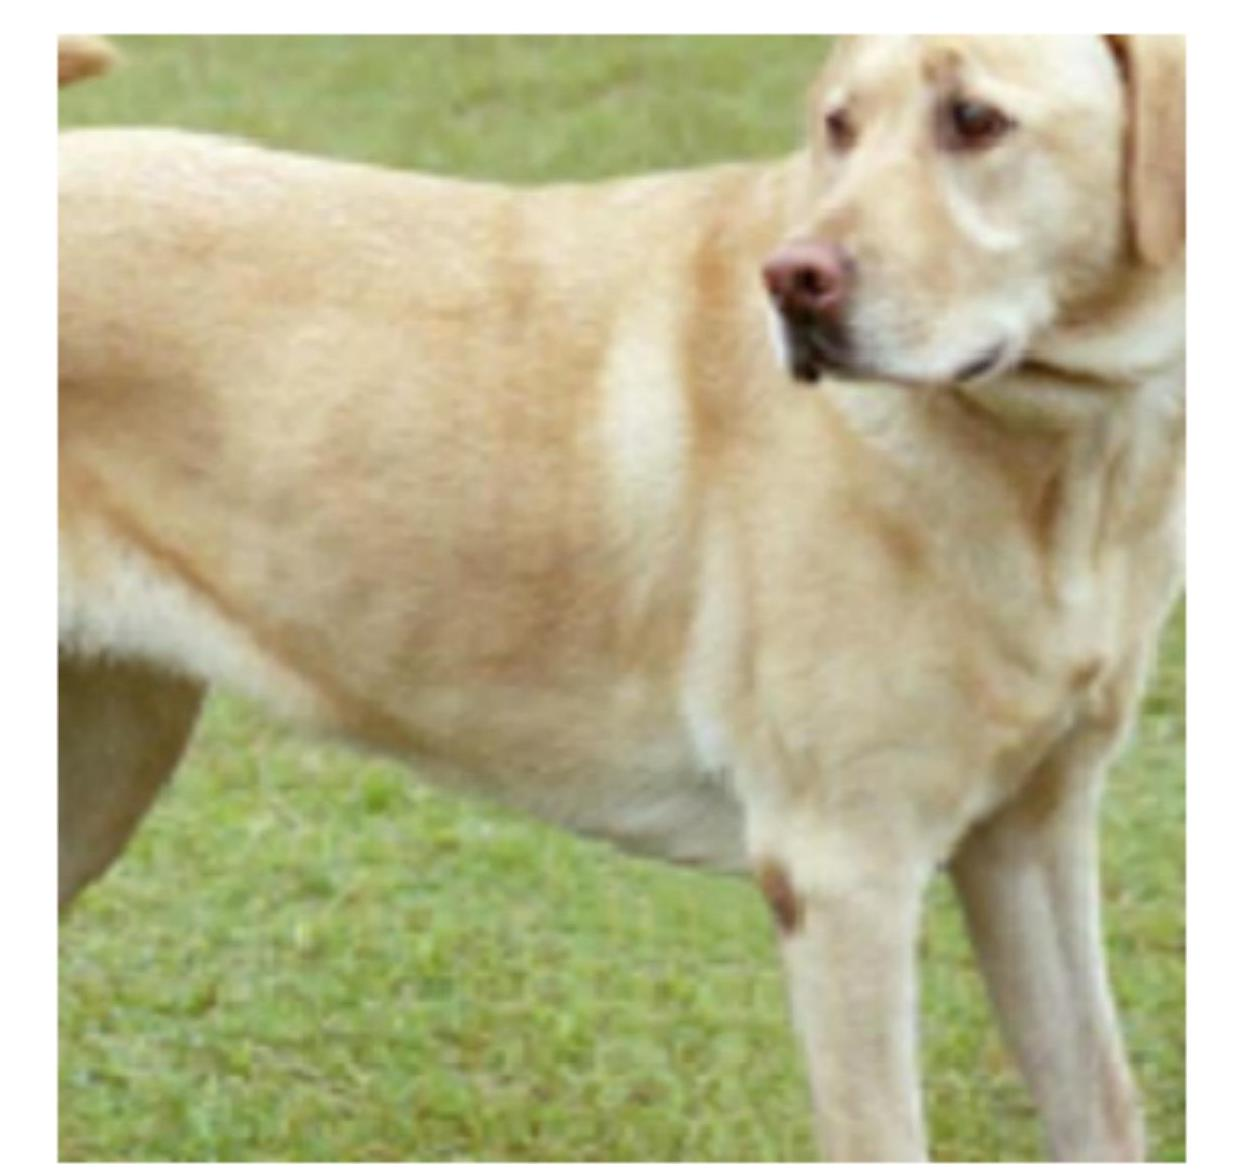
\includegraphics[max width=\textwidth]{2024_01_08_959e2db67a31f073f6d2g-24(2)}
\end{center}

(c) Crop, resize (and flip)

\begin{center}
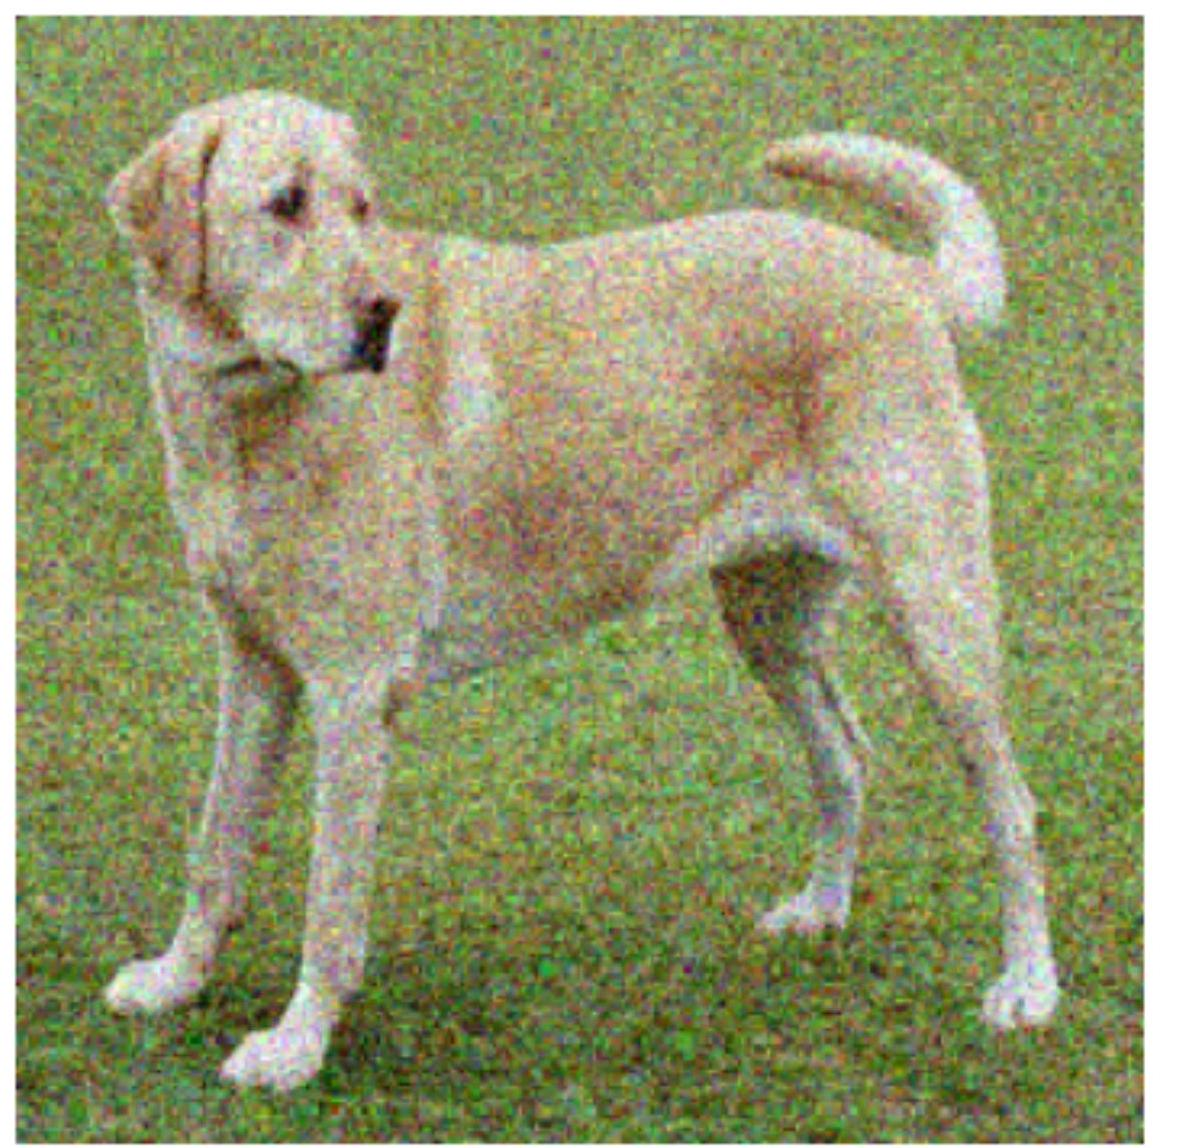
\includegraphics[max width=\textwidth]{2024_01_08_959e2db67a31f073f6d2g-24(8)}
\end{center}

(h) Gaussian noise

\begin{center}
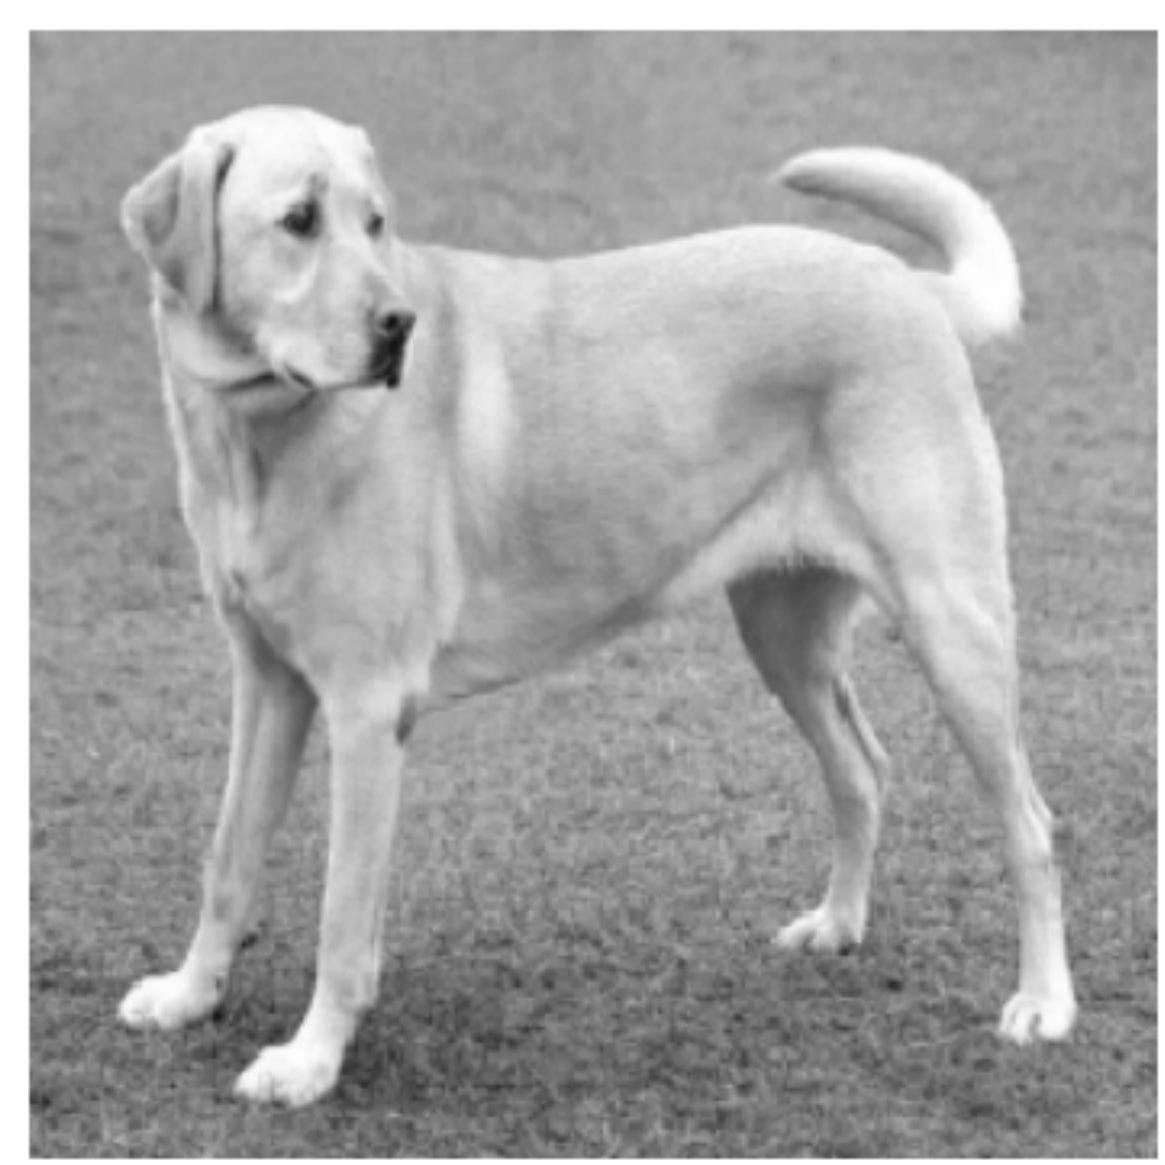
\includegraphics[max width=\textwidth]{2024_01_08_959e2db67a31f073f6d2g-24(6)}
\end{center}

(d) Color distort. (drop)

\begin{center}
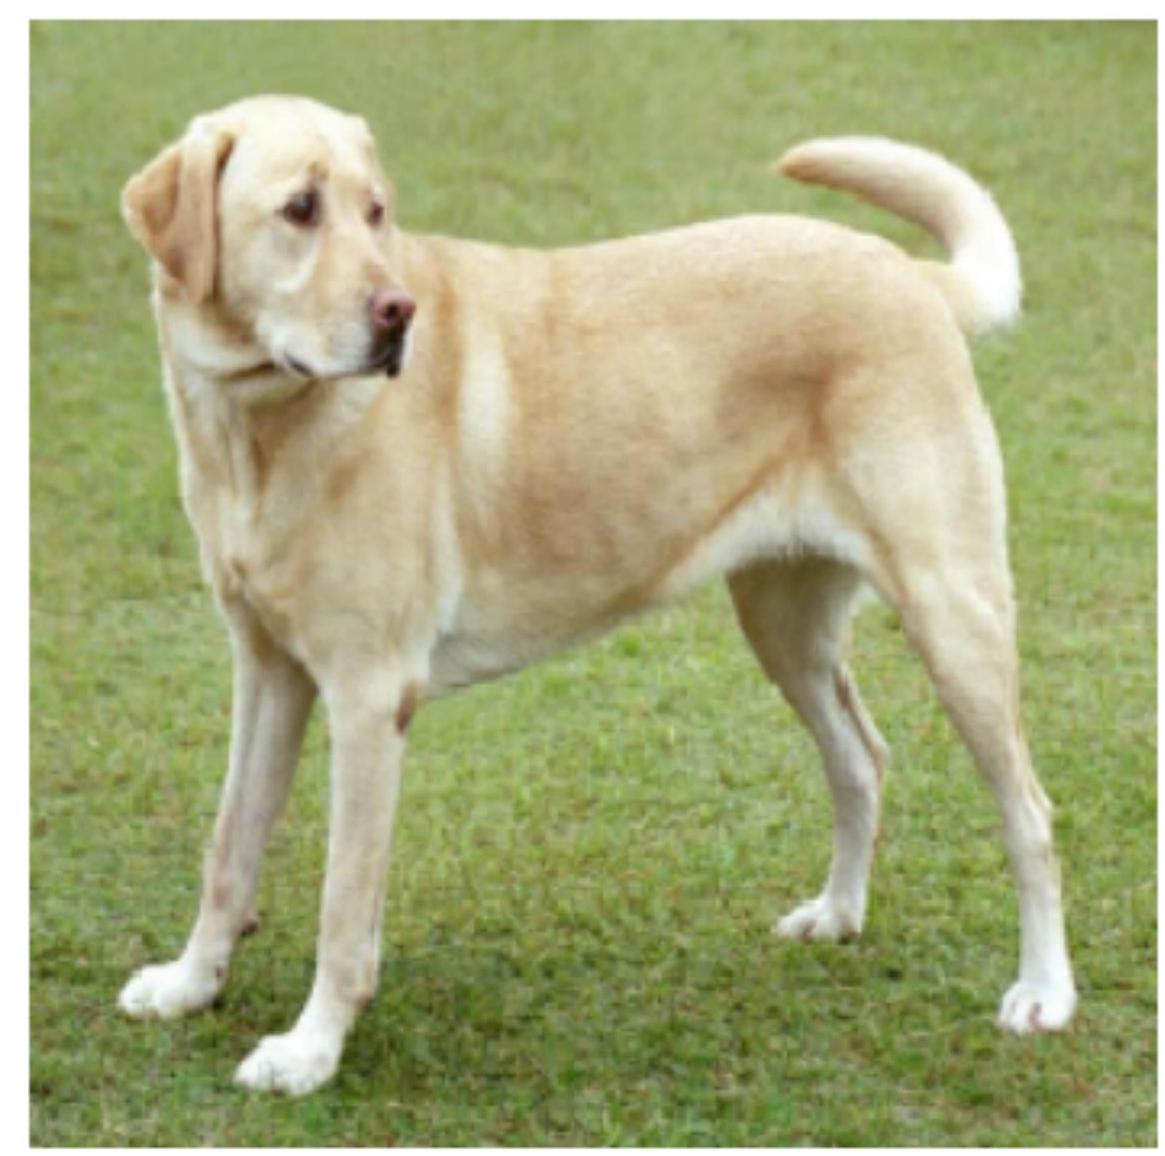
\includegraphics[max width=\textwidth]{2024_01_08_959e2db67a31f073f6d2g-24(5)}
\end{center}

(i) Gaussian blur

\begin{center}
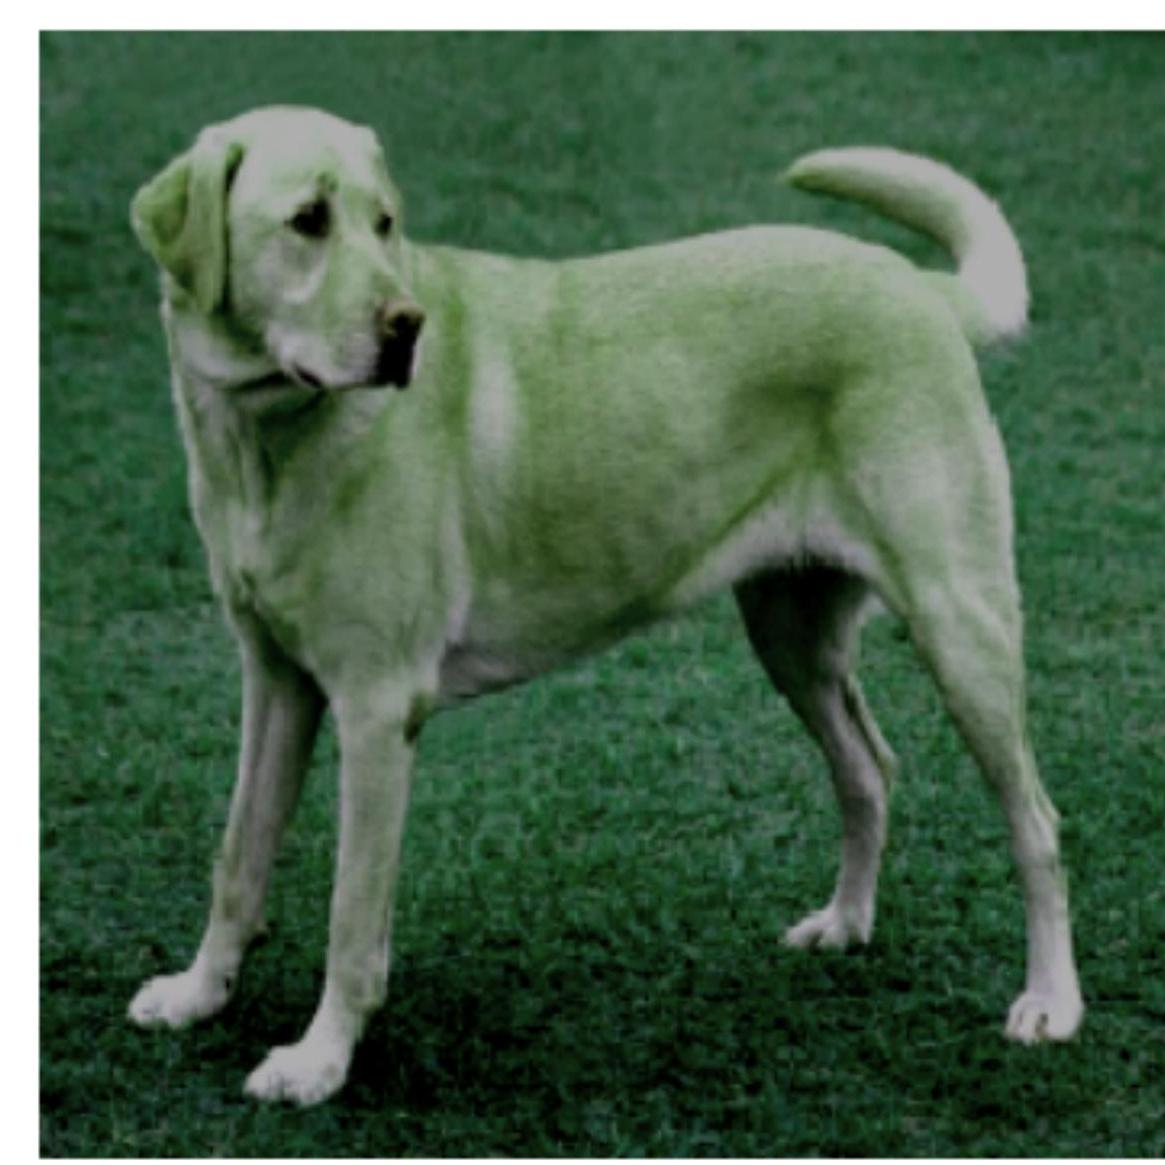
\includegraphics[max width=\textwidth]{2024_01_08_959e2db67a31f073f6d2g-24(7)}
\end{center}

(e) Color distort. (jitter)

\begin{center}
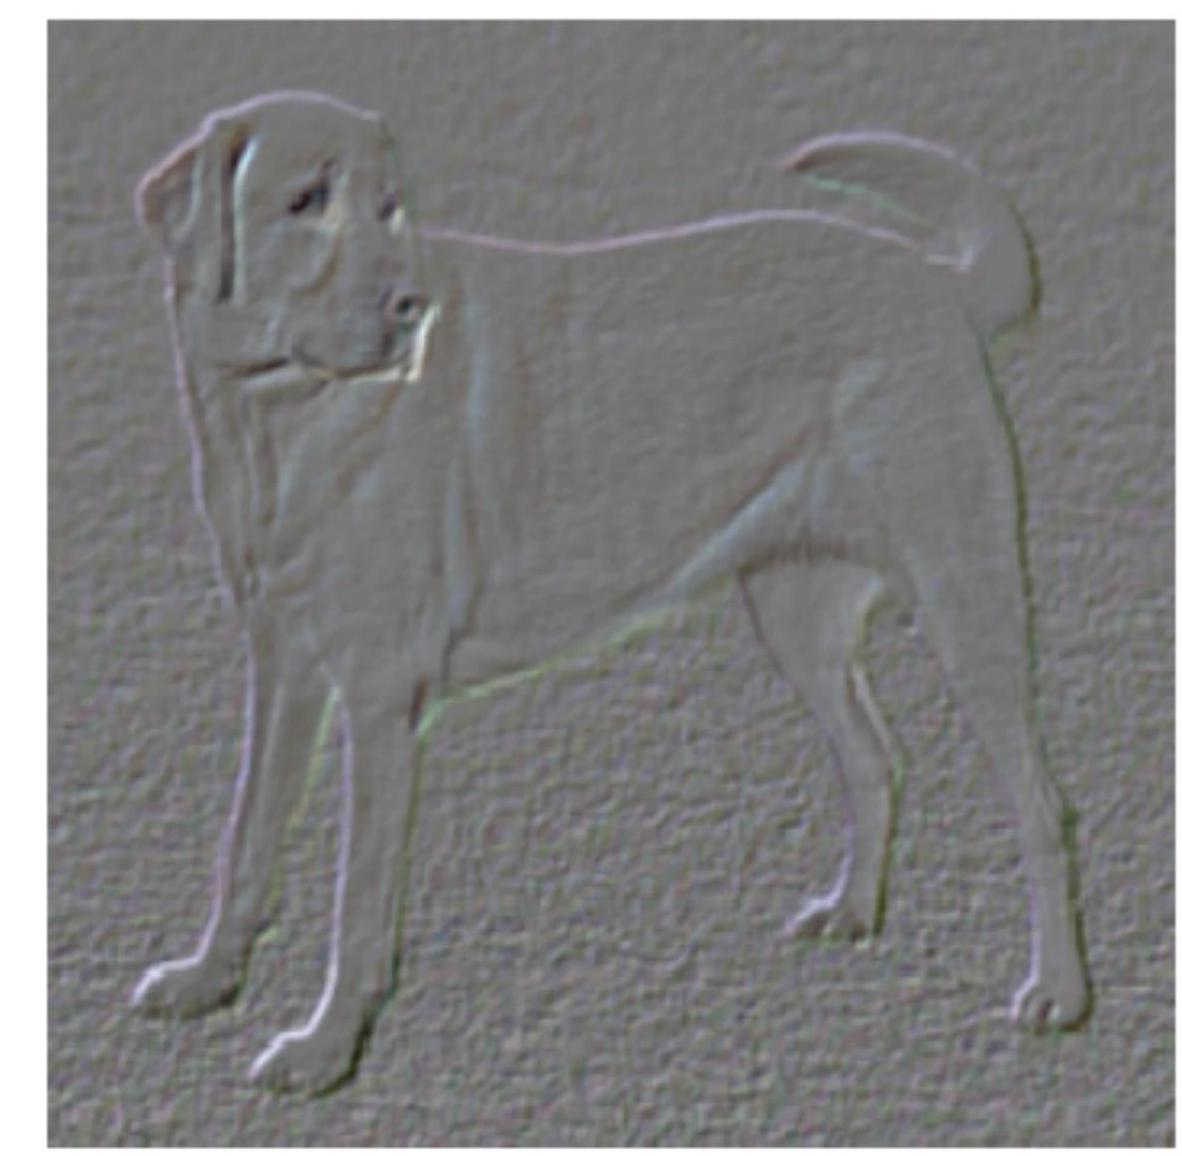
\includegraphics[max width=\textwidth]{2024_01_08_959e2db67a31f073f6d2g-24(9)}
\end{center}

(j) Sobel filtering

T Chen, S Kornblith, M Norouzi, G Hinton. A simple framework for contrastive learning of visual representations. ICML, 2020

\section*{Data augmentation: generated corruptions}
\begin{center}
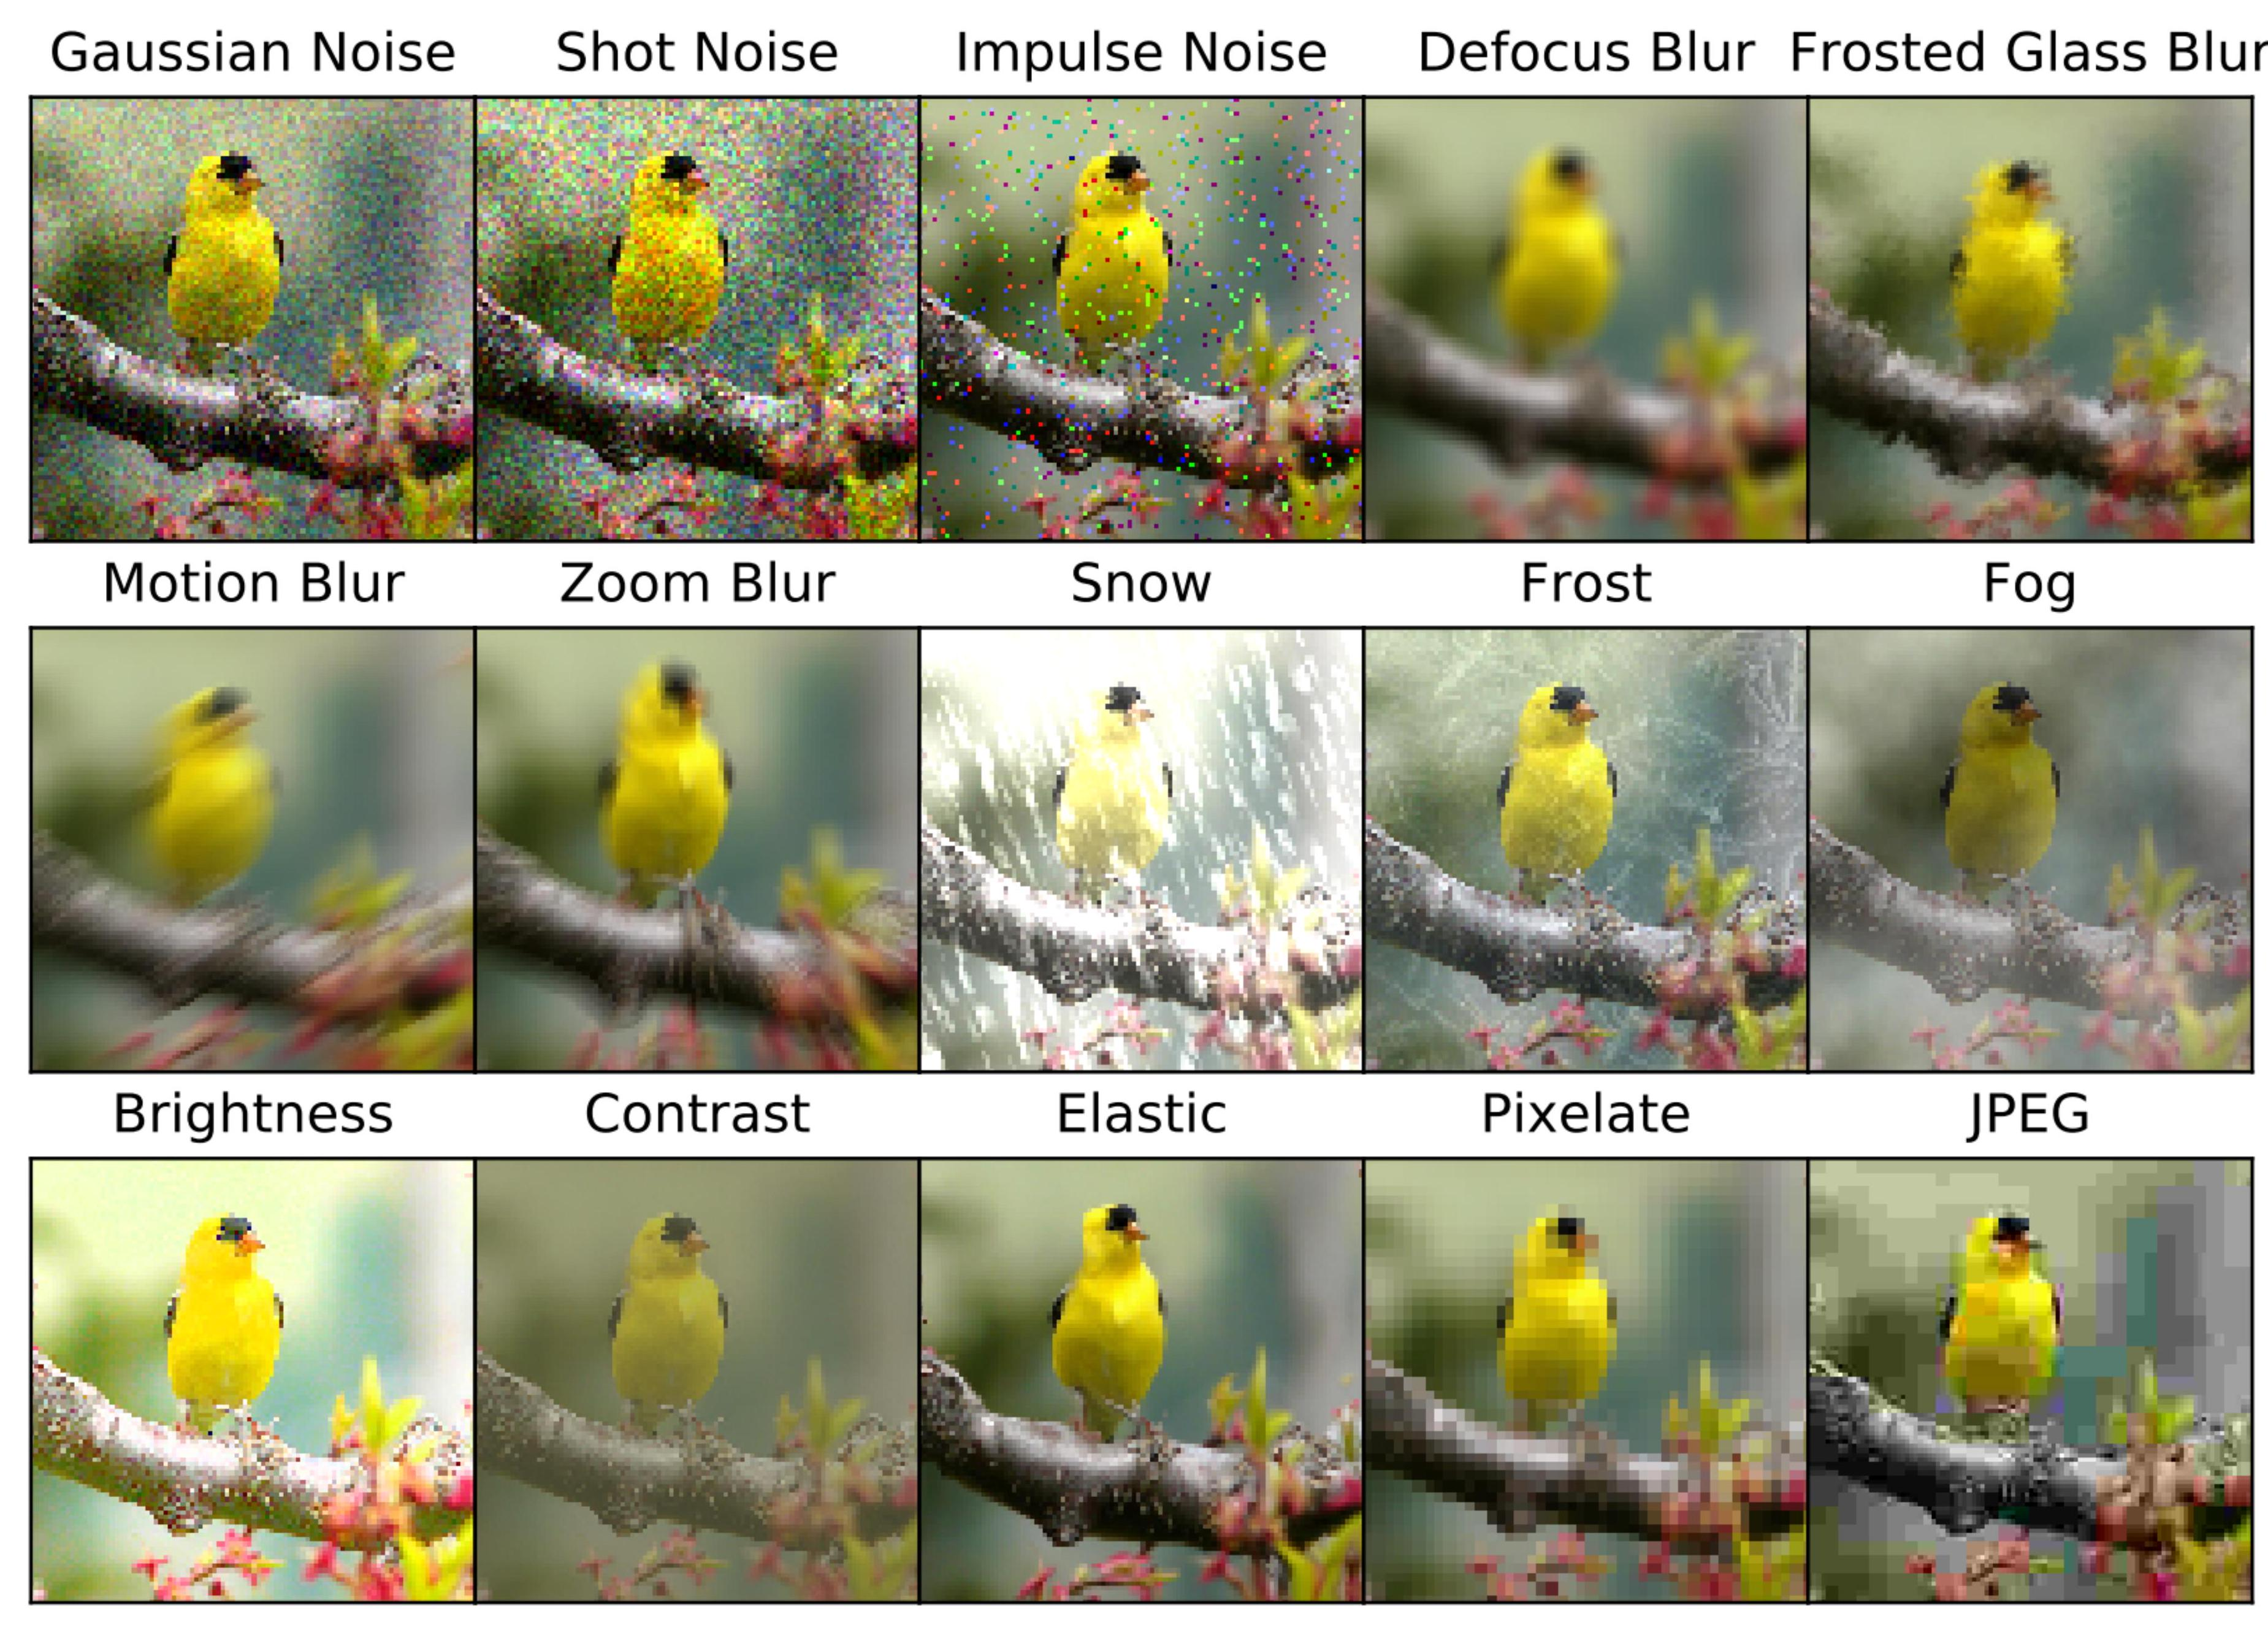
\includegraphics[max width=\textwidth]{2024_01_08_959e2db67a31f073f6d2g-25}
\end{center}

D. Hendrycks and T. Dietterich. Benchmarking Neural Network Robustness to Common Corruptions and Perturbations. ICLR, 2019

Weight Decay

\section*{Weight decay: $l_{2}$-regularization for NNs}
It is standard practice to regularize weights without regularizing bias terms:

$$
\min \mathscr{L}+\frac{\lambda}{2} \sum_{l}\left\|\mathbf{W}^{(l)}\right\|_{F}^{2}
$$

Weight decay [1] favors small weights which can aid in generalization and optimization Optimization with gradient descent:

$$
\left(w_{i, j}^{(l)}\right)_{t+1}=\left(w_{i, j}^{(l)}\right)_{t}-\eta \nabla \mathscr{L}-\eta \lambda\left(w_{i, j}^{(l)}\right)_{t}=\underbrace{(1-\eta \lambda)}_{\text {weight decay }}\left(w_{i, j}^{(l)}\right)_{t}-\eta \nabla \mathscr{L}
$$

Interaction with BatchNorm:

\begin{itemize}
  \item $\mathrm{BN}(\mathbf{W X})=\mathrm{BN}(\alpha \mathbf{W X})$ for $\alpha \in \mathbb{R}_{>0}$ (assuming $\varepsilon \approx 0$ )
  \item $\mathrm{BN}$ is scale invariant in $\mathbf{W}$, hence there is no direct regularization effect from WD
  \item However, the training dynamics differ [2]
\end{itemize}

[1] A. Krogh and J. A Hertz. A simple weight decay can improve generalization. NeurIPS, 1992

[2] R. Wan, et al. Spherical Motion Dynamics: Learning Dynamics of Normalized Neural Network using SGD and Weight Decay. NeurlPS, 2021

Dropout

\section*{Dropout: randomly drop nodes}
Def: At each training step, retain with probability $p^{(l)}$ each node in layer $(l)$ :

\begin{center}
\includegraphics[max width=\textwidth]{2024_01_08_959e2db67a31f073f6d2g-29}
\end{center}

Note: In practice we drop nodes independently for each element of a mini-batch

N. Srivastava, G. Hinton, A. Krizhevsky, I. Sutskever, R. Salakhutdinov. Dropout: A Simple Way to Prevent Neural Networks from Overfitting, JMLR, 2014

\section*{Dropout: training phase}
Def: At each training step, retain with probability $p^{(l)}$ each node in layer $(l)$ :

\begin{center}
\includegraphics[max width=\textwidth]{2024_01_08_959e2db67a31f073f6d2g-30(1)}
\end{center}

Original network

\begin{center}
\includegraphics[max width=\textwidth]{2024_01_08_959e2db67a31f073f6d2g-30}
\end{center}

Random subnetwork

Run one step of SGD on the subnetwork and update the weights

\section*{Dropout: testing phase}
\begin{center}
\includegraphics[max width=\textwidth]{2024_01_08_959e2db67a31f073f6d2g-31}
\end{center}

At training time

When testing:

\begin{itemize}
  \item Use all nodes
\end{itemize}

\begin{center}
\includegraphics[max width=\textwidth]{2024_01_08_959e2db67a31f073f6d2g-31(1)}
\end{center}

At test time

Note: Variance is generally not preserved and as a result Dropout often works

poorly with normalization

\begin{itemize}
  \item Scale each of them by the factor $p^{(l)}$ to ensure that the expected output (when considering the probability of dropping nodes during training) matches the actual output at test time
\end{itemize}

Remark: Weight rescaling can be implemented during training time by scaling the weights by $1 / p^{(l)}$ after each weight update - this is how it is implemented in practice

\section*{Dropout: results}
\begin{itemize}
  \item Setting: Fully-connected networks of different width and depth on MNIST

  \item Dropout results in lower test error

  \item However, dropout typically requires more iterations to converge due to increased stochastic noise

\end{itemize}

\begin{center}
\includegraphics[max width=\textwidth]{2024_01_08_959e2db67a31f073f6d2g-32}
\end{center}

Conclusion

\section*{Entangled effects of various methods: CIFAR10}
\begin{center}
\begin{tabular}{|c|c|c|c|c|c|}
\hline
model & \# parameters & Random crop & Weight decay & Train accuracy & Test accuracy \\
\hline
\multirow{4}{*}{Inception} & \multirow{4}{*}{$1^{\prime} 649^{\prime} 402$} & Yes & Yes & 100.0 & 89.05 \\
\hline
 &  & Yes & No & 100.0 & 89.31 \\
\hline
 &  & No & Yes & 100.0 & 86.03 \\
\hline
 &  & No & No & 100.0 & 85.75 \\
\hline
\multirow{2}{*}{}\begin{tabular}{l}
Inception w/0 \\
BatchNorm \\
\end{tabular} & \multirow{2}{*}{1'649'402} & No & Yes & 100.0 & 83.00 \\
\hline
 &  & No & No & 100.0 & 82.00 \\
\hline
\multirow{4}{*}{Alexnet} & \multirow{4}{*}{1'387'786} & Yes & Yes & 99.90 & 81.22 \\
\hline
 &  & Yes & No & 99.82 & 79.66 \\
\hline
 &  & No & Yes & 100.0 & 77.36 \\
\hline
 &  & No & No & 100.0 & 76.07 \\
\hline
\multirow{2}{*}{MLP $3 \times 512$} & \multirow{2}{*}{1'735'178} & No & Yes & 100.0 & 53.35 \\
\hline
 &  & No & No & 100.0 & 52.39 \\
\hline
\multirow{2}{*}{MLP $1 \times 512$} & \multirow{2}{*}{1'209'866} & No & Yes & 99.80 & 50.39 \\
\hline
 &  & No & No & 100.0 & 50.51 \\
\hline
\end{tabular}
\end{center}

\section*{Entangled effects of various methods: ImageNet}
\begin{center}
\begin{tabular}{|c|c|c|c|c|c|c|c|}
\hline
model & Data aug & Dropout & \begin{tabular}{l}
Weight \\
decay \\
\end{tabular} & \begin{tabular}{l}
Batch \\
Norm \\
\end{tabular} & \begin{tabular}{c}
Skip \\
Connections \\
\end{tabular} & Top-1 train & Top-1 test \\
\hline
\begin{tabular}{l}
ResNet200 \\
(v2) \\
\end{tabular} & Yes & No & Yes & Yes & Yes & ? & 79.9 \\
\hline
\multirow{4}{*}{}\begin{tabular}{l}
Inception \\
(v3) \\
\end{tabular} & Yes & Yes & Yes & Yes & No & 92.18 & 77.84 \\
\hline
 & Yes & No & No & Yes & No & 92.33 & 72.95 \\
\hline
 & No & No & Yes & Yes & No & 90.60 & $67.18(72.57)$ \\
\hline
 & No & No & No & Yes & No & 99.53 & $59.80(63.16)$ \\
\hline
VGG19 & Yes & Yes & Yes & No & No & $?$ & 72.7 \\
\hline
\end{tabular}
\end{center}

() : best test accuracy during training, i.e., with early stopping C Zhang, S Bengio, M Hardt, B Recht, O Vinyals. Understanding deep learning requires rethinking generalization. ICLR, 2017

\section*{Recap}
\begin{itemize}
  \item Convolutional networks are composed of sparsely connected convolutional layers instead of fully-connected linear layers

  \item The same convolution is applied as a sliding window across all spatial locations

  \item Data augmentation usually results in a significant improvement in the model's generalization performance

  \item Weight decay and dropout can further enhance the performance, though typically to a lesser extent

\end{itemize}

\end{document}